%%%%%%%%%%%%%%%%%%%%%%%%%%%%% Thesis.tex %%%%%%%%%%%%%%%%%%%%%%%%%%%%%%%
%                                                                      %
%  ---------- Master of Science Dissertation template ----------       %
%                                                                      %
%  Template for the Master Thesis according to the regulations         %
%  published by the Academic Board (Direcção Académica) at IST.        %
%                                                                      %
%  For up-to-date guide, please refer to the official website          %
%  http://academica.tecnico.ulisboa.pt/alunos/dissertacao-de-mestrado/ %
%                                                                      %
%       Andre C. Marta                                                 %
%       Area Cientifica de Mecanica Aplicada e Aeroespacial            %
%       Departamento de Engenharia Mecanica                            %
%       Instituto Superior Tecnico                                     %
%       Av. Rovisco Pais                                               %
%       1049-001 Lisboa                                                %
%       Portugal                                                       %
%       Tel: +351 21 841 9469                                          %
%                        3469 (extension)                              %
%       Email: andre.marta@tecnico.ulisboa.pt                          %
%                                                                      %
%  Created:       Jan 20, 2011                                         %
%  Last Modified: Feb 19, 2018                                         %
%                                                                      %
%%%%%%%%%%%%%%%%%%%%%%%%%%%%%%%%%%%%%%%%%%%%%%%%%%%%%%%%%%%%%%%%%%%%%%%%
%  Revision history                                                    %
%  v1 - 2011/01/24 - original template                                 %
%  v2 - 2012/10/30 - new IST image and glossary support                %
%  v3 - 2013/12/10 - update according to 2012/13 official guide        %
%  v4 - 2014/02/28 - new default for bibliography style                %
%  v5 - 2014/05/07 - update according to 2013/14 official guide        %
%  v6 - 2015/07/02 - cover page format fixed,                          %
%                    contents page numbering fixed,                    %
%                    better language support,                          %
%                    enhanced examples of tables,                      %
%                    new option for appendix page numbering format,    %
%                    custom bibliography style                         %
%  v7 - 2018/02/19 - multiple citations compressed                     %
%%%%%%%%%%%%%%%%%%%%%%%%%%%%%%%%%%%%%%%%%%%%%%%%%%%%%%%%%%%%%%%%%%%%%%%%
%                                                                      %
% To generate the PDF file, type "make" at the terminal prompt.        %
%                                                                      %
% The IST template LaTeX package was created by the author             %
% and it can be downloaded from:                                       %
% https://fenix.ist.utl.pt/homepage/ist31052/                          %
%                                                                      %
% The external packages can be downloaded from                         %
% the Comprehensive TeX Archive Network at http://www.ctan.org/        %
%                                                                      %
% List of LaTex symbols:                                               %
% http://www.ctan.org/tex-archive/info/symbols/comprehensive/          %
%                                                                      %
% Help with LaTex can be found at                                      %
% http://www.giss.nasa.gov/tools/latex/ltx-2.html                      %
% http://en.wikibooks.org/wiki/LaTeX                                   %
%%%%%%%%%%%%%%%%%%%%%%%%%%%%%%%%%%%%%%%%%%%%%%%%%%%%%%%%%%%%%%%%%%%%%%%%

%%%%%%%%%%%%%%%%%%%%%%%%%%%%%%%%%%%%%%%%%%%%%%%%%%%%%%%%%%%%%%%%%%%%%%%%
%     Preamble                                                         %
%%%%%%%%%%%%%%%%%%%%%%%%%%%%%%%%%%%%%%%%%%%%%%%%%%%%%%%%%%%%%%%%%%%%%%%%

% ----------------------------------------------------------------------
%  Set the document class
% ----------------------------------------------------------------------
\documentclass[10pt,a4paper,twoside]{report}

% ----------------------------------------------------------------------
% Define external packages, language, margins, fonts and new commands
% ----------------------------------------------------------------------
%%%%%%%%%%%%%%%%%%%%%%%%%%%%%%%%%%%%%%%%%%%%%%%%%%%%%%%%%%%%%%%%%%%%%%%%
%                                                                      %
%     File: Thesis_Preamble.tex                                        %
%     Tex Master: Thesis.tex                                           %
%                                                                      %
%     Author: Andre C. Marta                                           %
%     Last modified : 9 Apr 2015                                       %
%                                                                      %
%%%%%%%%%%%%%%%%%%%%%%%%%%%%%%%%%%%%%%%%%%%%%%%%%%%%%%%%%%%%%%%%%%%%%%%%

% ----------------------------------------------------------------------
% Define document language.
% ----------------------------------------------------------------------

% 'inputenc' package
%
% Accept different input encodings.
% http://www.ctan.org/tex-archive/macros/latex/base/
%
% > allows typing non-english text in LaTeX sources.
%
% ******************************* SELECT *******************************
%\usepackage[latin1]{inputenc} % <<<<< Windows
\usepackage[utf8]{inputenc}   % <<<<< Linux
% ******************************* SELECT *******************************


% 'babel' package
%
% Multilingual support for Plain TeX or LaTeX.
% http://www.ctan.org/tex-archive/macros/latex/required/babel/
%
% > sets the variable names according to the language selected
%
% ******************************* SELECT *******************************
%\usepackage[portuguese]{babel} % <<<<< Portuguese
\usepackage[english]{babel} % <<<<< English
% ******************************* SELECT *******************************


% List of LaTeX variable names: \abstractname, \appendixname, \bibname,
%   \chaptername, \contentsname, \listfigurename, \listtablename, ...)
% http://www.tex.ac.uk/cgi-bin/texfaq2html?label=fixnam
%
% Changing the words babel uses (uncomment and redefine as necessary...)
%
\newcommand{\acknowledgments}{@undefined} % new LaTeX variable name
%
% > English
%
\addto\captionsenglish{\renewcommand{\acknowledgments}{Acknowledgments}}
%\addto\captionsenglish{\renewcommand{\contentsname}{Contents}}
%\addto\captionsenglish{\renewcommand{\listtablename}{List of Tables}}
%\addto\captionsenglish{\renewcommand{\listfigurename}{List of Figures}}
%\addto\captionsenglish{\renewcommand{\nomname}{Nomenclature}}
%\addto\captionsenglish{\renewcommand{\glossaryname}{Glossary}}
%\addto\captionsenglish{\renewcommand{\acronymname}{List of Acronyms}}
%\addto\captionsenglish{\renewcommand{\bibname}{References}} % Bibliography
%\addto\captionsenglish{\renewcommand{\appendixname}{Appendix}}

% > Portuguese
%
\addto\captionsportuguese{\renewcommand{\acknowledgments}{Agradecimentos}}
%\addto\captionsportuguese{\renewcommand{\contentsname}{Conte\'{u}do}}
%\addto\captionsportuguese{\renewcommand{\listtablename}{Lista de Figuras}}
%\addto\captionsportuguese{\renewcommand{\listfigurename}{Lista de Tabelas}}
\addto\captionsportuguese{\renewcommand{\nomname}{Lista de S\'{i}mbolos}} % Nomenclatura
%\addto\captionsportuguese{\renewcommand{\glossary}{Gloss\'{a}rio}}
%\addto\captionsportuguese{\renewcommand{\acronymname}{Lista de Abrevia\c{c}\~{o}es}}
%\addto\captionsportuguese{\renewcommand{\bibname}{Refer\^{e}ncias}} % Bibliografia
%\addto\captionsportuguese{\renewcommand{\appendixname}{Anexo}} % Apendice


% ----------------------------------------------------------------------
% Define cover fields in both english and portuguese.
% ----------------------------------------------------------------------
%
\newcommand{\coverThesis}{@undefined} % new LaTeX variable name
\newcommand{\coverSupervisors}{@undefined} % new LaTeX variable name
\newcommand{\coverExaminationCommittee}{@undefined} % new LaTeX variable name
\newcommand{\coverChairperson}{@undefined} % new LaTeX variable name
\newcommand{\coverSupervisor}{@undefined} % new LaTeX variable name
\newcommand{\coverMemberCommittee}{@undefined} % new LaTeX variable name
% > English
\addto\captionsenglish{\renewcommand{\coverThesis}{Thesis to obtain the Master of Science Degree in}}
\addto\captionsenglish{\renewcommand{\coverSupervisors}{Supervisor(s)}}
\addto\captionsenglish{\renewcommand{\coverExaminationCommittee}{Examination Committee}}
\addto\captionsenglish{\renewcommand{\coverChairperson}{Chairperson}}
\addto\captionsenglish{\renewcommand{\coverSupervisor}{Supervisor}}
\addto\captionsenglish{\renewcommand{\coverMemberCommittee}{Member of the Committee}}
% > Portuguese
\addto\captionsportuguese{\renewcommand{\coverThesis}{Disserta\c{c}\~{a}o para obten\c{c}\~{a}o do Grau de Mestre em}}
\addto\captionsportuguese{\renewcommand{\coverSupervisors}{Orientador(es)}}
\addto\captionsportuguese{\renewcommand{\coverExaminationCommittee}{J\'{u}ri}}
\addto\captionsportuguese{\renewcommand{\coverChairperson}{Presidente}}
\addto\captionsportuguese{\renewcommand{\coverSupervisor}{Orientador}}
\addto\captionsportuguese{\renewcommand{\coverMemberCommittee}{Vogal}}


% ----------------------------------------------------------------------
% Define default and cover page fonts.
% ----------------------------------------------------------------------

% Use Arial font as default
%
\renewcommand{\rmdefault}{phv}
\renewcommand{\sfdefault}{phv}

% Define cover page fonts
%
%         encoding     family       series      shape
%  \usefont{T1}     {phv}=helvetica  {b}=bold    {n}=normal
%                   {ptm}=times      {m}=normal  {sl}=slanted
%                                                {it}=italic
% see more examples at
% http://julien.coron.free.fr/languages/latex/fonts/
%
\def\FontLn{% 16 pt normal
  \usefont{T1}{phv}{m}{n}\fontsize{16pt}{16pt}\selectfont}
\def\FontLb{% 16 pt bold
  \usefont{T1}{phv}{b}{n}\fontsize{16pt}{16pt}\selectfont}
\def\FontMn{% 14 pt normal
  \usefont{T1}{phv}{m}{n}\fontsize{14pt}{14pt}\selectfont}
\def\FontMb{% 14 pt bold
  \usefont{T1}{phv}{b}{n}\fontsize{14pt}{14pt}\selectfont}
\def\FontSn{% 12 pt normal
  \usefont{T1}{phv}{m}{n}\fontsize{12pt}{12pt}\selectfont}


% ----------------------------------------------------------------------
% Define page margins and line spacing.
% ----------------------------------------------------------------------

% 'geometry' package
%
% Flexible and complete interface to document dimensions.
% http://www.ctan.org/tex-archive/macros/latex/contrib/geometry/
%
% > set the page margins (2.5cm minimum in every side, as per IST rules)
%
\usepackage{geometry}	
\geometry{verbose,tmargin=2.5cm,bmargin=2.5cm,lmargin=2.5cm,rmargin=2.5cm}

% 'setspace' package
%
% Set space between lines.
% http://www.ctan.org/tex-archive/macros/latex/contrib/setspace/
%
% > allow setting line spacing (line spacing of 1.5, as per IST rules)
%
\usepackage{setspace}
\renewcommand{\baselinestretch}{1.5}


% ----------------------------------------------------------------------
% Include external packages.
% Note that not all of these packages may be available on all system
% installations. If necessary, include the .sty files locally in
% the <jobname>.tex file directory.
% ----------------------------------------------------------------------

% 'graphicx' package
%
% Enhanced support for graphics.
% http://www.ctan.org/tex-archive/macros/latex/required/graphics/
%
% > extends arguments of the \includegraphics command
%
\usepackage{graphicx}


% 'color' package
%
% Colour control for LaTeX documents.
% http://www.ctan.org/tex-archive/macros/latex/required/graphics/
%
% > defines color macros: \color{<color name>}
%
%\usepackage{color}


% 'amsmath' package
%
% Mathematical enhancements for LaTeX.
% http://www.ctan.org/tex-archive/macros/latex/required/amslatex/
%
% > American Mathematical Society plain Tex macros
%
\usepackage{amsmath}  % AMS mathematical facilities for LaTeX.
\usepackage{amsthm}   % Typesetting theorems (AMS style).
\usepackage{amsfonts} % 


% 'wrapfig' package
%
% Produces figures which text can flow around.
% http://www.ctan.org/tex-archive/macros/latex/contrib/wrapfig/
%
% > wrap figures/tables in text (i.e., Di Vinci style)
%
% \usepackage{wrapfig}


% 'subfigure' package
%
% Deprecated: Figures divided into subfigures.
% http://www.ctan.org/tex-archive/obsolete/macros/latex/contrib/subfigure/
%
% > subcaptions for subfigures
%
\usepackage{subfigure}


% 'subfigmat' package
%
% Automates layout when using the subfigure package.
% http://www.ctan.org/tex-archive/macros/latex/contrib/subfigmat/
%
% > matrices of similar subfigures
%
\usepackage{subfigmat}


% 'url' package
%
% Verbatim with URL-sensitive line breaks.
% http://www.ctan.org/tex-archive/macros/latex/contrib/url/
%
% > URLs in BibTex
%
% \usepackage{url}


% 'varioref' package
%
% Intelligent page references.
% http://www.ctan.org/tex-archive/macros/latex/required/tools/
%
% > smart page, figure, table and equation referencing
%
%\usepackage{varioref}


% 'dcolumn' package
%
% Align on the decimal point of numbers in tabular columns.
% http://www.ctan.org/tex-archive/macros/latex/required/tools/
%
% > decimal-aligned tabular math columns
%
\usepackage{dcolumn}
\newcolumntype{d}{D{.}{.}{-1}} % column aligned by the point separator '.'
\newcolumntype{e}{D{E}{E}{-1}} % column aligned by the exponent 'E'


% 'verbatim' package
%
% Reimplementation of and extensions to LaTeX verbatim.
% http://www.ctan.org/tex-archive/macros/latex/required/tools/
%
% > provides the verbatim environment (\begin{verbatim},\end{verbatim})
%   and a comment environment (\begin{comment},  \end{comment})
%
% \usepackage{verbatim}


% 'moreverb' package
%
% Extended verbatim.
% http://www.ctan.org/tex-archive/macros/latex/contrib/moreverb/
%
% > supports tab expansion and line numbering
%
% \usepackage{moreverb}



% 'nomencl' package
%
% Produce lists of symbols as in nomenclature.
% http://www.ctan.org/tex-archive/macros/latex/contrib/nomencl/
%
% The nomencl package makes use of the MakeIndex program
% in order to produce the nomenclature list.
%
% Nomenclature
% 1) On running the file through LATEX, the command \makenomenclature
%    in the preamble instructs it to create/open the nomenclature file
%    <jobname>.nlo corresponding to the LATEX file <jobname>.tex and
%    writes the information from the \nomenclature commands to this file.
% 2) The next step is to invoke MakeIndex in order to produce the
%    <jobname>.nls file. This can be achieved by making use of the
%    command: makeindex <jobname>.nlo -s nomencl.ist -o <jobname>.nls
% 3) The last step is to invoke LATEX on the <jobname>.tex file once
%    more. There, the \printnomenclature in the document will input the
%    <jobname>.nls file and process it according to the given options.
%
% http://www-h.eng.cam.ac.uk/help/tpl/textprocessing/nomencl.pdf
%
% Nomenclature (produces *.nlo *.nls files)
\usepackage{nomencl}
\makenomenclature
%
% Group variables according to their symbol type
%
\RequirePackage{ifthen} 
\ifthenelse{\equal{\languagename}{english}}%
    { % English
    \renewcommand{\nomgroup}[1]{%
      \ifthenelse{\equal{#1}{R}}{%
        \item[\textbf{Roman symbols}]}{%
        \ifthenelse{\equal{#1}{G}}{%
          \item[\textbf{Greek symbols}]}{%
          \ifthenelse{\equal{#1}{S}}{%
            \item[\textbf{Subscripts}]}{%
            \ifthenelse{\equal{#1}{T}}{%
              \item[\textbf{Superscripts}]}{}}}}}%
    }{% Portuguese
    \renewcommand{\nomgroup}[1]{%
      \ifthenelse{\equal{#1}{R}}{%
        \item[\textbf{Simbolos romanos}]}{%
        \ifthenelse{\equal{#1}{G}}{%
          \item[\textbf{Simbolos gregos}]}{%
          \ifthenelse{\equal{#1}{S}}{%
            \item[\textbf{Subscritos}]}{%
            \ifthenelse{\equal{#1}{T}}{%
              \item[\textbf{Sobrescritos}]}{}}}}}%
    }%


% 'glossary' package
%
% Create a glossary.
% http://www.ctan.org/tex-archive/macros/latex/contrib/glossary/
%
% Glossary (produces *.glo *.ist files)
\usepackage[number=none]{glossary}
% (remove blank line between groups)
\setglossary{gloskip={}}
% (redefine glossary style file)
%\renewcommand{\istfilename}{myGlossaryStyle.ist}
\makeglossary


% 'rotating' package
%
% Rotation tools, including rotated full-page floats.
% http://www.ctan.org/tex-archive/macros/latex/contrib/rotating/
%
% > show wide figures and tables in landscape format:
%   use \begin{sidewaystable} and \begin{sidewaysfigure}
%   instead of 'table' and 'figure', respectively.
%
\usepackage{rotating}


% 'hyperref' package
%
% Extensive support for hypertext in LaTeX.
% http://www.ctan.org/tex-archive/macros/latex/contrib/hyperref/
%
% > Extends the functionality of all the LATEX cross-referencing
%   commands (including the table of contents, bibliographies etc) to
%   produce \special commands which a driver can turn into hypertext
%   links; Also provides new commands to allow the user to write adhoc
%   hypertext links, including those to external documents and URLs.
%
\usepackage[pdftex]{hyperref} % enhance documents that are to be
                              % output as HTML and PDF
\hypersetup{colorlinks,       % color text of links and anchors,
                              % eliminates borders around links
%            linkcolor=red,    % color for normal internal links
            linkcolor=black,  % color for normal internal links
            anchorcolor=black,% color for anchor text
%            citecolor=green,  % color for bibliographical citations
            citecolor=black,  % color for bibliographical citations
%            filecolor=magenta,% color for URLs which open local files
            filecolor=black,  % color for URLs which open local files
%            menucolor=red,    % color for Acrobat menu items
            menucolor=black,  % color for Acrobat menu items
%            pagecolor=red,    % color for links to other pages
            pagecolor=black,  % color for links to other pages
%            urlcolor=cyan,    % color for linked URLs
            urlcolor=black,   % color for linked URLs
	          bookmarks=true,         % create PDF bookmarks
	          bookmarksopen=false,    % don't expand bookmarks
	          bookmarksnumbered=true, % number bookmarks
	          pdftitle={Thesis},
            pdfauthor={Andre C. Marta},
            pdfsubject={Thesis Title},
            pdfkeywords={Thesis Keywords},
            pdfstartview=FitV,
            pdfdisplaydoctitle=true}


% 'hypcap' package
%
% Adjusting the anchors of captions.
% http://www.ctan.org/tex-archive/macros/latex/contrib/oberdiek/
%
% > fixes the problem with hyperref, that links to floats points
%   below the caption and not at the beginning of the float.
%
\usepackage[figure,table]{hypcap}


% 'natbib' package
%
% Flexible bibliography support.
% http://www.ctan.org/tex-archive/macros/latex/contrib/natbib/
%
% > produce author-year style citations
%
% \citet  and \citep  for textual and parenthetical citations, respectively
% \citet* and \citep* that print the full author list, and not just the abbreviated one
% \citealt is the same as \citet but without parentheses. Similarly, \citealp is \citep without parentheses
% \citeauthor
% \citeyear
% \citeyearpar
%
%% natbib options can be provided when package is loaded \usepackage[options]{natbib}
%%
%% Following options are valid:
%%
%%   round  -  round parentheses are used (default)
%%   square -  square brackets are used   [option]
%%   curly  -  curly braces are used      {option}
%%   angle  -  angle brackets are used    <option>
%%   semicolon  -  multiple citations separated by semi-colon (default)
%%   colon  - same as semicolon, an earlier confusion
%%   comma  -  separated by comma
%%   authoryear - for author–year citations (default)
%%   numbers-  selects numerical citations
%%   super  -  numerical citations as superscripts, as in Nature
%%   sort   -  sorts multiple citations according to order in ref. list
%%   sort&compress   -  like sort, but also compresses numerical citations
%%   compress - compresses without sorting
%%
% ******************************* SELECT *******************************
%\usepackage{natbib}          % <<<<< References in alphabetical list Correia, Silva, ...
\usepackage[numbers,sort&compress]{natbib} % <<<<< References in numbered list [1],[2],...
% ******************************* SELECT *******************************


% 'notoccite' package
%
% Prevent trouble from citations in table of contents, etc.
% http://ctan.org/pkg/notoccite
%
% > If you have \cite com­mands in \sec­tion-like com­mands, or in \cap­tion,
%   the ci­ta­tion will also ap­pear in the ta­ble of con­tents, or list of what­ever.
%   If you are also us­ing an un­srt-like bib­li­og­ra­phy style, these ci­ta­tions will
%   come at the very start of the bib­li­og­ra­phy, which is con­fus­ing. This pack­age
%   sup­presses the ef­fect.
%
\usepackage{notoccite}


% 'multirow' package
%
% Create tabular cells spanning multiple rows
% http://www.ctan.org/pkg/multirow
%
\usepackage{multirow}


% 'booktabs' package
%
% Publication quality tables in LaTeX
% http://www.ctan.org/pkg/booktabs
%
% > en­hance the qual­ity of ta­bles in LaTeX, pro­vid­ing ex­tra com­mands.
%
% \renewcommand{\arraystretch}{<ratio>} % space between rows
%
\usepackage{booktabs}
%\newcommand{\ra}[1]{\renewcommand{\arraystretch}{#1}}


% 'pdfpages' package
%
% Include PDF documents in LaTeX
% http://www.ctan.org/pkg/pdfpages
%
% > in­clu­sion of ex­ter­nal multi-page PDF doc­u­ments in LaTeX doc­u­ments.
%   Pages may be freely se­lected and sim­i­lar to psnup it is pos­si­ble to put
%   sev­eral log­i­cal pages onto each sheet of pa­per.
%
% \includepdf{filename.pdf}
% \includepdf[pages={4-9},nup=2x3,landscape=true]{filename.pdf}
%
\usepackage{pdfpages}


% ----------------------------------------------------------------------
% Define new commands to assure consistent treatment throughout document
% ----------------------------------------------------------------------

\newcommand{\ud}{\mathrm{d}}                % total derivative
\newcommand{\degree}{\ensuremath{^\circ\,}} % degrees

% Abbreviations

\newcommand{\mcol}{\multicolumn}            % table format

\newcommand{\eqnref}[1]{(\ref{#1})}
\newcommand{\class}[1]{\texttt{#1}}
\newcommand{\package}[1]{\texttt{#1}}
\newcommand{\file}[1]{\texttt{#1}}
\newcommand{\BibTeX}{\textsc{Bib}\TeX}

% Typefaces ( example: {\bf Bold text here} )
%
% > pre-defined
%   \bf % bold face
%   \it % italic
%   \tt % typewriter
%
% > newly defined
\newcommand{\tr}[1]{{\ensuremath{\textrm{#1}}}}   % text roman
\newcommand{\tb}[1]{{\ensuremath{\textbf{#1}}}}   % text bold face
\newcommand{\ti}[1]{{\ensuremath{\textit{#1}}}}   % text italic
\newcommand{\mc}[1]{{\ensuremath{\mathcal{#1}}}}  % math calygraphy
\newcommand{\mco}[1]{{\ensuremath{\mathcalold{#1}}}}% math old calygraphy
\newcommand{\mr}[1]{{\ensuremath{\mathrm{#1}}}}   % math roman
\newcommand{\mb}[1]{{\ensuremath{\mathbf{#1}}}}   % math bold face
\newcommand{\bs}[1]{\ensuremath{\boldsymbol{#1}}} % math symbol
\def\bm#1{\mathchoice                             % math bold
  {\mbox{\boldmath$\displaystyle#1$}}%
  {\mbox{\boldmath$#1$}}%
  {\mbox{\boldmath$\scriptstyle#1$}}%
  {\mbox{\boldmath$\scriptscriptstyle#1$}}}
\newcommand{\boldcal}[1]{{\ensuremath{\boldsymbol{\mathcal{#1}}}}}% math bold calygraphy

 % file "Thesis_Preamble.tex"

%%%%%%%%%%%%%%%%%%%%%%%%%%%%%%%%%%%%%%%%%%%%%%%%%%%%%%%%%%%%%%%%%%%%%%%%
%     Begin Document                                                   %
%%%%%%%%%%%%%%%%%%%%%%%%%%%%%%%%%%%%%%%%%%%%%%%%%%%%%%%%%%%%%%%%%%%%%%%%
\begin{document}

% Set plain page style (no headers, footer with centered page number)
\pagestyle{plain}

% Set roman numbering (i,ii,...) before the start of chapters
\pagenumbering{roman}

% ----------------------------------------------------------------------
%  Cover page
% ----------------------------------------------------------------------
%%%%%%%%%%%%%%%%%%%%%%%%%%%%%%%%%%%%%%%%%%%%%%%%%%%%%%%%%%%%%%%%%%%%%%%%
%                                                                      %
%     File: Thesis_FrontCover.tex                                      %
%     Tex Master: Thesis.tex                                           %
%                                                                      %
%     Author: Andre C. Marta                                           %
%     Last modified :  2 Jul 2015                                      %
%                                                                      %
%%%%%%%%%%%%%%%%%%%%%%%%%%%%%%%%%%%%%%%%%%%%%%%%%%%%%%%%%%%%%%%%%%%%%%%%

\thispagestyle {empty}

% IST Logo - Signature A
% parameters: bb=llx lly urx ury (bounding box), width=h_length, height=v_length, angle=angle, scale=factor, clip=true/false, draft=true/false. 

\includegraphics[bb=9.5cm 11cm 0cm 0cm,scale=0.29]{IST_A_CMYK_POS}

\begin{center}
%
% Figure (Image or plot)
\vspace{7cm}
% height = 50 mm
%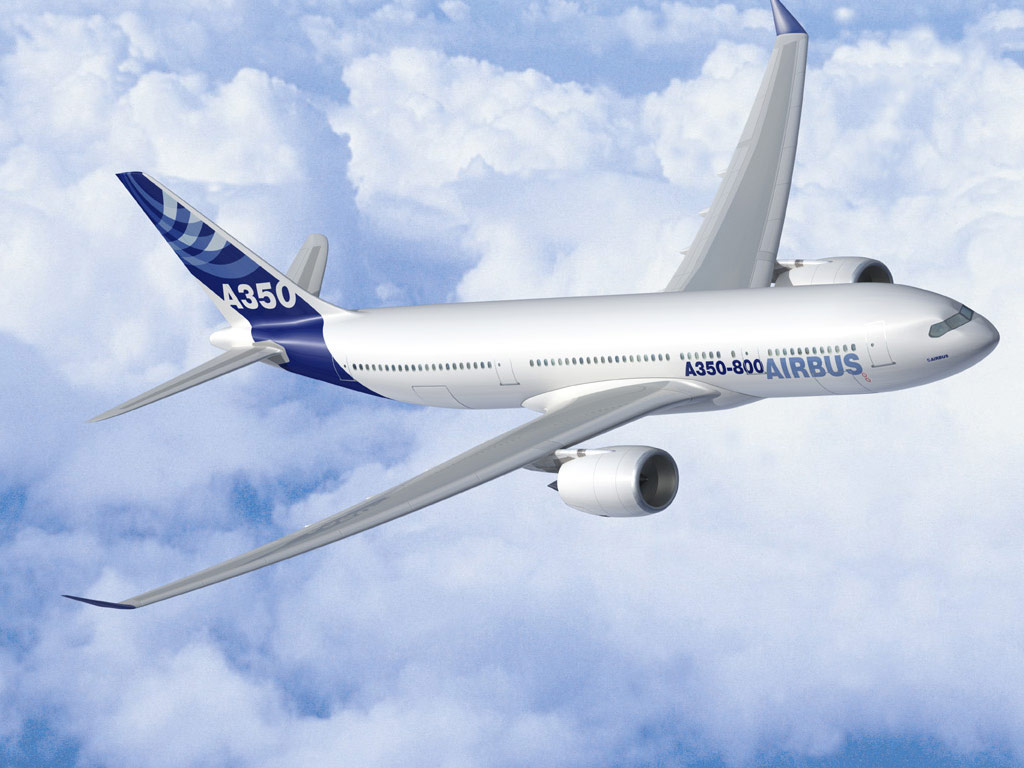
\includegraphics[height=50mm]{Figures/Airbus_A350.jpg}

% Title, author and degree
\vspace{1.0cm}
{\FontLb Thesis Title} \\ % <<<<< EDIT TITLE
%\vspace{0.2cm}
%{\FontMn Subtitle (optional)} \\
%\vspace{1.9cm}
\vspace{2.6cm}
{\FontMb Ana Branca Medeiros Pais} \\ % <<<<< EDIT NAME
\vspace{2.0cm}
{\FontSn \coverThesis} \\
\vspace{0.3cm}
{\FontLb Mathematics and Applications} \\ % <<<<< EDIT COURSE
\vspace{1.0cm}
{\FontSn %
\begin{tabular}{ll}
 \coverSupervisors: &  Professora Doutora Cláudia Rita Ribeiro Coelho Nunes Philippart \\ % <<<<< EDIT NAME
                  %  & Dr. Full Name 2    % <<<<< EDIT NAME
\end{tabular} } \\
\vspace{1.0cm}
{\FontMb \coverExaminationCommittee} \\
\vspace{0.3cm}
{\FontSn %
\begin{tabular}{c}
\coverChairperson:     Professor Doutor António Manuel Pacheco Pires         \\ % <<<<< EDIT NAME
\coverSupervisor:      Professora Doutora Cláudia Rita Ribeiro Coelho Nunes Philippart \\ % <<<<< EDIT NAME
\coverMemberCommittee: Prof. Full Name 3           % <<<<< EDIT NAME
\end{tabular} } \\
\vspace{1.5cm}
{\FontMb October 2018} \\ % <<<<< EDIT DATE (corresponds to date of oral examination)
%
\end{center}

 % file "Thesis_FrontCover.tex"
\cleardoublepage

% ----------------------------------------------------------------------
% Dedication page (optional)
% ----------------------------------------------------------------------
% %%%%%%%%%%%%%%%%%%%%%%%%%%%%%%%%%%%%%%%%%%%%%%%%%%%%%%%%%%%%%%%%%%%%%%%%
%                                                                      %
%     File: Thesis_Dedication.tex                                      %
%     Tex Master: Thesis.tex                                           %
%                                                                      %
%     Author: Andre C. Marta                                           %
%     Last modified :  2 Jul 2015                                      %
%                                                                      %
%%%%%%%%%%%%%%%%%%%%%%%%%%%%%%%%%%%%%%%%%%%%%%%%%%%%%%%%%%%%%%%%%%%%%%%%

\null\vskip5cm%
\begin{flushright}
     Dedicated to someone special...
\end{flushright}
\vfill\newpage

 % file "Thesis_Dedication.tex"
% \cleardoublepage

% ----------------------------------------------------------------------
%  Acknowledgments (optional)
% ----------------------------------------------------------------------
%%%%%%%%%%%%%%%%%%%%%%%%%%%%%%%%%%%%%%%%%%%%%%%%%%%%%%%%%%%%%%%%%%%%%%%%
%                                                                      %
%     File: Thesis_Acknowledgments.tex                                 %
%     Tex Master: Thesis.tex                                           %
%                                                                      %
%     Author: Andre C. Marta                                           %
%     Last modified :  2 Jul 2015                                      %
%                                                                      %
%%%%%%%%%%%%%%%%%%%%%%%%%%%%%%%%%%%%%%%%%%%%%%%%%%%%%%%%%%%%%%%%%%%%%%%%

\section*{\acknowledgments}

% Add entry in the table of contents as section
\addcontentsline{toc}{section}{\acknowledgments}

Apesar deste trabalho estar escrito em inglês não resisto em deixar a nota mais pessoal na minha língua materna.

Começo por agradecer à minha orientadora, a Professora Cláudia,  que muito em cima da hora e a uma distância de quase 2000 km decidiu guiar-me no culminar de cinco anos de estudo. 
Os desafios rapidamente surgiram, assim como as resultantes dúvidas, os progressos na direcção errada e os muito celebrados resultados finais. 
Foi maravilhosa a oportunidade de me ter dado a conhecer as pessoas com quem de perto trabalha e com elas ter partilhado os meus progressos; estupendamente valioso o seu voto de confiança para trabalhar onde me aprouvesse (permitindo-me obter alguns progressos mais relevantes fora de território nacional); e incansável a sua paciência no ping-pong final deste trabalho.

E porque a tese não é fruto apenas dos seis meses em que nela se trabalha, mas antes sim de todo o percurso académico, fora de casa passado, não deixo de agradecer ao pessoal de LMAC que quase família se tornou, pelos muitos cafés, sessões de estudo, churrascos e devaneios; às \textit{soirées do Bob} que sempre serviram para desanuviar das tempestades matemáticas; a todos os amigos que Lausanne me deu e que me ensinaram que as saudades não nos dominam se estivermos em boa companhia e que se consegue realizar (com sucesso!) enormes quantidades de trabalho conjugando muitas horas pelo Rolex e pelo Departamento de Matemática com passeios nos Alpes, idas ao Léman, frutos secos e lutas com colheres de pau no final do dia; e a todos aqueles que surgiram e ficaram (ou se foram), deixando a sua pegada impressa naquilo que hoje sou.

Também, como não poderia deixar de ser, um enorme obrigada a toda a minha família por todo o apoio e conselhos que me dão, por assegurarem que o meu calmo e confortável ninho se encontra sempre de braços abertos para me receber e por todas as infidáveis refeições em que nos reunimos que sempre me deixam de coração cheio. 

Quanto ao futuro, esse é um mistério! Contudo, e por enquanto, toda a minha juventude exclama as palavras de Jack London em "The Call of the Wild",
\begin{flushright}
	\textit{He was mastered by the sheer surging of life,\\
		the tidal wave of being,\\ 
		the perfect joy of each separate muscle, joint,\\
		and sinew in that it was everything that was not death,\\ that it was aglow and rampant,\\
		expressing itself in movement,\\
		flying exultantly under the stars.}
\end{flushright}



 % file "Thesis_Acknowledgements.tex"
\cleardoublepage

% ----------------------------------------------------------------------
%  Abstract (both in English and Portuguese)
% ----------------------------------------------------------------------
%%%%%%%%%%%%%%%%%%%%%%%%%%%%%%%%%%%%%%%%%%%%%%%%%%%%%%%%%%%%%%%%%%%%%%%%
%                                                                      %
%     File: Thesis_Resumo.tex                                          %
%     Tex Master: Thesis.tex                                           %
%                                                                      %
%     Author: Andre C. Marta                                           %
%     Last modified :  2 Jul 2015                                      %
%                                                                      %
%%%%%%%%%%%%%%%%%%%%%%%%%%%%%%%%%%%%%%%%%%%%%%%%%%%%%%%%%%%%%%%%%%%%%%%%

\section*{Resumo}

% Add entry in the table of contents as section
\addcontentsline{toc}{section}{Resumo}

% Add entry in the table of contents as section
\addcontentsline{toc}{section}{Abstract}

Nesta tese a política de investimento óptima relativa a um inovador produto tecnológico é averiguada considerando os seguintes cenários:
\begin{enumerate}
	\item Uma empresa quer investir e entrar no mercado com um novo produto;
	\item Uma empresa já activa quer investir num novo produto, substituindo o antigo; 
	\item Uma empresa já activa quer investir num novo produto, permitindo um período de produção simultânea seguido da substituição total do produto antigo.
\end{enumerate}

Além disso, assumimos que a firma, quando activa, produz um produto estável no mercado e que a decisão de investimento é irreversível, instantanea e pode ser tomada em qualquer altura após o nível the inovação tecnológica desejado ser atingido, pagando os respectivos custos (não reembolsáveis).

Considerando que a procura evolui de acordo com um Movimento Geométrico Browniano e que o nível de inovação segue um Processo de Poisson Composto, derivamos o nível de procura que justifica o investmento para cada uma das situações referidas, seguido da sua análise comparativa. Estudamos ainda a sensibilidade do tempo até o investimento óptimo e o impacto do investimento em pesquisa e desenvolvimento (P\&D) no processo de investimento, através de análises quer analíticas quer numéricas.

Posto isto, esta tese pretende ser uma ajuda na actual indústria tecnológica, pelo forneceminto de ferramentas poderosas para as equipas de decisão, assim como pelas suas contribuições para literatura em Matemática Financeira, em particular na área de Investimento sob Incerteza.






\vfill

\textbf{\Large Palavras-Chave:} Problemas de Paragem Óptima; Abordagem de Opções Reais; Investimento Sob Incerteza; Inovação Tecnológica.
   % file "Thesis_Resumo.tex"
\cleardoublepage

%%%%%%%%%%%%%%%%%%%%%%%%%%%%%%%%%%%%%%%%%%%%%%%%%%%%%%%%%%%%%%%%%%%%%%%%
%                                                                      %
%     File: Thesis_Abstract.tex                                        %
%     Tex Master: Thesis.tex                                           %
%                                                                      %
%     Author: Andre C. Marta                                           %
%     Last modified :  2 Jul 2015                                      %
%                                                                      %
%%%%%%%%%%%%%%%%%%%%%%%%%%%%%%%%%%%%%%%%%%%%%%%%%%%%%%%%%%%%%%%%%%%%%%%%

\section*{Abstract}

% Add entry in the table of contents as section
\addcontentsline{toc}{section}{Abstract}

In this thesis the optimal investment policy regarding an innovative technological product is addressed under the following scenarios:
\begin{enumerate}
	\item A firm wants to invest and enter the market with a new product;
	\item An active firm wants to invest and launch a new product, that totally replaces the old one; 
	\item An active firm wants to invest and launch a new product, allowing a temporarily simultaneous production period, followed by the old product's total replacement.
\end{enumerate}

Moreover, we assume that the firm, when active, produces an established product and that the investment decision is irreversible, instantaneous, has an associate (sunk) cost and can be made at any time after a desired innovation level is reached.

Considering the demand to evolve as a Geometric Brownian Motion and innovation level accordingly to a Compound Poisson Process, we derive the demand level(s) that justifies the investment decision(s) in each situation along with the respective comparative statics analysis. Lastly, the sensitivity of optimal investment times and the impact of R\&D investment in the innovation process are also analysed either analytically or numerically. 

Overall, this thesis expects to complement modern IT industry, providing powerful tools for decision support teams, and to bring relevant contributions to the literature on Financial Mathematics, particularly to the Investment under Uncertainty field.





\vfill

\textbf{\Large Keywords:} Optimal Stopping Problems; Real Options Approach; Investment Under Uncertainty; Technology Innovation.

 % file "Thesis_Abstract.tex"
\cleardoublepage

% ----------------------------------------------------------------------
%  Table of contents, list of tables, list of figures and nomenclature
% ----------------------------------------------------------------------

% Table of contents
%
\tableofcontents
\cleardoublepage 

% List of tables
%
% Add entry in the table of contents as section
\phantomsection
\addcontentsline{toc}{section}{\listtablename}
% Generate list
\listoftables
\cleardoublepage 

% List of figures
%
% Add entry in the table of contents as section
\phantomsection
\addcontentsline{toc}{section}{\listfigurename}
% Generate list
\listoffigures
\cleardoublepage 

% Nomenclature
%
% entries of nomenclature list
%%%%%%%%%%%%%%%%%%%%%%%%%%%%%%%%%%%%%%%%%%%%%%%%%%%%%%%%%%%%%%%%%%%%%%%%
%                                                                      %
%     File: Thesis_Nomenclature.tex                                    %
%     Tex Master: Thesis.tex                                           %
%                                                                      %
%     Author: Andre C. Marta                                           %
%     Last modified : 21 Jan 2011                                      %
%                                                                      %
%%%%%%%%%%%%%%%%%%%%%%%%%%%%%%%%%%%%%%%%%%%%%%%%%%%%%%%%%%%%%%%%%%%%%%%%
%
% The definitions can be placed anywhere in the document body
% and their order is sorted by <symbol> automatically when
% calling makeindex in the makefile
%
% The \glossary command has the following syntax:
%
% \glossary{entry}
%
% The \nomenclature command has the following syntax:
%
% \nomenclature[<prefix>]{<symbol>}{<description>}
%
% where <prefix> is used for fine tuning the sort order,
% <symbol> is the symbol to be described, and <description> is
% the actual description.

% ----------------------------------------------------------------------
% Roman symbols [r]
\nomenclature[ru]{$\bf u$}{Velocity vector.}
\nomenclature[ru]{$u,v,w$}{Velocity Cartesian components.}
\nomenclature[rp]{$p$}{Pressure.}
\nomenclature[rC]{$C_D$}{Coefficient of drag.}
\nomenclature[rC]{$C_L$}{Coefficient of lift.}
\nomenclature[rC]{$C_M$}{Coefficient of moment.}

% ----------------------------------------------------------------------
% Greek symbols [g]
\nomenclature[g]{$\rho$}{Density.}
\nomenclature[g]{$\alpha$}{Angle of attack.}
\nomenclature[g]{$\beta$}{Angle of side-slip.}
\nomenclature[g]{$\mu$}{Molecular viscosity coefficient.}
\nomenclature[g]{$\kappa$}{Thermal conductivity coefficient.}

% ----------------------------------------------------------------------
% Subscripts [s]
\nomenclature[s]{$x,y,z$}{Cartesian components.}
\nomenclature[s]{$i,j,k$}{Computational indexes.}
\nomenclature[s]{$\infty$}{Free-stream condition.}
\nomenclature[s]{ref}{Reference condition.}
\nomenclature[s]{$n$}{Normal component.}

% ----------------------------------------------------------------------
% Supercripts [t]
\nomenclature[t]{T}{Transpose.}
\nomenclature[t]{*}{Adjoint.}

 % file "Thesis_Nomenclature.tex"
\cleardoublepage 
%
% Add entry in the table of contents as section
\phantomsection
\addcontentsline{toc}{section}{\nomname}
% Insert glossary/nomenclature section produced by MakeIndex
\printnomenclature
\cleardoublepage

% entries of glossary list
%%%%%%%%%%%%%%%%%%%%%%%%%%%%%%%%%%%%%%%%%%%%%%%%%%%%%%%%%%%%%%%%%%%%%%%%
%                                                                      %
%     File: Thesis_Glossary.tex                                        %
%     Tex Master: Thesis.tex                                           %
%                                                                      %
%     Author: Andre C. Marta                                           %
%     Last modified : 30 Oct 2012                                      %
%                                                                      %
%%%%%%%%%%%%%%%%%%%%%%%%%%%%%%%%%%%%%%%%%%%%%%%%%%%%%%%%%%%%%%%%%%%%%%%%
%
% The definitions can be placed anywhere in the document body
% and their order is sorted by <symbol> automatically when
% calling makeindex in the makefile
%
% The \glossary command has the following syntax:
%
% \glossary{entry}
%
% The \nomenclature command has the following syntax:
%
% \nomenclature[<prefix>]{<symbol>}{<description>}
%
% where <prefix> is used for fine tuning the sort order,
% <symbol> is the symbol to be described, and <description> is
% the actual description.

% ----------------------------------------------------------------------

\glossary{name={\textbf{MDO}},description={Multi-Disciplinar Optimization is an engineering technique that uses optimization methods to solve design problems incorporating two or more disciplines.}}

\glossary{name={\textbf{CFD}},description={Computational Fluid Dynamics is a branch of fluid mechanics that uses numerical methods and algorithms to solve problems that involve fluid flows.}}

\glossary{name={\textbf{CSM}},description={Computational Structural Mechanics is a branch of structure mechanics that uses numerical methods and algorithms to perform the analysis of structures and its components.}}

 % file "Thesis_Glossary.tex"

% Add entry in the table of contents as section
\phantomsection
\addcontentsline{toc}{section}{\glossaryname}
% Insert glossary section produced by MakeIndex
\printglossary
\cleardoublepage

% Set arabic numbering (1,2,...) after preface
%
\setcounter{page}{1}
\pagenumbering{arabic}

% ----------------------------------------------------------------------
%  Chapters
% ----------------------------------------------------------------------

%%%%%%%%%%%%%%%%%%%%%%%%%%%%%%%%%%%%%%%%%%%%%%%%%%%%%%%%%%%%%%%%%%%%%%%%
%                                                                      %
%     File: Thesis_Introduction.tex                                    %
%     Tex Master: Thesis.tex                                           %
%                                                                      %
%     Author: Andre C. Marta                                           %
%     Last modified :  2 Jul 2015                                      %
%                                                                      %
%%%%%%%%%%%%%%%%%%%%%%%%%%%%%%%%%%%%%%%%%%%%%%%%%%%%%%%%%%%%%%%%%%%%%%%%

\chapter{Introduction}
\label{chapter:introduction}


%%%%%%%%%%%%%%%%%%%%%%%%%%%%%%%%%%%%%%%%%%%%%%%%%%%%%%%%%%%%%%%%%%%%%%%%
\section{Motivation}
\label{section:motivation}

Nowadays, society is highly attached to technology, from mobile phones to fancy gadgets - and sometimes scratching the absurd
\footnote{Parents forget to feed child while playing videogames:\\
\url{https://www.theguardian.com/world/2010/mar/05/korean-girl-starved-online-game} }.
 Nevertheless, all this huge demand brought changes on how IT companies should manage their investments. These should, not only pay attention to the product demand on the market, but also to technology evolution. Therefore investors began to require more complex models to support their decisions. Models must not only consider the current value of the firm, such as the ones based on the Net Present Value (NPV), but also must take into account the potential associated to future events.

We may consider as an example ASML, a dutch company considered to be the largest european semiconductor equipment maker which currently is part of Euro Stoxx 50\footnote{Stock index representing the 50 most liquid stocks in the Eurozone:\\  \url{http://en.boerse-frankfurt.de/index/constituents/Euro_Stoxx_50\#Constituents} }.
ASML builds electronic chips producing machines that satisfy the needs of hardware building companies - for instance, Intel and Samsung\footnote{For further details check: \url{https://www.asml.com/company/our-history/en/s277?rid=51985}}.
Therefore, in order to survive on the competitive market, ASML needs either to develop their own technology, by investing on R\&D, or to import a desired one, with an associated cost.

This work is focused on the case where the firm chooses to develop their own technology and, hence, define \textit{a priori} the desired innovation level and investment to be made. Since it is impossible to access that a certain level of technology will be reached in a precise amount of time\footnote{Flying cars predicted for 2015 in \textit{Back to Future} as an example (!):\\  \url{http://content.time.com/time/specials/packages/article/0,28804,2024839_2024845_2024855,00.html}} \footnote{Moore's Law - which defends that processor performance doubles (approximately) every two years - is dying:\\
\url{https://www.forbes.com/sites/forbestechcouncil/2018/03/09/moores-law-is-dying-so-where-are-its-heirs/\#53cb24a17a7b}}, the innovation process is considered to evolve randomly with time, with a rate that might be influenced by the amount of money invested. More money implies more resources and, hence, an higher evolution rate.

After %having reached 
reaching the desired innovation level, the firm must evaluate under which market conditions it should invest and in which type of products. The final goal is to maximize the expected long run profit.


%iPhone X release in 2017:\\ \url{https://www.bloomberg.com/news/articles/2017-11-02/long-lines-are-back-at-apple-stores-for-10th-anniversary-iphone
%}}



%%%%%%%%%%%%%%%%%%%%%%%%%%%%%%%%%%%%%%%%%%%%%%%%%%%%%%%%%%%%%%%%%%%%%%%%

\section{State-of-the-art}

%Quite many recent works
%suggest that Real Option\footnote{Real Option's concept will be defined on Section \ref{bc_ro}.} analysis is much more advantageous than the Net Present Value (NPV) analysis when it comes to support investment decisions, since the last one assumes that the company has a now or never approach regarding the investment decision, ignoring the freedom in timing.
%and hence it ignores the option of having a better situation in the future. 
%On the other side a Real Option Analysis takes into account the future potential, as well the respective uncertainty.
%Among many studies already made, Farzin \textit{et al.} (1998) \cite{farzin:cap}, do a comparative study between both approaches in the technology adoption context.

One of the first contributions on Real Options analysis regarding investment decisions was due to McDonald \& Siegel (1986)  \cite{siegel}. They model an investment problem where the investor must decide when it is the best time to exercise the option, taking into account that the value of the investment project is stochastically random and evolves accordingly to a Geometric Brownian Motion. Other contributions were due to Dixit (1989) \cite{dixit_alone}, who models the best time to make entry and exit decisions, while considering that the market price evolves accordingly to a Brownian Motion and that each decision has an associated cost.

The study by Dixit \& Pindyck (1994) \cite{dixit:book}, that is nowadays considered the financial by some Bible of Real Options approach, exploits an analogy between real options and financial investment decisions, focusing on many different decision problems (entry, investment and exit, among them) dependent on different stochastically behavioured (diffusion processes and jump diffusion processes, among them) measures, such as demand or market price.

%Some other topics regarding Real Option increased their relevance. More particularly, the optimal production capacity to be chosen and the impact of technology adoption - being this last one a field of increasing interest nowadays.

As our understanding about the market of new technological products evolved, the optimal production capacity to be chosen and the impact of technology adoption associated to investment decisions have started to get more relevant.

%Regarding optimal production capacity, 
In the aspect of optimal capacity production Huisman \& Kort (2013) \cite{huis:cap} proposed a methodology to estimate the best time and capacity to invest in a new product. Both monopoly and a duopoly situations were assumed on their study.

Regarding technology adoption,
Farzin \textit{et al.} (1998) \cite{farzin:cap}, presented a comparative study between NPV and Real Option approaches in the context that a firm wants to deduce when is the best time and level to invest in a technology.
Also, Hagspiel \textit{et al.} (2016) \cite{hagspiel:cap} studied the best time to invest in a new product or exit the market, by considering a firm whose established product has a declining profit and a demand process to evolve accordingly to a GBM. %The solution leads to three different demand thresholds for the respective possible decisions.


Recently, Pimentel (2018) \cite{rita} explored both optimal capacity level and technology adoption. By considering two sources of uncertainty, related to the demand and the innovation processes,
%- the demand to evolve as a jump diffusion process and the innovation process as a compound Poisson process - 
and a firm which is producing an established product, she deduces the optimal times to invest in a new product and to stop the production of the established product. 
%Regarding the described situation, two models were developed: the benchmark model and the capacity optimization model.



%In this work we will also consider the demand to be stochastically, evolving accordingly to a Geometric Brownian Motion. On the third optimal stopping problem, on Section \ref{chapter:3}, we will also derive three different thresholds, although these are related with the possibility of either invest in a new product with simultaneous production of the new and the established product and then stop the production of the established product or invest on the new product and immediately replace the established product. A similar situation was already presented by Pimentel \cite{rita}, however in a different context. On her work, she considers two sources of uncertain - which strongly influence each of the thresholds derived -, while in our work we only consider one, the demand level already referred. 




%%%%%%%%%%%%%%%%%%%%%%%%%%%%%%%%%%%%%%%%%%%%%%%%%%%%%%%%%%%%%%%%%%%%%%%%
\section{Thesis Outline}
\label{section:outline}


This thesis is organized in eight chapters.

The first one consists in the present introduction, which includes the state-of-the-art and the main context of the problem considered along this thesis.

%Considering the context described on Section \ref{section:context}, we will treat three different situations related with the irreversible decision of investing in a new product when the innovation breakthrough and future demand are stochastic.

%\textcolor{red}{1 SOURCE OF UNCERATINTY (DEMAND) OU 2 (INNOVATION PROCESS)?}

The major theoretical concepts are introduced on Chapter \ref{chapter:bc}, following several approaches presented in the literature (references \cite{dixit:book}, \cite{ross} and \cite{oksendal:book}).
We start by exploring the most relevant results of Optimal Stopping Problems (OSP). Then we show how they are related to investment decisions under uncertainty through Real Option analysis.

On the next three chapters we analyse different possible investment decisions, namely:
\begin{itemize}
	\item Chapter \ref{chapter:1}: a firm that has no products in the market and wants to find the optimal time to introduce a new product;
	\item Chapter \ref{chapter:2}: a firm with an established product in the market wants to find the optimal time to invest in a new product while replacing immediately the old one;
	\item Chapter \ref{chapter:3}: a firm with an established product wants to find the optimal time to invest in a new product.
	Two scenarios are considered:
	 \begin{enumerate}
	 	\item The old product is immediately replaced;
	 	\item A simultaneous production period is allowed and followed by the removal of the oldest product.
	 \end{enumerate}
	% while either replacing immediately the established product by the new one or allowing a simultaneous production period, followed by the removal of the oldest product.
\end{itemize}

%conditions

Two models are developed for situations described on Chapters \ref{chapter:1} and \ref{chapter:2}. The first one corresponds to the benchmark model, which considers the original cash-flow for a chosen production capacity. The second one to the capacity optimization model, which considers the maximized long-run cash-flow with respect to production capacity. 
Regarding the situation described on Chapter \ref{chapter:3}, due to its complexity, only the benchmark model is analysed.
On the last section of each of the three chapters we study the behaviour of respective thresholds and optimal capacity level with different parameters.


The behaviour of optimal investment times, associated to the situations described on chapters 3 to 5, regarding initial demand values and market's uncertainty is studied on Chapter \ref{chapter:stoptime}.



On Chapter \ref{chapter:max} we derive the optimal R\&D investment, by maximizing the expected value function with respect to the innovation process. 
First, we derive the optimal R\&D investment considering that the innovation process only takes one jump to achieve the breakthrough level.
Secondly, we generalize the previous situation by considering that the innovation process takes $n \in \mathds{N}$ jumps to achieve the breakthrough level.
In the end of this chapter, the behaviour of the decision threshold with the different parameters is studied.



Finally, on Chapter \ref{chapter:conc} we summarize the relevant findings and how this work can be extended.


%%%%%%%%%%%%%%%%%%%%%%%%%%%%%%%%%%%%%%%%%%%%%%%%%%%%%%%%%%%%%%%%%%%%%%%%
\section{Problem Context}
\label{section:context}

In the current work we consider a firm that develops its own technology and decides to invest in a new product only after an innovation breakthrough, associated to innovation level $\theta$.


The innovation process associated to the technology level is denoted by $\{ \theta(t), \ t \geq 0 \}$ and considered to be an homogeneous Compound Poisson process, evolving accordingly to
$$\theta_t= \theta_0+ u N_t$$  
where $\theta_0$ corresponds to the initial innovation level, $u > 0$ to the jump size in the technology and $\{N_t, \ t \geq 0\}$  to the jump process, which follows a Poisson process with rate $\lambda(R)=R^\gamma, \ \gamma \in (0,1)$, where $R$ stands for the R\&D investment, such as scientist salaries, equipment costs and expenses. The mentioned rate function $\lambda$ is such that it verifies:
\begin{itemize}
	\item $\lambda(0) = 0$: no R\&D investment means zero probability of innovating;
	\item $\lambda^\prime (R)>0$: the larger the investment is, the higher is the probability of observing a jump. Hence, the waiting time for the next technology jump is expect to be shorter;
	\item $ \lambda ^{ \prime \prime} (R)<0$: exists an optimal R\&D investment that leads to the maximization of the rate function, that is, $\exists R^*: \lambda(R^*)\geq \lambda(R), \  \forall R$.
\end{itemize}

%Under this situation the firms decides how much it will invest in R\&D, knowing that a bigger investment implies a smaller expected time until it is able to invest on the new product.

When the breakthrough happens, the innovation process stops and the firm is able to decide when it should invest on the new product with the innovation level $\theta$. In order to have the new product available on the market, the firm needs to incur an investment (sunk) cost. This one is related with employees' formation and new equipment, for example, that depends on the production capacity chosen $K_1$. In this work, it is assumed that the firm produces up to its full capacity. Hence sunk costs will be dependent on the quantity of production chosen.

Since the new product offers a new technology level, not recognized by the market, its profit is strongly dependent on market's demand. The better the reception of the product, the bigger the demand and the corresponding profit.
%Here the demand is considered to evolve accordingly to a Geometric Brownian Motion (GBM) which initial state corresponds to the demand at the breakthrough time.

%The investment decision will be influenced by the long run profit possible to be obtained.

The goal of this work is to define,
%using realoptions analysis,
the optimal investment time on a new product. The estimation of this time takes into account Real Options analysis, how market conditions influences it and 
%hat 
the maximization of the expected long run profit.
% is maximized and to study how market conditions influence it.

In the following sections we will consider the timeline represented in the schematic diagram below in Figure \ref{0_time}.

%%%%%%%%%%%%%%%%%%%%%%%%%%%%%%%%%%%%%%%%%%%%%%%%%%%%%%%%%
%
%
%\begin{tikzpicture}[y=1cm, x=1cm, thick, font=\footnotesize]    
%\usetikzlibrary{arrows,decorations.pathreplacing}
%
%\tikzset{
%	brace_top/.style={
%		decoration={brace},
%		decorate
%	},
%	brace_bottom/.style={
%		decoration={brace, mirror},
%		decorate
%	}
%}
%
%% time line week
%\draw[line width=1.2pt, ->, >=latex'](0,0) -- coordinate (x axis) (14,0) node[right] {\textit{Time}}; 
%\foreach \x in {0,3,8}
%\draw (\x cm,3pt) -- (\x cm,-3pt);
%%\foreach \x in {current time,  , $\tau$, 3} \draw (\x,0.1) -- (\x,-0.1) node[below] {\x};
%\draw (0,0) node[below=3pt] (a) {$\text{R\&D investment}$} node[above=3pt] {};
%\draw (3,0) node[below=9pt] (a) {$\text{Innovation breakthrough $\theta$\\
%	$t_1=0$}$} node[above=3pt] {};
%\draw (8,0) node[below=3pt] (a) {$\tau:$ 
%\text{ \textit{new} product's investment\\ $t_2=0$: initial instant regarding $\tau_2$}} node[above=3pt] {};
%\draw (12,0) node[below=9pt] (a) {$\tau_2:$ \text{\textit{old} product's abandonment}} node[above=3pt] {};
%
%%brace
%%\node (start_p) at (0,0.6) {};
%%\node (end_p) at (7.99,0.6) {};
%%\draw [brace_top] (start_p.north) -- node [above, pos=0.5] {$\text{\textit{Old} product}$} (end_p.north);
%
%%brace
%%\node (start_pn) at (8.01,0.6) {};
%%\node (end_pn) at (11.99,0.6) {};
%%\draw [brace_top] (start_pn.north) -- node [above, pos=0.5] {$\text{\textit{Old \& New} product}$} (end_pn.north);
%
%%brace
%\node (start_pn) at (8.01,0.6) {};
%\node (end_pn) at (13.8,0.6) {};
%\draw [brace_top] (start_pn.north) -- node [above, pos=0.5] {$\text{\textit{New} product}$} (end_pn.north);
%
%
%% top brace
%\node (start_t) at (0,0.1) {};
%\node (end_t) at (2.99,0.1) {};
%\draw [brace_top] (start_t.north) -- node [above, pos=0.5] {$\text{Innovation development}$} (end_t.north);
%
%% top brace
%\node (start_week) at (3.01,0.1) {};
%\node (end_week) at (13.8,0.1) {};
%\draw [brace_top] (start_week.north) -- node [above, pos=0.5] {$\text{Firm is able to make its investment decisions regarding $\theta$}$} (end_week.north);
%
%\end{tikzpicture}


%%%%%%%%%%%%%%%%%%%%%%%%%%%%%%%%%%%%%%%%%%%%%%%%%%%%%%%%%%%

%\vspace{4mm}
%%\begin{figure}[h]
%%	\centering
%	\begin{tikzpicture}[y=1cm, x=1cm, thick, font=\footnotesize]    
%	\usetikzlibrary{arrows,decorations.pathreplacing}
%	
%	\tikzset{
%		brace_top/.style={
%			decoration={brace},
%			decorate
%		},
%		brace_bottom/.style={
%			decoration={brace, mirror},
%			decorate
%		}
%	}
%	
%	% time line week
%	\draw[line width=1.2pt, ->, >=latex'](0,0) -- coordinate (x axis) (14,0) node[right] {\textit{Time}}; 
%	\foreach \x in {0,3}
%	\draw (\x cm,3pt) -- (\x cm,-3pt);
%	%\foreach \x in {current time,  , $\tau$, 3} \draw (\x,0.1) -- (\x,-0.1) node[below] {\x};
%	\draw (0,0) node[below=3pt] (a) {$\text{R\&D investment}$} node[above=3pt] {};
%	\draw (3,0) node[below=9pt] (a) {$\text{Innovation breakthrough $\theta$}$} node[above=3pt] {};
%	
%	%%brace
%	%\node (start_p) at (0,0.6) {};
%	%\node (end_p) at (7.99,0.6) {};
%	%\draw [brace_top] (start_p.north) -- node [above, pos=0.5] {$\text{\textit{Old} product}$} (end_p.north);
%	%
%	%%brace
%	%\node (start_pn) at (8.01,0.6) {};
%	%\node (end_pn) at (11.99,0.6) {};
%	%\draw [brace_top] (start_pn.north) -- node [above, pos=0.5] {$\text{\textit{Old \& New} product}$} (end_pn.north);
%	%
%	%%brace
%	%\node (start_pn) at (12.01,0.6) {};
%	%\node (end_pn) at (13.8,0.6) {};
%	%\draw [brace_top] (start_pn.north) -- node [above, pos=0.5] {$\text{\textit{New} product}$} (end_pn.north);
%	
%	
%	% top brace
%	\node (start_t) at (0,0.1) {};
%	\node (end_t) at (2.99,0.1) {};
%	\draw [brace_top] (start_t.north) -- node [above, pos=0.5] {$\text{Innovation development}$} (end_t.north);
%	
%	% top brace
%	\node (start_week) at (3.01,0.1) {};
%	\node (end_week) at (13.8,0.1) {};
%	\draw [brace_top] (start_week.north) -- node [above, pos=0.5] {$\text{Firm is able to make its investment decisions regarding $\theta$}$} (end_week.north);
%	
%	\end{tikzpicture}
%
%
%
%
%
%	
%%%brace
%%\node (start_p) at (0,0.6) {};
%%\node (end_p) at (7.99,0.6) {};
%%\draw [brace_top] (start_p.north) -- node [above, pos=0.5] {$\text{\textit{Old} product}$} (end_p.north);
%%
%%%brace
%%\node (start_pn) at (8.01,0.6) {};
%%\node (end_pn) at (11.99,0.6) {};
%%\draw [brace_top] (start_pn.north) -- node [above, pos=0.5] {$\text{\textit{Old \& New} product}$} (end_pn.north);
%%
%%%brace
%%\node (start_pn) at (12.01,0.6) {};
%%\node (end_pn) at (13.8,0.6) {};
%%\draw [brace_top] (start_pn.north) -- node [above, pos=0.5] {$\text{\textit{New} product}$} (end_pn.north);

%%%%%%%%%%%%%%%%%%%%%%%%%%%%%%%%%%%%%%%%%%%%%%%%%%%%%%%%%


\begin{figure}[h]
	\centering
	\vspace{4mm}
	%\begin{figure}[h]
	%	\centering
	\begin{tikzpicture}[y=1cm, x=1cm, thick, font=\footnotesize]    
	\usetikzlibrary{arrows,decorations.pathreplacing}
	
	
	
	% time line week
	\draw[line width=1.2pt, ->, >=latex'](0,0) -- coordinate (x axis) (14,0) node[right] {\textit{Time}}; 
	\foreach \x in {0,3}
	\draw (\x cm,3pt) -- (\x cm,-3pt);
	%\foreach \x in {current time,  , $\tau$, 3} \draw (\x,0.1) -- (\x,-0.1) node[below] {\x};
	\draw (0,0) node[below=3pt] (a) {$\text{R\&D investment}$} node[above=3pt] {};
	\draw (3,0) node[below=9pt] (a) {$\text{Innovation breakthrough $\theta$}$} node[above=3pt] {};
	
	%%brace
	%\node (start_p) at (0,0.6) {};
	%\node (end_p) at (7.99,0.6) {};
	%\draw [brace_top] (start_p.north) -- node [above, pos=0.5] {$\text{\textit{Old} product}$} (end_p.north);
	%
	%%brace
	%\node (start_pn) at (8.01,0.6) {};
	%\node (end_pn) at (11.99,0.6) {};
	%\draw [brace_top] (start_pn.north) -- node [above, pos=0.5] {$\text{\textit{Old \& New} product}$} (end_pn.north);
	%
	%%brace
	%\node (start_pn) at (12.01,0.6) {};
	%\node (end_pn) at (13.8,0.6) {};
	%\draw [brace_top] (start_pn.north) -- node [above, pos=0.5] {$\text{\textit{New} product}$} (end_pn.north);
	
	
	% top brace
	\node (start_t) at (0,0.1) {};
	\node (end_t) at (2.99,0.1) {};
	\draw [brace_top] (start_t.north) -- node [above, pos=0.5] {$\text{Innovation development}$} (end_t.north);
	
	% top brace
	\node (start_week) at (3.01,0.1) {};
	\node (end_week) at (13.8,0.1) {};
	\draw [brace_top] (start_week.north) -- node [above, pos=0.5] {$\text{Firm is able to make its investment decisions regarding $\theta$}$} (end_week.north);
	
	\end{tikzpicture}
	
	\caption{Timeline representing the innovation development and the investment period. Time is set to start at the innovation breakthrough.}
	\label{0_time}
\end{figure}






Henceforth, when determining the optimal investment time on the new product, we consider as the starting time the instant at which occurs the innovation breakthrough. However when evaluating the value function regarding the complete investment (associated to both R\&D and new product), the starting time corresponds to the time at which the firm decides to invest in R\&D.






 % file "Thesis_Introduction.tex"
\cleardoublepage

%%%%%%%%%%%%%%%%%%%%%%%%%%%%%%%%%%%%%%%%%%%%%%%%%%%%%%%%%%%%%%%%%%%%%%%%
%                                                                      %
%     File: Thesis_Implementation.tex                                  %
%     Tex Master: Thesis.tex                                           %
%                                                                      %
%     Author: Andre C. Marta                                           %
%     Last modified :  2 Jul 2015                                      %
%                                                                      %
%%%%%%%%%%%%%%%%%%%%%%%%%%%%%%%%%%%%%%%%%%%%%%%%%%%%%%%%%%%%%%%%%%%%%%%%

\chapter{Background concepts}
\label{chapter:bc1}

Before starting to explain the work that is here developed, we introduce the main concepts and tools required.

We will start by introducing the field of Optimal Control Problems: defining its key elements, deducing the dynamic programming principle, respective dynamic programming equation and the verification technique. Secondly, we will explain how they are related with the field of optimal stopping problems as well as how we can find an optimal stopping time. Lastly, we will explain how Optimal Stopping Problems are related with investment decisions under uncertainty, deducing the general solution of the (standard) optimal problems that we will face along this work.

%%%%%%%%%%%%%%%%%%%%%%%%%%%%%%%%%%%%%%%%%%%%%%%%%%%%%%%%%%%%%%%%%%%%%%%%

\section{Stochastic Control and Optimal Stopping Problems}
\label{section:scop}	

\subsection{Stochastic Control Problems}
\label{section:control}

\subsubsection{Settings}

We need to set the key elements related to stochastic control problems. Among these, it is included:

\textbf{Time Horizon:}
in the context of investment-consumption problems (as this work is), an infinite time-horizon is considered: $[0,\infty)$. However one may also consider a finite horizon: $[0,T], \ T \in(0,\infty)$, as in the case where a situation is valid until an expiration date $T$; or and indefinite horizon: $[0,\tau]$ for some $\tau$ stopping time, as in the case where a situation is valid until a certain exit time $\tau$.


\textbf{Controlled State Process:}  
a stochastic process which describes the state of the event that we are interested on and that it is often given as the solution of a stochastic differential equation (SDE) of the form
\begin{equation}
	d X_t=b(t,X_t,U_t)dt + \sigma (t,X_t,U_t)dW_t, \ X_0=x
	\label{bc_cp}
\end{equation}
where $\{U_t: \ t \in T_u\}$ is a control as defined hereunder; $\{W_t: \ t\geq 0\}$ corresponds to a standard Brownian Motion and $b$ and $\sigma$ are functions that satisfy the \textit{global Lipschitz} and\textit{ linear growth} conditions (also known by \textit{Itô conditions}), respectively given by
\begin{align}
\exists K \in (0,\infty) \  \forall t \in [0,\infty) \ \forall u \in \mathds{U} \ \forall x,y \in\mathds{R}^n: \hspace{3mm} \nonumber &\\
|b(t,x,\alpha)-b(t,y,\alpha)| + || \sigma (t,x,\alpha)- \sigma(t,y,\alpha)|| &\leq K |x-y| \label{bc_cond1} \\
|b(t,x,\alpha)|^2+|| \sigma (t,x,\alpha)|| &\leq K^2 (1+|x|^2).  \label{bc_cond2}
\end{align}


\textbf{Control process:}
a stochastic process chosen to influence the state of the system. Considering the SDE \eqref{bc_cp}, $U=\{U_t: \ t \in T_u\}$ is a control that influences the drift and the diffusion of the SDE and that takes values on \textit{control space} $\mathds{U} \in \mathds{R}^m$, with $T_u$ representing the \textit{support space}.


\textbf{Admissible Controls:}
control processes that verify certain conditions impose by the context of the problem. They will be defined some pages later.

\textbf{Cost/reward function:} 
denoted as $J(x,U)$, it identifies the costs/rewards of a system with an initial state $x$ and a control process $U$.


\textbf{Value Function:}
denoted as $V(x)$, it corresponds to the minimum/maximum possible cost/reward of the system over all admissible controls. Hence, when dealing with a cost function, $V$ is such that $V(x)= \underset{U\in \mathds{U}}{\inf} J(x,U)$. On the other side, when dealing with a reward function (which will be our case), $V$ is such that $V(x)= \underset{U\in \mathds{U}}{\sup} J(x,U)$.


Therefore we are now in position to state the primary goal of a stochastic control problem: for a given initial state $x$, we want to find the control process that lead to the optimized value function $V(x)$.

How one is able to derive this optimal control process? That's what will be explained in the next sections, in which we show the main tools used on this sort of problems and proof their correctness.

\subsubsection{Dynamic programming principle}

We will follow the explanation made in \cite{ross}. Hence we assume an infinite horizon time $[0,\infty)$ and a controlled state process as in \eqref{bc_cp} defined on the probability space $(\Omega,\mathcal{F}, \mathds{P})$ associated to the underlying Brownian Motion, on which $\Omega$ corresponds to its state space, $\mathcal{F}=\{\mathcal{F}_t, \ t\geq0 \}$ the natural filtration associated to it and the $\mathds{P}$ the probability measure. Considering an unidimensional controlled state space and under these assumptions, \eqref{bc_cp} takes the form of
\begin{equation}
 	d X_t=b(X_t,U_t)dt + \sigma (X_t,U_t)dW_t, \ X_0=x\in \mathds{R},
 \label{bc_cp2}
\end{equation} 
with $U$ being the control process defined in the control space $\mathds{U}=\mathds{R}$.

Due to the close connection to our problem, we will restrict our attention to Markov controls.
\begin{defi}
	A \textit{Markov control process} is a stochastic process that takes the
	form $U_t=u(X_t), \ \forall t \geq 0$ for some control function $u: \mathds{R} \rightarrow \mathds{U}=\mathds{R}$.
\end{defi}

Also, assume that the state process $X \equiv X_x^u$ \eqref{bc_cp2} associated with the Markov control function $u$ is a time-homogeneous Markov process with generator $\mathcal{A} \equiv \mathcal{A}^u$, that is
$$\mathcal{A}=\lim_{t\downarrow 0} \frac{\mathds{E}^{X_0=x}(f(X_t))-f(x)}{t}=b(x,u(x)) f'(x)+\frac{1}{2}\sigma^2(x,u(x))f''(x),$$
with $f \in C^2(\mathds{R})$. Note that $X$ is uniquely determined by the initial state $x$, the Markov control function $u$ and functions $b$ and $\sigma$, which verify conditions \eqref{bc_cond1} and \eqnref{bc_cond2}. If functions $b$ and $\sigma$ are fixed (assumption that will hold from now on), $X$ will be completely determined by $x$ and $u$.

We now define the cost function $J$ as
\begin{equation}
	 J(x,u)=\mathds{E}\left[ \int^\infty_0 e^{-\gamma s} g(X_s,u(X_s)) \ ds \ \Big{|} \ X_0=x \right],
	 \label{bc_J}
\end{equation}
where $\mathds{E} \equiv \mathds{E}^u$, and the respective value function $V$ as
\begin{equation}
	V(x)=\inf_{u \in \mathds{U}} J(x,u),
	\label{bc_V}
\end{equation}
where the infimum is taken over all the Markov control functions.

For the sake of simplicity, for now we will ignore the admissibility restrictions and consider that always exists a Markov control function $u^*$ such that $V(x)=J(x,u^*), \ \forall x$ and the conditional expectation as in \eqref{bc_J} to be $\mathds{E}\left[\ . \ | X_0=x \right] \equiv \mathds{E}^{X_0=x}\left[\ . \ \right]$. Also, denote $X^*$ to be the controlled state process associated with $u^*$. Thus it holds
\begin{equation}
V(x)=J(x,u^*)=\mathds{E}^{X^*_0=x}\left[ \int^t_0 e^{-\gamma s} g(X^*_s,u^*(X^*_s)) \ ds\right] + \mathds{E}^{X^*_0=x}\left[ \int^\infty_t e^{-\gamma s} g(X^*_s,u^*(X^*_s)) \ ds\right]
	\label{bc_V2}
\end{equation}

Manipulating the expression $\mathds{E}^{X^*_0=x}\left[ \int^\infty_t e^{-\gamma s} g(X^*_s,u^*(X^*_s)) \ ds\right]$ we obtain
\begin{align}
\mathds{E}^{X^*_0=x}\left[ \int^\infty_t e^{-\gamma s} g(X^*_s,u^*(X^*_s)) \ ds\right]
  \ &=  \ e^{-\gamma t}\mathds{E}^{X^*_0=x}\left[ \int^\infty_t e^{-\gamma (s-t)}g(X^*_s,u^*(X^*_s)) \ ds\right] \nonumber \\
&\underset{v:=s-t}{=}  e^{-\gamma t} \mathds{E}^{X^*_0=x}\left[ \int^\infty_0 e^{-\gamma v}g(X^*_{v+t},u^*(X^*_{v+t})) \ dv\right] \nonumber \\
&= \ e^{-\gamma t}\mathds{E}^{X^*_0=x}\left[ \int^\infty_0 e^{-\gamma v}g(\bar{X}^*_{v+t},u^*(\bar{X}^*_{v+t})) \ dv \right]. \label{bc_ded}
\end{align}

In the last step we introduced the process $\{\bar{X}^*_v=X^*_{v+t}: \ v \geq 0\}$ for some $t\geq 0$. Since $X^*$ is a time-homogeneous Markov process, $\bar{X}^*$ also it is. Therefore its also determined by function $b$ and $\sigma$, the same control function $u^*$ and its the initial state. Furthermore, if we consider $ \bar{X}^*_0=X^*_0=x$ we have that the conditional expected value on \eqref{bc_ded} is
\begin{align}
	\mathds{E}^{X^*_0=x}\left[ \int^\infty_0 e^{-\gamma v}g(\bar{X}^*_{v+t},u^*(\bar{X}^*_{v+t})) \ ds\right]
	&= \mathds{E}^{\bar{X}^*_0=x}\left[ \int^\infty_0 e^{-\gamma v}g(\bar{X}^*_{v+t},u^*(\bar{X}^*_{v+t})) \ ds \ \Big{|} \ \bar{X}^*_0=X^*_0=x \right] \nonumber \\
	&\underset{s=v+t}{=}\mathds{E}^{\bar{X}^*_0=x}\left[ \int^\infty_0 e^{-\gamma v}g(X^*_s,u^*(X^*_s)) \ ds  \right] \nonumber \\
	&= \ J(x,u^*) \nonumber \\
	&= \ V(x). \label{bc_ded2}
\end{align}

Following a similar approach considering the random starting state $\bar{X}^*_0=X^*_t$, it follows
\begin{align}
\mathds{E}^{X^*_0=x}\left[ \int^\infty_0 e^{-\gamma s}g(X^*_s,u^*(X^*_s)) \ ds  \right]
=& e^{-\gamma t} \mathds{E}^{X^*_0=x}\left[ \int^\infty_0 g(\bar{X}^*_{v},u^*(\bar{X}^*_{v})) \ dv  \right] \nonumber \\
=& e^{-\gamma t}  \mathds{E}^{X^*_0=x}\left[ \mathds{E}\left[ \int^\infty_0 g(\bar{X}^*_{v},u^*(\bar{X}^*_{v})) \ dv \ \Big{|} \bar{X}^*_0=X^*_t  \right] \right] \nonumber \\
% =& e^{-\gamma t}  \mathds{E}^{X_0=x}\left[ J(\bar{X}_0^*,u^*)  \right] \\
% =&  e^{-\gamma t}  \mathds{E}^{X_0=x}\left[ J(X_t^*,u^*)  \right] \\
=& e^{-\gamma t}  \mathds{E}^{X_0=x}\left[ V(X_t^*)  \right]. \label{bc_ded3}
\end{align}

On the first step we used the fact $\{ \bar{X}_t^*, \ t\geq 0\}\overset{d}{=} \{ X_t^*, \ t\geq 0\}$. On the second step we used the Tower Rule, conditioning to $\bar{X}^*_0=X^*_0=x$. On the last step the result on \eqref{bc_ded2} was used.

\textcolor{red}{ Mencionar a expressão da Tower Rule (Prop ou rodapé)?} 

Replacing \eqref{bc_ded3} on \eqref{bc_V2}, we obtain
\begin{equation}
 V(x)= \mathds{E}^{X^*_0=x}\left[ \int^t_0 e^{-\gamma s} g(X^*_s,u^*(X^*_s)) \ ds\right] + e^{-\gamma t}  \mathds{E}^{X^*_0=x}\left[ V(X_t^*)  \right].
 \label{bc_V3}
\end{equation}

Now, consider $u$ to be an arbitrary Markov control function, the respective controlled process $X^u$, and $\hat{u}$ a Markov control function such that
$$\hat{u}=\begin{cases}
u, \ &0\leq s <t \\
u^*, \ &s \geq t
\end{cases}.$$

Following a similar strategy used to derive \eqref{bc_V3} we obtain
\begin{equation}
V(x) \leq \mathds{E}^{X_0=x}\left[ \int^t_0 e^{-\gamma s} g(X^u_s,u^*(X^u_s)) \ ds\right] + e^{-\gamma t}  \mathds{E}^{X_0=x}\left[ V(X_t^u)  \right].
\label{bc_V4}
\end{equation}

Combining results \eqref{bc_V3} and \eqref{bc_V4} we obtain the \textit{Dynamic Programming Principle} corresponding to 
\begin{equation}
V(x)=\inf_{u \in \mathds{U}} \mathds{E}^{X_0=x}\left[ \int^t_0 e^{-\gamma s} g(X^u_s,u^*(X^u_s)) \ ds+ e^{-\gamma t} V(X_t^u)  \right],
\label{bc_V5}
\end{equation}
where $\mathds{U}$ is considered to be the set of all (admissible) Markov control functions. It states that the optimal strategy either calculated on each of the time intervals $[0,t)$ and $[t,\infty)$ or on the whole time interval $[0,\infty)$, leads to the same result. The same statement holds for any partition of the time interval.



\subsubsection{Dynamic Programming Equation}

Following a similar approach as in \cite{ross}, we explain how one can find the optimal control function $u^*$ using the Dynamic Programming Principle. 

Consider an arbitrary Markov control $u$ with corresponding state process $X$ with initial state $X_0=x$ and the respective generator $\mathcal{A}$. Applying Itô's Lemma to the function $f(t,x)=e^{\gamma t}V(x)$ (assumed to be $C(\mathds{R}^2)$) and integrating we obtain
\begin{equation}
e^{\gamma t}V(X_t)-V(X_0)=\int^t_0  e^{\gamma t} \left( - \gamma V(X_s))+\mathcal{A}V(X_s)\right) \ ds + \sigma \int^t_0 \frac{\partial}{\partial x}(e^{-\gamma s}V(x))\bigg\rvert_{x=X_s} dW_s.
\label{bc_dpe1}
\end{equation}

Noting that $X_0=x$ and taking the expect value on both sides it follows that
\begin{equation}
\mathds{E}^{X_0=x} \left[  e^{\gamma t}V(X_t) \right]=V(x) + \mathds{E}^{X_0=x} \left[ \int^t_0  e^{\gamma t} \left( - \gamma V(X_s))+\mathcal{A}V(X_s)\right) \ ds \right],
\label{bc_ded4}
\end{equation}
where we used the fact that $\int^t_0 \frac{\partial}{\partial x}(e^{-\gamma s}V(x))\bigg\rvert_{x=X_s} dW_s$ is a martingale - since $\{ \frac{\partial}{\partial x}(e^{-\gamma s}V(x)) \in B \} \in \mathcal{F}_s \ \forall B$ Borel-set and 
$\int^t_0 \left( \frac{\partial}{\partial x}(e^{-\gamma s}V(x)) \right)^2  ds
=\frac{1}{2\gamma}\left( 1 - e^{-2\gamma s} \left(\frac{\partial}{\partial x}V(x)\right)^2 \right)<\infty \forall V(x),t<\infty$ - and, hence, it's expected value is 0.

\textcolor{red}{Introduzir definiçao de martingale?}
	
Using results deduced in \eqref{bc_V4}, \eqref{bc_ded4} and by the dynamic programming principle, we obtain
\begin{align}
V(x)+\mathds{E}^{X_0=x} \left[ \int^t_0  e^{\gamma s} \left( - \gamma V(X_s))+\mathcal{A}V(X_s)\right) \ ds \right] &\geq V(x) - \mathds{E}^{X_0=x} \left[ \int^t_0  e^{\gamma s} g(X_s^u,u(X_s^u)) ds \right] \nonumber \\ 
\Rightarrow \ \mathds{E}^{X_0=x} \left[ \int^t_0  e^{\gamma s} \left( - \gamma V(X_s))+\mathcal{A}V(X_s)+g(X_s^u,u(X_s^u))\right) \ ds \right] &\geq 0.
\label{bc_ded5}
\end{align}

%Assuming that exists an optimal control function $u^*$ with $X^*$ and $\mathcal{A}^*$ being corresponding controlled process and generator, respectively, such that $\mathds{E}^{X^*_0=x} \left[ \int^t_0  e^{\gamma s} \left( - \gamma V(X^*_s))+ \mathcal{A}^*V(X^*_s)+g(X^*_s,u^*(X_s^*))\right) \ ds \right]=0$ holds.
 
Now, we divide the expression in \eqref{bc_ded5} by $t$ and we take its limit as $t \downarrow 0$. Taking into account that $X_t \rightarrow X_0=x \ \Rightarrow u(X_t) \rightarrow u(x)$ and considering that the different functions are smooth such that we are able to 
interchange the integral with the expectation (using Fubini's theorem) it follows
\begin{equation}
 - \gamma V(x)+\mathcal{A}V(x)+g(x,u(x))\geq0.
 \label{bc_ded6}
\end{equation}

Considering now the optimal control function $u^*$, $\eqref{bc_ded6}$ corresponds to
\begin{equation}
- \gamma V(x)+\mathcal{A^*}V(x)+g(x,u^*(x))=0.
\label{bc_ded7}
\end{equation}

Summarizing \eqref{bc_ded6} and \eqref{bc_ded7}, we obtain the \textit{dynamic programming equation} (DPE) that is given by
\begin{equation}
	 \inf_{u \in \mathds{U}} \{  - \gamma V(x)+\mathcal{A}V(x)+g(x,u(x)) \}=0,
	 \label{bc_eq}
\end{equation}
where the infimum is takenover all Markov control functions.
Observe that the DPE establishes a map between $x \in \mathds{S}$ (an initial observation in the set of states) and $u \in \mathds{U}$ (corresponding to the optimal control function). Therefore we have that by finding a solution to the DPE, we find the optimal control.

However many assumptions that we made along the explanation - such as the smoothness of the value function $V$ or necessary/sufficient conditions that must hold in order to assure the existence of an optimal control - are hardly observed. Nevertheless there are two main approaches that can be used to obtain a solution to the DPE, while verifying all necessary assumptions: using the theory of \textit{viscosity solutions}, that we will not go further here (for further details check \cite{ross}, \cite{oksendal:book} and \cite{oksendal:book2}) or using the \textit{verification} technique, whose main idea we will explain.



\subsubsection{Verification}
 
The verification is seen as a backwards technique. Instead of solving the optimal control problem using the correspondent DPE, we suppose a solution was found and we show that this solution satisfy the admissibility conditions and that it cost/reward corresponds to the value function associated to the problem in hands. Its a very useful method since by finding a solution to the DPE, then that solution gives us what we want, an optimal control.


Once again (but now in order to emphasize that we want to find an ODE's solution) our optimal control problem might be stated as: we want to find  $\phi \in C^2(\mathds{R})$ that satisfies the DPE, that is,
\begin{equation}
  \inf_{\alpha \in \mathds{U}} \{  - \gamma \phi(x)+\mathcal{A^\alpha}\phi(x)+g(x,\alpha) \}=0 \ x\in \mathds{R}.
  \label{bc_eq2}
\end{equation}

Using the verification technique we are able to find a relationship between the value function $V$ and our solution $\phi$, that a priori doesn't exist.
Therefore we assume that exists a function $\phi \in C^2(\mathds{R})$ that satisfies \eqref{bc_eq2}, we fix $x \in \mathds{R}$ and the correspondent unique optimal control function $\alpha_x^* \in \mathds{U}$ that always exists and satisfies
\begin{equation}
 \alpha_x^*= \arg \min_{\alpha \in \mathds{U} }  \{  - \gamma \phi(x)+\mathcal{A^\alpha}\phi(x)+g(x,\alpha) \}  \ x\in \mathds{R},
 \label{bc_a}
\end{equation}
which corresponds to a map between $x \in \mathds{R}$ and $\alpha_x^* \in \mathds{U}$. From now on this map will be denoted by $u^*: \mathds{R} \rightarrow \mathds{U}$ and we will show that it defines an optimal Markov control function.

However, since any Markov control process is an admissible control process, we need to define the class of admissible control processes. As stated in \cite{ross}:
\begin{defi}
	\label{ac}
	A stochastic process $U= \{ U_t, \ t \geq 0 \}$ is an admissible control process if:
	\begin{enumerate}
		\item $U$ is $\{ \mathcal{F}_t\}$-adapted;
		\item $U_t \in \mathds{U} \ \forall t \geq 0$;
		\item The SDE in \eqref{bc_cp} has a unique solution;
		\item The process $\int^t_0 e^{-\gamma s} \phi^\prime(X_s)\sigma(X_s,U_s) dW_s$ is a martingale;
		\item $e^{-\gamma t} \mathds{E}^{X_0=x}[V(X_t)] \rightarrow 0$ as $t \rightarrow \infty$. 
	\end{enumerate}
\end{defi}

In order to show that $\phi$ corresponds to the value function $V$, consider $\mathds{A}$ to be the set of admissible controls, that are not necessarily Markov. The cost and value functions are defined in a similar way as before, by taking the infimum over all admissible controls:
\begin{align*}
	J(x,U)&=\mathds{E}^{X_0=x} \left[ \int^\infty_0 e^{-\gamma t}g(X_t,U_t)dt\right]  \\
	V(x)&=\inf_{U \in \mathds{A}} J(x,U)
\end{align*}

The verification technique uses the same reasoning as used on the DPE. We define an associated SDE by $e^{-\gamma t}\phi(X_t^*)$ and using Itô's lemma we integrate from 0 to $t$, obtaining
\begin{equation}
e^{-\gamma t}\phi(X_t^*)=\phi(x)+\int^t_0 e^{-\gamma s}[-\gamma \phi(X_s^*)+\mathcal{A^*}\phi(X^*_s)] ds+\int^t_0 e^{-\gamma s} \phi^\prime(X^*_s)\sigma(X^*_s,U^*_s) dW_s,
\label{bc_bah}
\end{equation}
where $\{X_t^*, \ t \geq 0\}$ denotes the process $X$ associated with the optimal control function $\alpha^*_x$. This calculation is possible since we assumed $\phi \in C^2(\mathds{R})$.

Adding $\int^\infty_0 e^{-\gamma s}g(X_s^*,U_s^*)ds$ and taking the expected value on both sides of \eqref{bc_bah}, it follows that
\begin{align}
\mathds{E}^{X^*_0=x} \left[ \int^\infty_0 e^{-\gamma s}g(X_s^*,U_s^*)ds \right] &+ \mathds{E}^{X^*_0=x} \left[ e^{-\gamma t}\phi(X_t^*) \right]=
\phi(x) + \nonumber \\ 
&+\mathds{E}^{X^*_0=x} \left[ \int^t_0 e^{-\gamma s}(-\gamma \phi(X_s^*)+\mathcal{A^*}\phi(X^*_s)+g(X_s^*,U_s^*)) ds \right],
\label{bc_bah2}
\end{align}
where we used the fact that the integral $\int^t_0 e^{-\gamma s} \phi^\prime(X^*_s)\sigma(X^*_s,U^*_s) dW_s$ is a martingale and thus its expected value is 0.


Recalling that $\phi$ is the solution of \eqref{bc_a}, then by the DPE we verify $-\gamma \phi(x)+\mathcal{A}^\alpha \phi(x)+g(x,\alpha)=0$. Also, since we are considering the set of all admissible control processes, when taking $t \rightarrow \infty$, by Definition \ref{ac}, it follows that $e^{-\gamma t} \mathds{E}^{X_0=x}[V(X_t)] \rightarrow 0$.

Hence, in the limit, \eqref{bc_bah2} simplifies to
\begin{equation}
	\phi(x)=\mathds{E}^{X^*_0=x} \left[ \int^\infty_0 e^{-\gamma s}g(X_s^*,U_s^*)ds \right]=J(x,U^*)
	\label{bc_bah3}
\end{equation}

On the other side, when considering an arbitrary admissible control process $U \in \mathds{A}$, it follows by the DPE that $\phi(X_s)+\mathcal{A}^\alpha \phi(X_s)+g(X_s,U_S \geq 0, \ \forall s \in [0, \infty)$, which taken into the limit as done before ( $t \rightarrow \infty$) follows that
\begin{equation}
\phi(x) \leq \mathds{E}^{X_0=x} \left[ \int^\infty_0 e^{-\gamma s}g(X_s,U_s)ds \right]=J(x,U).
\label{bc_bah4}
\end{equation}

Joining both results \eqref{bc_bah3} and \eqref{bc_bah4}, we obtain
\begin{equation}
\phi(x) \leq \mathds{E}^{X_0=x} \left[ \int^\infty_0 e^{-\gamma s}g(X_s,U_s)ds \right]=J(x,U) \ \underset{\forall U \in \mathds{A}}{\Rightarrow} \ \phi(x) \leq \inf_{U \in \mathds{A}} J(x,U)=V(x).
\label{bc_bah5}
\end{equation}

However, since in \eqref{bc_bah3} we proved that $\phi(x)=J(x,U^*)$ and by the rightmost relation in \eqref{bc_bah5}, which states that $\phi(x)=J(x,U^*)=V(x)$, it follows that $U^*$ is an optimal control.


\subsection{Optimal Stopping Problems}

Having treated the general context of optimal control problems, we now restrict to the field of optimal stopping problems. While on an optimal control problem our goal was to find an optimal control, on an optimal stopping problem our goal is to find the optimal time to achieve a certain purpose, optimizing our cost/reward function. Hence, considering an optimal control problem where the set of admissible controls is taken to be formed by controls that, for each state $x$, they find the optimal time to make an action (if we should continue or stop), this coincides with an optimal stopping problem.


\subsubsection{Settings}
  As it will be seen hereunder, the general formulation is quite identical to the one stated for optimal control problems (now considering an optimal stopping time as the control function).
 For the sake of simplicity and the close relation with what will be developed in this thesis, we will focus on the unidimensional problem.
 
 
 We start by considering the probability space $(\Omega,\mathcal{F}, \mathds{P})$ associated to the underlying Brownian Motion $W$, on which $\mathcal{F}=\{\mathcal{F}_t, \ t\geq0 \}$ corresponds to its natural filtration and a stochastic process $X=\{ X_t, \ t \geq0 \}$ with state space $\mathds{S}=\mathds{R}$, which evolves according to the following SDE
 \begin{equation}
 d X_t=b(X_t)dt + \sigma (X_t)dW_t, \ X_0=x\in \mathds{R},
 \label{bc_cp2}
 \end{equation} 
 where $b$ and $\sigma$ are functions that satisfy Itô conditions \eqref{bc_cond1} and \eqref{bc_cond2}.
 
 One of the main concepts in optimal stopping problems are \textit{optimal stopping times}, which accordingly to \cite{oksendal:book}, we defined as:
 \begin{defi}
	 A function $\tau:\Omega \rightarrow [0,\infty]$ is called a stopping time with respect to the filtration $\mathcal{F}$ is $\{ \omega: \ \tau(\omega)\leq t\} \in \mathcal{F}_t \ \forall t\geq0$.
 \end{defi}
 We will denote $\mathcal{T}$ to be the set of all $\{\mathcal{F}_t\}-$stopping times.
 

 Observe that now the cost/reward function $J$ depends on a state $x\in\mathds{S}$ and a stopping time (instead of a control function) and it is such that
 \begin{equation}
 J(x,\tau)=\mathds{E}^{X_0=x}\left[ \int^\tau_0 \left(e^{-\gamma s} g(X_s) \ ds +e^{-\gamma \tau}h(X_\tau)\right) \mathds{1}_{ \{\tau< \infty \}} \right]  ,
 \label{bc2_J}
 \end{equation}
 where $g$ denotes a running function and $h$ a terminal function.
 
The value function $V$ depends solely on a state $x\in \mathds{S}$ and it is such that
$V(x)=\inf_{\tau \in \mathcal{S}} J(x, \tau)$, if $J$ is a cost function, and $V(x)=\sup_{\tau \in \mathcal{S}} J(x, \tau)$, if $J$ is a reward function.

Accordingly to our goal, we want to find (or characterize) an optimal stopping time $\tau\in \mathcal{T}$ that satisfies $J(x,\tau^*)=V(x), \ \forall x \in \mathds{R}$. We will see that $\tau^*$ can be defined as a complicated functional of the sample paths of $X$. In order to do so, we split our state space in two regions: a continuation region $\mathcal{C}$ and a stopping region $\mathcal{S}$. Taking their names straightforward, an optimal strategy is the one in which we \textit{continue until its optimal to stop}. Therefore the optimal stopping time is defined as
\begin{equation}
\tau_x^*=\inf\{ t \geq0: \ X^x_t \notin \mathcal{C} \}
=\inf\{ t \geq0: \ X^x_t \in \mathcal{S} \},
\label{stop}
\end{equation}
where we highlight the dependence on the initial state $x$ chosen. Observe that the continuation region $\mathcal{C}$ as a similar function as a Markov control function on optimal control problems, since it represents the strategy to follow.
Considering $J$ to be a cost function, the optimal strategy consists in continuing while the value function $V$ is smaller than the terminal function $h$. Hence the continuation region is given by $\mathcal{C}=\{ x\in \mathds{R}: V(x)<h(x) \}$.


\subsubsection{Hamilton-Jacobi-Bellman Equation}

In this section we will give an heuristic motivation to the Hamilton-Jacobi-Bellman equation which, in the context of optimal stopping problems, is the equivalent to the dynamic programming equation.

Define $\tilde{\tau}_x= \inf \{ t \geq \tau: X_t \notin \mathcal{C} \}$ to be a stopping time for a fixed initial state $x \in \mathds{R}$ and an arbitrary $\tau \in \mathcal{T}$.
Observe that the stopping rule of $\tilde{\tau}$ - it is optimal to stop after $\tau$, but might not be optimal before - is similar to the idea of dynamic programming principle, by optimizing with respect to different stopping times $\tau$.

Considering the case where $J$ is a cost function, we obtain by the definition of $V$ that
\begin{align}
V(x)&\leq J(x,\tilde{\tau}) \nonumber  \\
&= \mathds{E}^{X_0=x}\left[ \int^{\tilde{\tau}}_0 \left(e^{-\gamma s} g(X_s) \ ds +e^{-\gamma \tilde{\tau}}h(X_{\tilde{\tau}}) 
\right) \mathds{1}_{ \{\tilde{\tau}< \infty \}} \right] \nonumber \\
&= \mathds{E}^{X_0=x} \left[ \int^\tau_0 e^{-\gamma s} g(X_s) \ ds +e^{-\gamma \tau} \left( \int^{\tilde{\tau}}_\tau e^{-\gamma (s-\tau)} g(X_s) \ ds + e^{-\gamma (\tilde{\tau}-\tau)} h(X_{\tilde{\tau}} )  \right) 
\mathds{1}_{ \{\tilde{\tau}< \infty \}} 
\right] \nonumber \\
&=  \mathds{E}^{X_0=x}\left[ \int^{\tau}_0 e^{-\gamma s} g(X_s) \ ds +e^{-\gamma \tau} J(X_\tau,\tau^*_{X_\tau}) \right] \nonumber \\
&= \mathds{E}^{X_0=x}\left[ \int^{\tau}_0 e^{-\gamma s} g(X_s) \ ds +e^{-\gamma \tau}V(X_\tau) \right].
 \label{bc2_unf1}
\end{align}

For an arbitrary $\tau\in \mathcal{T}: \ \tau \leq \tilde{\tau}_x$, we have $\tilde{\tau}=\tau_x^*$ and hence the following equality holds
\begin{equation}
V(x)=J(x,\tau_x^*)=J(x,\tilde{\tau})=\mathds{E}^{X_0=x}\left[ \int^{\tau}_0 e^{-\gamma s} g(X_s) \ ds +e^{-\gamma \tau}V(X_\tau) \right].
	\label{bc2_unf2}
\end{equation}

The dynamic principle for optimal stopping is obtained by combining \eqref{bc2_unf1} and \eqref{bc2_unf2}, being given by
\begin{equation}
V(x)=\inf_{\tau \in \mathcal{T}} \mathds{E}^{X_0=x}\left[ \int^{\tau}_0 e^{-\gamma s} g(X_s) \ ds +e^{-\gamma \tau}V(X_\tau) \right].
	\label{bc2_dpp}
\end{equation}

The dynamic programming equation will be now derived following a similar approach as done for stochastic control problems. Consider a fixed $x \in \mathds{R}$ and $\tau \in \mathcal{T}$. Assumming that $e^{-\gamma t} V(x) \in C^2(\mathds{R}^2)$, we use Itô's lemma, to integrate it, (as similarly done in \eqref{bc_dpe1}); we take the expectation on both sides (as similarly done in \eqref{bc_ded4}) and we sum the term $\mathds{E}^{X_0=x}\left[ \int^\tau_0 e^{-\gamma t}g(X_t)dt \right]$ on both sides, obtaining 
\begin{equation}
\mathds{E}^{X_0=x} \left[e^{-\gamma \tau} + V(X_\tau) \int^\tau_0 e^{-\gamma t}g(X_t)dt \right]=
V(x)+\mathds{E}^{X_0=x} \left[ \int^t_0  e^{-\gamma s} \left( - \gamma V(X_s))+\mathcal{A}V(X_s)+g(X_s) \right) \ ds \right].
\label{bc2_unf3}
\end{equation}

Since $\tilde{\tau}$ is an optimal stopping time and $\tau< \tau^*_x$, we have that \begin{equation}
V(x)=J(x,\tau^*_x)=J(x,\tilde{\tau}) \  \underset{\eqref{bc2_unf1}}{\Rightarrow} \  V(x)=\mathds{E}^{X_0=x} \left[e^{-\gamma \tau} + V(X_\tau) \int^\tau_0 e^{-\gamma t}g(X_t)dt \right].
\label{bc2_unf4}
\end{equation} 
Combining deduced results \eqref{bc2_unf3} and \eqref{bc2_unf4}, it follows that
$$\mathds{E}^{X_0=x} \left[ \int^t_0  e^{-\gamma s} \left( - \gamma V(X_s))+\mathcal{A}V(X_s)+g(X_s) \right) \ ds \right]=0.$$

 Let $x\in \mathcal{C}$ and $\tau_x^*>0$ and assume the continuation region $\mathcal{C}$ to be an open set. By dividing last equation by $\tau$ and taking the limit to 0 ($\tau \rightarrow 0$) we obtain
\begin{equation}
- \gamma V(x)+\mathcal{A}V(x)+g(x)=0.
\label{bc2_continuation}
\end{equation}

On the other side, considering $x\notin \mathcal{C}$ (and $\tau_x^*>0$), we have that the value function $V$ is equal to the terminal cost $h$, that is,
\begin{equation}
 -\gamma V(x)+\mathcal{A}V(x)+g(x)=0.
\label{bc2_stop}
\end{equation}

Considering an arbitrary stopping time $\tau \in \mathcal{T}$, by \eqref{bc2_unf1}, using a similar approach as the one use to deduce \eqref{bc2_continuation} and the definition of the continuation region, we obtain 
\begin{equation}
	\begin{cases}
	- \gamma V(x)+\mathcal{A}V(x)+g(x) \geq 0, \ &x \in \mathcal{C}\\
	h(x)-V(x), \ &x \notin \mathcal{C}
	\end{cases}
	\label{bc2_asd}
\end{equation}

The dynamic programming equation for optimal stopping problems follows by combining last results, \eqref{bc2_continuation}, \eqref{bc2_stop} and \eqref{bc2_asd}, and corresponds to:
\begin{equation}
\min \{ - \gamma V(x)+\mathcal{A}V(x)+g(x), h(x)-V(x)\}=0, \ x\in \mathds{R}.
\label{bc2_dpe2}
\end{equation}
It also takes the name of \textit{Hamilton-Jacobi-Bellman (HJB) equation}. However instead of an equation, \eqref{bc2_dpe2} is in fact a variational inequality. Also, note that it does not depend explicitly on the continuation, but, since for any state $x$ it recommends us whether to stop or continue, we can deduce the continuation region from which - showing that our previous guess was right.

Observe that all previous deduction were made considering $J$ to be a cost function. However in the context of this thesis, $J$ will be considered to be a reward function. A similar construction as the one already done could be made, but here we will just state the main results that are going to be used.

If $J$ is a reward function, then we obtain that our optimal stopping problem is such that
\begin{equation}
V(x)=\sup_{\tau \in \mathcal{T}} J(x,\tau)=\sup_{\tau \in \mathcal{T}} \mathds{E}^{X_0=x}\left[ (\int^\tau_0 e^{-\gamma s} g(X_s) \ ds +e^{-\gamma \tau}h(X_\tau) \mathds{1}_{ \{\tau< \infty \}} \right]  
\footnote{Recall (again) that we are denoting $\mathds{E}\left[\ . \ | X_0=x\right]$ by $\mathds{E}^{X_0=x}\left[ \ . \ \right].$},
\label{stopprob}
\end{equation}
where $g$ corresponds to the running cost function and $h$ to the terminal function.

The associated HJB equation, as deduced in \eqref{bc2_dpe2}, takes the form of
\begin{align}
\max \{ - \gamma V(x)+\mathcal{A}V(x)+g(x), h(x)-V(x)\}&=0 \ x\in \mathds{R} \nonumber \\
\Leftrightarrow \ \min \{ \gamma V(x)-\mathcal{A}V(x)-g(x), V(x)-h(x) \}&=0 \ x\in \mathds{R}
\label{HJB}
\end{align}
from which that we deduce that the associated continuation and stopping regions are respectively given by
\begin{align}
\mathcal{C}&=\{ x\in \mathds{R}: h(x)-V(x)<0 \}, \label{contreg}\\
\mathcal{S}&=\{ x\in \mathds{R}: h(x)-V(x)= 0 \}=\mathds{R}\setminus \mathcal{C}. \label{stopreg}
\end{align}
The optimal stopping time can be formally defined for any state $x\in \mathds{R}$ as
\begin{equation}
\tau^*_x=\inf \{ \tau \geq 0: \ x\notin \mathcal{C} \}.
\label{stoptime}
\end{equation}

\subsubsection{Verification}
As done for optimal control problems, a solution $\phi$ is found using the verification technique now applied on the context of optimal stopping problems.

We won't go further in detail since the methodology is pretty similar to what was described before. Instead we will give the main idea of it. For more information one should check \cite{ross} and \cite{oksendal:book}. 

As the verification technique was previously explained, it doesn't give a solution by solving explicitly the HJB variational inequality \eqref{HJB}, but instead, we assume a solution $\phi$ and we show that it verifies the HJB variational inequality.

The function $\phi$ might be defined by parts, in order to verify both sides of the variational inequality \eqref{HJB}. However the main difficulty appears at on the boundary of $\mathcal{C}$. The strong formulation of the verification technique - as stated on Section \ref{section:control} - requires $\phi$ to be $C^2$. This assumption is hardly verified since there is an abrupt change on the behaviour from the $\mathcal{C}$ to $\mathcal{S}$. Fortunately, there are generalizations of Itô's rule that only require $\phi$ to be $C^1$ (and other weaker assumptions). This condition over $\phi$ will originate two other conditions referred as \textit{value matching} \eqref{valuematch} and \textit{smooth pasting} \eqref{smoothpasting} conditions, as stated in \cite{dixit:book}, essential to the formulation of $\phi$.

Therefore, having $\phi$ constructed by parts such that it verifies the HJB variational inequality in \eqref{HJB} and is $C^1$ everywhere, we have found the solution to the optimal stopping problem \eqref{stopprob}.





\section{Optimal Stopping Problems Applied to Investment Decisions under Uncertainty}
\label{section:osro}

In this section we will deduce the solution to all standard optimal stopping problems that we will face during this thesis, taking into account the respective financial context.

We will start by presenting some financial concepts related to investment decisions under uncertainty, based on \cite{dixit:book}.
Then we will return to the mathematical formulation and derive the solution, presenting a detailed explanation.

\subsection{A Real Options approach}
\label{bc_ro}

In firm's investment context, a \textit{real option} is seen as a situation on which a firm has the right, but not the obligation, to undertake certain initiatives such as deferring, abandoning, expanding, staging or contracting a capital investment project. There are three factors assumed to hold during the investment decision:
\begin{enumerate}
	\item Future rewards are random and thus uncertain;
	\item The decision is irreversible, in the sense that it is a sunk cost: the investment expenditure cannot be fully recovered;
	\item The decision can be made at any time.
	% and thus it is made at the best time regarding the value of the firm.
\end{enumerate}

Therefore any investment decision might be seen as an optimal stopping problem in which we want to find the best time to make a decision such that the value of the firm is maximized.

By considering $t=0$ as the starting instant to make the decision, the investment problem can be stated on the form of \eqref{stopprob}, where the running cost function $g\geq0$ denotes the current earnings, corresponding to the cash-flow originated at each instant by the current situation; the terminal function $h\geq0$ denotes the long-term earnings after the investment is done, corresponding to the long-term cash-flow originated since the investment is made and considering the new situation of the firm and investment costs; parameter $\gamma$ denotes the discount rate $r$ and the process $X$ denotes here the demand process, which evolves accordingly to a Geometric Brownian Motion\footnote{On Section \ref{intro:notation} the demand process is defined.}. Since the supremum here is taken over all stopping times after the initial instant, it follows that \eqref{stopprob} is now written as
\begin{equation}
V(x)=\sup_{\tau \geq 0} J(x,\tau)=\sup_{\tau \geq 0} \mathds{E}^{X_0=x}\left[ \int^\tau_0 e^{-r s} g(X_s) \ ds +e^{-r \tau}h(X_\tau) \mathds{1}_{ \{\tau< \infty \}} \right].
	\label{stopprob2}
\end{equation}

Recall that $V$ is such that the HJB variational inequality \eqref{HJB} is satisfied, where $\mathcal{A}$ is the infinitesimal generator of the stochastic process $X$. Accordingly to \textit{Theorem 7.3.3} on \cite{oksendal:book}, its expression is given by 
\begin{equation}
\mathcal{A}F(x)=
%\lim_{t\downarrow 0} \frac{\mathds{E}^{X_0=x}(F(X_t))-F(x)}{t}=
\frac{\sigma^2}{2}x^2F''(x)+\mu x F'(x), \ \forall F \in C^2(\mathds{R}).
\label{eq:Lgbm}
\end{equation}

For any state (i.e., demand level) included in the continuation region $\mathcal{C}$, terminal costs are larger than what we earn by investing, resulting in a negative profit. Thus the firm will prefer to wait until the demand level reaches a value that does not belong to $\mathcal{C}$ and only then, invest. Therefore, the continuation region consists in the set of states attained by the leftmost term above of HJB equation \eqref{HJB}, that is
\begin{equation*}
\mathcal{C}=\{ x \in \mathds{R}: h(x)-V(x)>0 \}=\{ x \in \mathds{R}: rV(x)- \mathcal{A}V(x)-g(x)=0 \}.
\label{cont}
\end{equation*}

%Since the investment decision will only occur after a jump in the innovation process happens, at time $T$, 
Our intuition leads us to conjecture that the continuation region consists on the set of demand levels that are under a certain value $x^*$, which is defined to be the threshold between the continuation region $\mathcal{C}$ and the stopping region $\mathcal{S}$.


Since at time $t_\theta$ (when the innovation breakthrough occurs) we are already in position to invest and the investment is done as soon as possible, it follows that the threshold value $x^*$ might be greater or equal to the demand value observed at that time. Otherwise it wouldn't be true that


%Note that the threshold value $x^*$ might be greater or equal to the demand value observed at the innovation breakthrough, that is at time $t_\theta$, since at this time we are already in position to invest. If we don't invest for the demand level observed at innovation jump  $x_{t_\theta}$, then we won't do it for smaller values since
$h(x_{t_\theta})-V(x_{t_\theta})>0\ \Rightarrow \ \forall x<x_{t_\theta}: h(x)-V(x)>0$, meaning that we will have no profit. Therefore,
\begin{equation}
	\mathcal{C} = \{ x \in (0, \infty): x<x^* \} \ \text{for some} \ x^* \in 
	%(a,\infty) \subseteq
	(X_{t_\theta}, \infty).
	\label{c_region}
\end{equation}

On the other hand, the stopping region $\mathcal{S}$, is defined to be the set whose states verify that the terminal function and the value function are equal (equivalent to the set of states attained by the rightmost term above of HJB equation \eqref{eq:HJB}), that is,
\begin{equation}
\mathcal{S}=\{ x \in \mathds{R}: h(x)-V(x)=0 \}= \{ x \in \mathds{R}: x\geq x^* \}= \mathds{R} \setminus \mathcal{C}.
\label{s_region}
\end{equation}

The value function $V$, as defined in \eqref{stopprob2}, must statements both statements \eqref{cont} and \eqref{s_region}, meaning that $V$ must be defined by parts.

Starting with the condition in \eqref{cont}, $V$ is such that
\begin{equation}
r V(x) - \mathcal{L} V(x)= r V(x)-\frac{\sigma^2}{2}x^2V''(x)-\mu x V'(x) -g(x) =0
\label{ce}
\end{equation}
is verified for $\forall x \in \mathcal{C}$.

The solution $V$ above might be seen as the sum of the homogeneous solution $V_h$ with a particular solution $V_p$, that is, $V(x)=V_h(x)+V_p(x), \ \forall x \in \mathcal{C}$.

A particular solution $V_p$ might be found by considering $V''(x)=0, \ \forall x$ and then solve the corresponding differential equation $V(x)-\mu x V'(x) -g(x)=0$.
Note that in case the running cost function $g$ is null, $V(x)=V_h(x)$.

The correspondent homogeneous ODE in \eqref{ce} corresponds to an (homogeneous) Cauchy-Euler equation of second order, whose solution has the form
$$ V(x)=ax^{d_1}+bx^{d_2}$$
where $d_1$ and $d_2$ are the positive and negative solutions of the quadratic equation
\begin{equation}
d^2+\left( \frac{2 \mu}{\sigma^2}-1 \right)d-\frac{2r^2}{\sigma^2}=0 \qquad  \Rightarrow \qquad   d_{1,2}= \frac{1}{2}-\frac{\mu}{\sigma^2} \pm \sqrt{\left( \frac{1}{2} -\frac{\mu}{\sigma^2} \right) ^2+ \frac{2r}{\sigma^2}}.
\label{d1d2}
\end{equation}

Taking into account that $r>\mu$, it follows that $d_1>0$ and $d_2<0$.

Since there is no possibility of having a project with negative value and $h$ is a non-negative and non-decreasing function, the solution regarding $x=0$ must be 0, that is, $V$ must verify
\begin{equation}
\lim_{x\rightarrow 0^+} V(x)=0.
\label{cond1}
\end{equation}
This fact implies that when the running cost function is null ($V(x)=V_h(x)$), $b=0$ and hence $V(x)=ax^{d_1}$. Regarding the situation when $V(x)=V_h(x)+V_p(x)$, one should have $V_p(0)=V_h(0)$ and thus coefficients $a$ and $b$ must be determined. However, since we will be able to reduce all problems to the case where the running cost function is null - except on Chapter \ref{chapter:3} where $V_h$ is such that $V_h(0)=0$, implying $\lim_{x\rightarrow 0^+} V(x)=\lim_{x\rightarrow 0^+} V_h(x)=0$ - we can focus on the case where
\begin{equation}
V(x)=ax^{d_1} \quad \text{with} \quad d_1=\frac{1}{2}-\frac{\mu}{\sigma^2} +\sqrt{\left( \frac{1}{2} -\frac{\mu}{\sigma^2} \right) ^2+ \frac{2r}{\sigma^2}}>1.
\label{d1}
\end{equation}

In order to satisfy condition presented in \eqref{stop}, $V$ is taken to be equal to terminal cost function $h$ for $\forall x \in \mathcal{S}$.

Despite the two different regions, value function $F$ must be continuous and smooth in all its domain ($F\in C(\mathds{R})$), particularly at the boundary value $x^*$. Then, accordingly to \cite{dixit:book}, \textit{value matching} and \textit{smooth pasting}, respectively given by
\begin{subequations}
	\label{eq:vm+sp}
	\begin{align}
	&V(x^*)=V(x^*) \label{valuematch}\\
	&V'(x^*)=V'(x)|_{x=x^*} \label{smoothpasting}
	\end{align}
\end{subequations}
must be verified. Solving the respective system, we get values $x^*$ and $a$, obtainning inally, that our value function takes the form of
\begin{equation}
V(x)=\begin{cases} ax^{d_1} &\quad \text{for } x\in \mathcal{C} \\
h(x)  &\quad \text{for } x\in \mathcal{S},
\end{cases}
\label{sol}
\end{equation}
with $d_1$ as in \eqref{d1} and where $\mathcal{C}$ is defined as in \eqref{c_region}, $\mathcal{S}$ as in \eqref{s_region} and the optimal stopping time as in \eqref{stop}.








\cleardoublepage


%%%%%%%%%%%%%%%%%%%%%%%%%%%%%%%%%%%%%%%%%%%%%%%%%%%%%%%%%%%%%%%%%%%%%%%%
%                                                                      %
%     File: Thesis_Background.tex                                      %
%     Tex Master: Thesis.tex                                           %
%                                                                      %
%     Author: Andre C. Marta                                           %
%     Last modified :  2 Jul 2015                                      %
%                                                                      %
%%%%%%%%%%%%%%%%%%%%%%%%%%%%%%%%%%%%%%%%%%%%%%%%%%%%%%%%%%%%%%%%%%%%%%%%

\chapter{Investing and entering the market with a new product (Firm is not active before investing)}
\label{chapter:background}

Insert your chapter material here...


%%%%%%%%%%%%%%%%%%%%%%%%%%%%%%%%%%%%%%%%%%%%%%%%%%%%%%%%%%%%%%%%%%%%%%%%
\section{Introduction}
\label{section:overview}

Situação do problema.
Trabalhos já realizados e de maneira os extendemos.

Some overview of the underlying theory about the topic...


%%%%%%%%%%%%%%%%%%%%%%%%%%%%%%%%%%%%%%%%%%%%%%%%%%%%%%%%%%%%%%%%%%%%%%%%
\section{Stopping Problem}
\label{section:1_theory}



\subsection{Benchmark Model}
\label{subsec:1_bm}

\subsection{Capacity Optimization Model}
\label{subsec:1_com}



\section{Maximization Problem}
\label{section:1_probmax}

PASSOU PARA UM NOVO CAPÍTULO

Having calculated the expression of optimized value function $F^*$, our goal now is to calculate the optimal level of investment $R$, taking into account that it influences the waiting time for the breakthrough to happen. In order to do it, we need to maximize the expected value of the optimized value function.

Notice that the distribution of the waiting time is given by an Exponential with parameter $\lambda(R)$. Also, since we are interested to find the optimal level of investment made now, one may not forget to discount the optimized value function.
Thus we obtain that our optimal level of investment leads to a value function given by 


\begin{align*}
V(x) &=\max_R E \left[ e^{-rt} F^*(x) -R \right]\\
& =  \max_R  \left\{ \int_0 ^\infty \lambda(R) e^{-\lambda(R)t} e^{-rt} F^*(x) dt -R \right\} \\
% &=\max_R E \left[ e^{-rt} \sup_\tau E ^{X_0=x}\left[\max_K e^{-r\tau}h(X_\tau,K) 1_{\{\tau<\infty\}} \right]dt - R \right] \\
&= \max_R \left\{ \int_0 ^\infty \lambda(R) e^{-\lambda(R)t} e^{-rt} 
\sup_\tau E ^{X_0=x}\left[\max_K e^{-r\tau}h(X_\tau,K) 1_{\{\tau<\infty\}} \right]
dt -R \right\} \\
&= \max_R \left\{  \int_0 ^\infty \lambda(R) e^{-(\lambda(R)+r)t} \frac{(\theta x -\delta (r-\mu))^2}{4 \alpha (r-\mu) x} -R \right\}
\end{align*}




Since $F^*(x)$ does not depend on investment $R$ nor time $t$, and it only depends on the drift $\mu$, the volatility $\sigma$ of GBM, discount rate $r$, innovation level after the jump $\theta$ and sensibility parameters $\alpha$ and $\delta$ and noticing that $R^\gamma+r>0$, since we have no negative investment, we obtain
$$ V(X) =\max_R \left\{ \frac{R^\gamma}{R^\gamma+r} F^*(x) -R \right\}.$$

The optimal value of the investment to make, $R^*$, is found by analyzing the first and the second partial derivatives of the expression to maximize.

\begin{align*}
\frac{\partial}{\partial R} \left( \frac{R^\gamma}{R^\gamma+r} F^*(x) -R \right) &= \frac{\gamma R^{\gamma-1}F^*(x)r-(R^\gamma+r)^2}{(R^\gamma+r)^2}\\
\frac{\partial^2}{\partial R^2} \left( \frac{R^\gamma}{R^\gamma+r} F^*(x) -R \right) &=
-\frac{F^*(x) \gamma r R^{-2+\gamma}(r-\gamma r+(1+\gamma)R^\gamma)}{(R^\gamma+r)^3}
\end{align*}



\subsection{Case I: $\gamma=1 \Leftrightarrow \lambda(R)=R$}

Analysing the roots of the first partial derivative in order to parameter $R$, we get a quadratic polynomial for which we can calculate obtain the expression of the zeros, obtaining
%$$   \frac{\partial}{\partial R} \left( \frac{R}{R+r} F(X) -R \right) = \frac{ F(X)r-(R+r)^2}{(R+r)^2}=0 $$

%$$   \Rightarrow F(X)r-(R^2+2rR+r^2)=0$$
$$  R=-\sqrt{F^*(X)r}-r \  \vee \ R=\sqrt{F^*(X)r}-r$$



The first solution is not admissible, since it's not possible to have negative investment. Thus, we only have to check if $R=\sqrt{F(x)r}-r$ corresponds to a minimum or a maximum. To do that, we analyse the second partial derivative as stated above.

$$\frac{\partial^2}{\partial R^2} \left( \frac{R}{R+r} F(x) -R \right) 
% =    -\frac{F(X) r R^{-1}(r-r+2R)}{(R+r)^3}
= -\frac{2rF^*(x)}{(R+r)^3}<0$$
where we used the fact that $R,\ r, \ F(x)>0$.

We get then that, in order to have
$$ \text{arg} \max_R V(x)= \sqrt{F^*(x)r}-r $$
we need to verify
\begin{equation}
F(x)>r
\label{ass3}
\end{equation}

\subsection{Case II: $\gamma \in (0,1) $}
Since the second derivative is negative for considered values of $\gamma$ and $r,R>0$, any positive root of the first partial derivative in order to $R$ accomplishes our goal of maximizing the expression above.

When analyzing the roots of the first derivative we obtain the following polynomial, 

$$
%\frac{\partial}{\partial R} \left( \frac{R^\gamma}{R^\gamma+r} F(X) -R \right) = \frac{\gamma R^{\gamma-1}F(X)r-(R^\gamma+r)^2}{(R^\gamma+r)^2}=0 \quad \Rightarrow \quad 
R^{\gamma-1}F^*(x)r-R^{2\gamma}-2rR^\gamma-r^2=0,$$

which unfortunately, we are not able to solve analytically for every value $\gamma \in (0,1) $. We considered some numerical illustrations for values $\gamma \in (0,1)$ presented in Section \ref{subsec:RDcap1}.




\section{Comparative Statics}

\subsection{Benchmark and Capacity Optimization Model}
efeitos de $\mu, \ \sigma, \ \delta$.
In this section we study the behaviour of the decision threshold $x^*_B$ and $x^*_{C}$ and $K^*$ as described in \eqref{label}, with
the different parameters.

Comparisons between the benchmark and capacity optimization models will be made.\\
\textbf{Proposition:}
Decision thresholds $x^*_B$ and $x^*_{C}$ increase with $ \sigma, \ \delta$, decrease with $\theta$ and do not have a monotonic behaviour with $\mu$.


\textbf{Proof:}
First note that $x^*_B$ increases with $K$ and it verifies $\lim \limits_{K \to 0} x^*_B(K)=x^*_{C}$, $\lim \limits_{K \to \theta/\alpha} x^*_B(K)=\infty$ and that $\forall K \in [0, \theta/\alpha): x^*_B(K)\geq x^*_{C}$, where $\theta/ \alpha$ is considered to be the maximum value that the capacity can take due to restriction MENCIONAR. Thus $x^*_C$ is a particular case of $x^*_B$. Since the capacity does not depend on the other parameters, we have that results that hold for $x^*_B$, will also hold for $x^*_C$. 

Regarding $\sigma$, we observe that

     $$    \frac{\partial x^*_B ( \sigma ) }{\partial \sigma}= 
\frac{16 \delta (r-\mu) \left(2 \mu ^2-\mu  \sigma ^2 \left(\sqrt{\frac{4 \mu ^2}{\sigma ^4}-\frac{4 \mu }{\sigma ^2}+\frac{8 r}{\sigma ^2}+1}+1\right)+2 r \sigma ^2\right)}{\sigma  (\theta-\alpha K) \sqrt{\frac{4 \mu ^2}{\sigma ^4}-\frac{4 \mu }{\sigma ^2}+\frac{8 r}{\sigma ^2}+1} \left(\sigma ^2 \left(\sqrt{\frac{4 \mu ^2}{\sigma ^4}-\frac{4 \mu }{\sigma ^2}+\frac{8 r}{\sigma ^2}+1}-1\right)-2 \mu \right)^2}>0$$

The numerator is positive since, using the fact that $r>0 \Rightarrow 2r>r$, and $r-\mu>0$, it follows that
\begin{equation}
2 \mu ^2-\mu  \sigma ^2 \left(\sqrt{\frac{4 \mu ^2}{\sigma ^4}-\frac{4 \mu }{\sigma ^2}+\frac{8 r}{\sigma ^2}+1}+1\right)+2 r \sigma ^2 \
\geq \ 2 \mu ^2-\mu  \sigma^2+ 2r \sigma ^2 \ 
= \  2 \mu ^2+ \sigma^2 (2 r-\mu) \ > \ 2 \mu ^2+ \sigma^2 (r-\mu) >0.
\label{demo}
\end{equation}

On the other side, the denominator is positive (and real) since all its expressions are positive. In particular $\sqrt{\frac{4 \mu ^2}{\sigma ^4}-\frac{4 \mu }{\sigma ^2}+\frac{8 r}{\sigma ^2}+1}>0$.
This can be showed using the fact that $d_1=\frac{1}{2}-\frac{\mu}{\sigma^2} +\sqrt{\left( \frac{1}{2} -\frac{\mu}{\sigma^2} \right) ^2+ \frac{2r}{\sigma^2}}>1$. Manipulating the expression we obtain that
\begin{equation}
 d_1-\frac{1}{2}+\frac{\mu}{\sigma^2}= \sqrt{ \frac{\mu^2}{\sigma^4}-\frac{\mu}{\sigma^2} +\frac{2r}{\sigma^2}+\frac{1}{4} }>0,
 \label{condd1}
\end{equation}
 since $d_1-\frac{1}{2}>\frac{1}{2} \Rightarrow d_1-\frac{1}{2}+\frac{\mu}{\sigma^2}>0$, for values of $\mu$ and $\sigma$ such that $\mu>\left( \frac{1}{2}-d_1 \right) \sigma^2$. Thus, by multiplying the square root in \eqref{condd1} by 4, we obtain  $\sqrt{\frac{4 \mu ^2}{\sigma ^4}-\frac{4 \mu }{\sigma ^2}+\frac{8 r}{\sigma ^2}+1}$, from which our result holds.
 
 
 Regarding $\delta$, since $d_1$ doesn't depend on $\delta$, it follows that
 \begin{align*}
 \frac{\partial x^*_B (\delta)}{\partial \delta}= \frac{d_1}{d_1-1} \frac{\delta (r-\mu)}{\theta-\alpha K}>0,
 \end{align*}
 meaning that $x^*_B$ increases linearly with $\delta$.
 
 Regarding $\theta$, we observe that if its value increases, the denominator of $x^*_B$ increases leading $x^*_B$ to decrease.
 
 Regarding $\mu$, we obtain that
 \begin{align*}
 \frac{\partial x^*_B (\mu)}{\partial \mu}=\frac{\sqrt{\sigma^4+4 \mu^2 -4 \mu\sigma^2+8r\sigma^2}(\sigma^2-2\mu)\delta}{(\sigma^4+4 \mu^2 -4 \mu\sigma^2+8r\sigma^2)(\theta-\alpha K )} =
 \begin{cases}
 <0 &\ \text{for} \ \mu<\frac{\sigma^2}{2}\\
 >0 &\ \text{for} \ \mu>\frac{\sigma^2}{2}
 \end{cases}.
 \end{align*}
 
 From \eqref{condd1}, and in a similar way as previously done, we obtain that
 $$2 \sigma^2 \sqrt{ \frac{\mu^2}{\sigma^4}-\frac{\mu}{\sigma^2} +\frac{2r}{\sigma^2}+\frac{1}{4} }= \sqrt{ \sigma^4+4 \mu^2 -4 \mu\sigma^2+8r\sigma^2}>0$$
 and that $\sigma^4+4 \mu^2 -4 \mu\sigma^2+8r\sigma^2>0$. Then we have that, holding condition CONDICAO, the denominator is positive. Since $\delta>0$, the non-monotone behaviour, represented above, comes for the region where $\sigma^2-2\mu$ is negative and positive, respectively. Note that we obtain that $\mu=\frac{\sigma^2}{2}$ is a stationary point, where the minimum value of $x^*_B$ is observed.
 
 
 
 
\begin{flushright}
 $\square$
\end{flushright}



To illustrate results above mentioned we performed some numerical illustrations, using software \textit{Mathematica} and its function \texttt{Manipulate}. However here are only able to present static plots - we leave to the interested ones, to see the results achieved with \texttt{Manipulate}.

Unless it is written the opposite, following values were considered:


\begin{table*}[!htb]
	\centering
	%\label{my-label}
	\begin{tabular}{lllllll}
		 $\bullet$ & $\mu=0.03$     &  & \hspace{7cm} &  &  $\bullet$ & $\alpha=0.01$ \\
		 $\bullet$ & $\sigma=0.005$ &  & \hspace{7cm} &  &  $\bullet$ & $\theta=10$   \\
		 $\bullet$ & $r=0.05$       &  & \hspace{7cm} &  &  $\bullet$ & $K=100$       \\
		 $\bullet$ & $\delta=2$                                
	\end{tabular}
%\caption{bjde}
\end{table*}

%\begin{itemize}
%		\item $\mu=0.03$
%		\item $\sigma=0.005$ 
%		\item $r=0.05$
%		\item $\delta=2$
%		\item $\alpha=0.01$
%		\item $\theta=10$
%		\item $K=100$	
%\end{itemize}


We start by illustrating how does $x^*_B$ and $x^*_C$ are related by the capacity level $K$, on which $x^*_B$ is dependent. One can see on Figure \ref{fig:Kvar} that conclusions mentioned on the proof (including that $x^*_B(0)=x^*_C$) hold.

\begin{figure}[!htb]
	\centering
	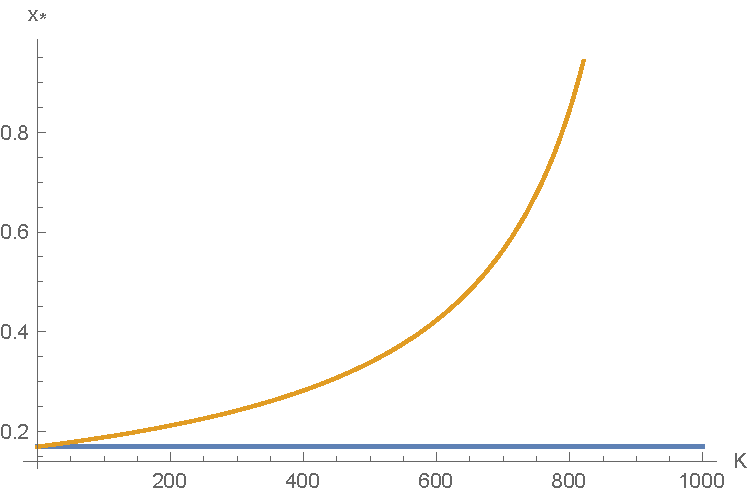
\includegraphics[width=0.45\textwidth]{Prob1_CapOpt/xopt_kvar.pdf}
	\caption{Threshold value with respect to the benchmark model (orange) and the capacity optimized model (blue), considering capacity levels $K \in [0, \theta/\alpha)$.}
	\label{fig:Kvar}
\end{figure}


On Figure \ref{fig:sigm} we observe that either for negative or positive values of the GBM's drift, both thresholds increase with volatility. This in accordance with \cite{rita} and \cite{hagspiel:cap} (VER CADERNO), whose works describe that with uncertainty is high, there is a delay time to invest, which is here reflected on an higher demand level.

\begin{figure}[!htb]
	\begin{subfigmatrix}{2}
		\subfigure[$\mu=-0.7$]{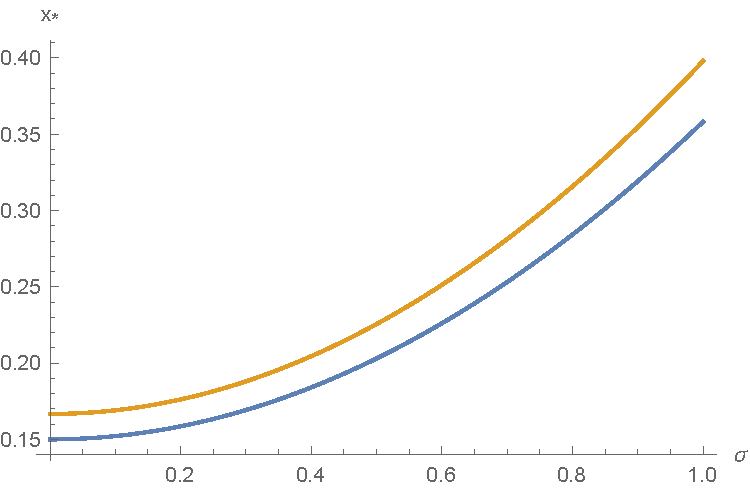
\includegraphics[width=0.45\textwidth]{Prob1_CapOpt/xopt_mu-7.pdf}}
			\subfigure[$\mu=0.03$]{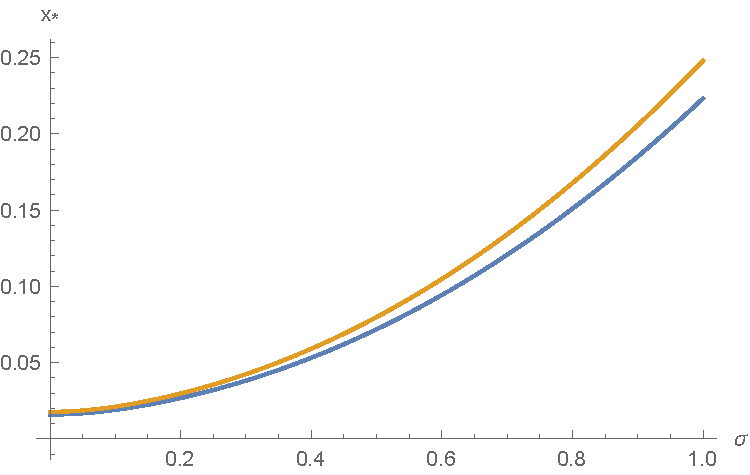
\includegraphics[width=0.45\textwidth]{Prob1_CapOpt/xopt_mu03.pdf}}
			\end{subfigmatrix}
			\caption{Threshold value with respect to the benchmark model (orange) and the capacity optimized model (blue), considering volatility $\sigma \in [0.0001, 1]$.}
			\label{fig:sigm}
\end{figure}

Regarding the drift parameter $\mu$ we obtained that the threshold values do not have a monotonic behaviour, either for smaller or bigger values of volatility. As showed in Figure \ref{fig:mu}, the smallest value of demand level necessary to invest is observed at the stationary point when $\mu=\sigma^2/2$.

\begin{figure}[!htb]
	\begin{subfigmatrix}{2}
		\subfigure[$\sigma=0.0001$]{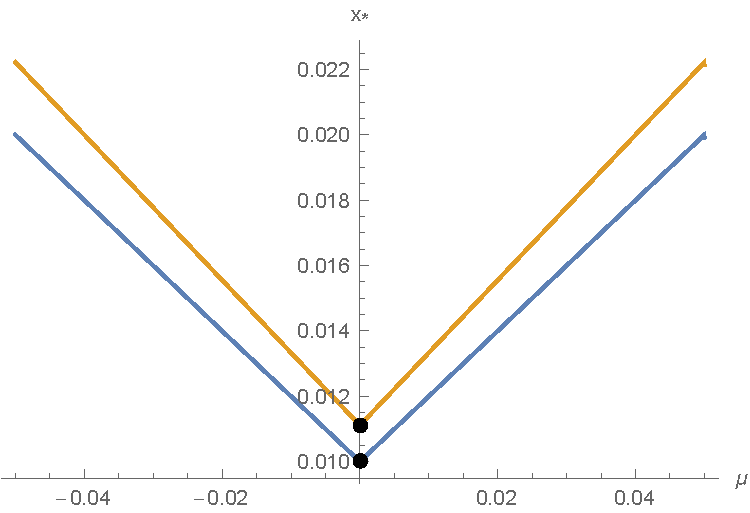
\includegraphics[width=0.45\textwidth]{Prob1_CapOpt/xopt_sigma0001.pdf}}
		\subfigure[$\sigma=0.3$]{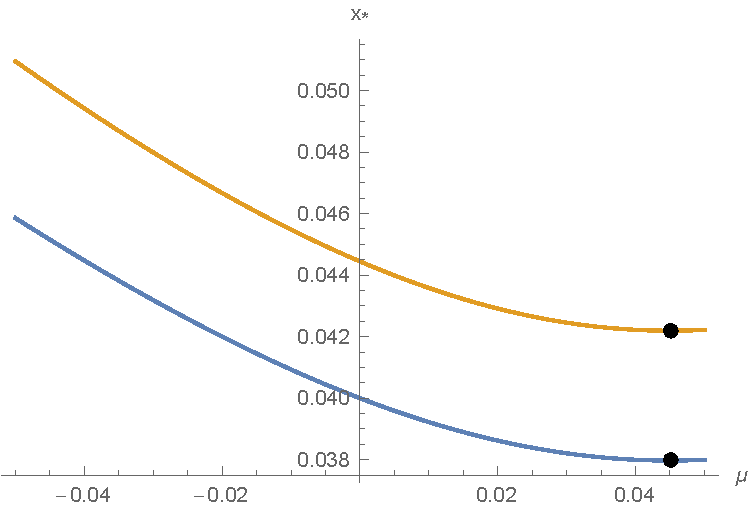
\includegraphics[width=0.45\textwidth]{Prob1_CapOpt/xopt_sigma3.pdf}}
	\end{subfigmatrix}
	\caption{Threshold value with respect to the benchmark model (orange) and the capacity optimized model (blue), considering drift $\mu \in [-r, r]$ and corresponding stationary point $\sigma^2/2$ (black).}
	\label{fig:mu}
\end{figure}

On Figure \ref{fig:td} we observe the behaviour of both threshold levels regarding the two other parameters, sensibility level $\delta$ and innovation level $\theta$. We have that the threshold levels increase with $\delta$ and decrease with $\theta$, as previously deduced.

\begin{figure}[!htb]
	\begin{subfigmatrix}{2}
	\subfigure[$\delta \in ( 0,10 )$ ]{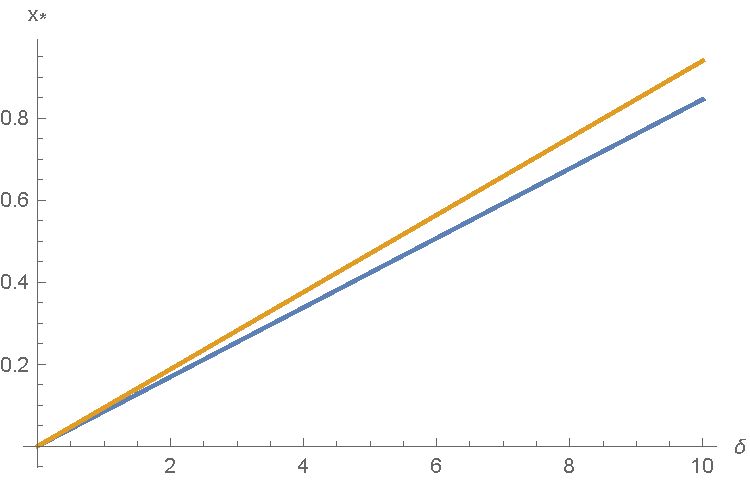
\includegraphics[width=0.45\textwidth]{Prob1_CapOpt/xopt_deltavar.pdf}}
	\subfigure[$\theta \in (\alpha K=1,50)$]{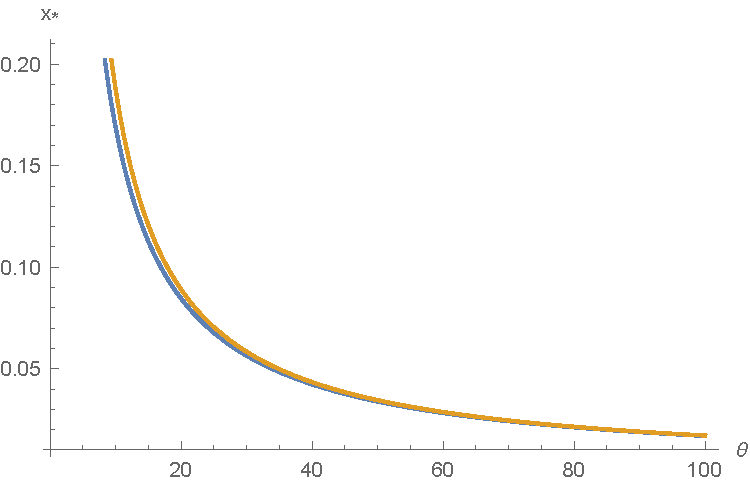
\includegraphics[width=0.45\textwidth]{Prob1_CapOpt/xopt_thetavar.pdf}}
	\end{subfigmatrix}
\caption{Threshold value with respect to the benchmark model (orange) and the capacity optimized model (blue), regarding sensibility parameter $\delta$ and innovation level $\theta$.}
\label{fig:td}
\end{figure}





Now we analyse optimal capacity level $K^*_C$, that is given by evaluating $K^*$ as defined in \eqref{} on demand level $x^*_C$, as done in \cite{huis:cap}. Its expression is given by
$$K^*_C=\frac{2 \sigma ^2 \theta}{\alpha \left(\sigma ^2 \left(\sqrt{\frac{4 \mu ^2}{\sigma ^4}-\frac{4 \mu }{\sigma ^2}+\frac{8 r}{\sigma ^2}+1}+3\right)-2 \mu \right)}.$$\\
\textbf{Proposition:}
Optimal capacity level $K^*_C$ increases with $\mu$, $\sigma$ and $\theta$ and decreases with $r$ and $\alpha$.

\textbf{Proof:}
The relation between $K^*_C$ and $\theta$, $r$ or $\alpha$ comes immediately by observing $K^*_C$ expression.

Now, regarding drift parameter we obtain that
 \begin{align*}
\frac{\partial K^*_C(\mu)}{\partial \mu}=
\frac{4 \theta \left(\sigma ^2 \left(\sqrt{\frac{4 \mu ^2}{\sigma ^4}-\frac{4 \mu }{\sigma ^2}+\frac{8 r}{\sigma ^2}+1}+1\right)-2 \mu \right)}{\alpha \sqrt{\frac{4 \mu ^2}{\sigma ^4}-\frac{4 \mu }{\sigma ^2}+\frac{8 r}{\sigma ^2}+1} \left(\sigma ^2 \left(\sqrt{\frac{4 \mu ^2}{\sigma ^4}-\frac{4 \mu }{\sigma ^2}+\frac{8 r}{\sigma ^2}+1}+3\right)-2 \mu \right)^2}>0.
\end{align*}
Since from
\begin{align}
\label{cond2}
\sigma ^2 \left(\sqrt{\frac{4 \mu ^2}{\sigma ^4}-\frac{4 \mu }{\sigma ^2}+\frac{8 r}{\sigma ^2}+1}+1\right)-2 \mu\geq0 
& \Leftrightarrow
\frac{4 \mu ^2}{\sigma ^4}-\frac{4 \mu }{\sigma ^2}+\frac{8 r}{\sigma ^2}+1 \geq \left( \frac{2 \mu}{\sigma^4}-1 \right)^2=\frac{4 \mu ^2}{\sigma ^4}-\frac{4 \mu }{\sigma ^2}+1 \\
& \Leftrightarrow
\frac{8 r}{\sigma ^2}\geq 0, \nonumber
\end{align}
which is true for $\forall r\geq 0$, and from \eqref{condd1} we obtain that both denominator and numerator are positive, from which the result comes.

Regarding volatility parameter we obtain that
 $$    \frac{\partial K^*_C(\sigma)}{\partial \sigma}= 
\frac{8 \theta \left(2 \mu ^2-\mu  \sigma ^2 \left(\sqrt{\frac{4 \mu ^2}{\sigma ^4}-\frac{4 \mu }{\sigma ^2}+\frac{8 r}{\sigma ^2}+1}+1\right)+2 r \sigma ^2\right)}{\alpha \sigma  \sqrt{\frac{4 \mu ^2}{\sigma ^4}-\frac{4 \mu }{\sigma ^2}+\frac{8 r}{\sigma ^2}+1} \left(\sigma ^2 \left(\sqrt{\frac{4 \mu ^2}{\sigma ^4}-\frac{4 \mu }{\sigma ^2}+\frac{8 r}{\sigma ^2}+1}+3\right)-2 \mu \right)^2}>0$$

From \eqref{demo} we obtain that the denominator is positive and from \eqref{condd1} and \eqref{cond2} that the denominator is positive for $\forall r\geq0$, from which the result holds.
\begin{flushright}
	$\square$
\end{flushright}


Considering some numerical approximations, we observe, on Figure \ref{fig:k1}, that $K^*_C$ increases with both drift and volatility. Note that, regarding the drift parameter, the growth is barely noticeable for negative values of $\mu$, but then it turns to be logarithmic. FINANCIAL INTERPRETATION? This seems to be related with the fact that for small drift values, the future expected demand value is smaller that for positive drift values. Recall that the demand process evolves accordingly to a GBM and its expected value at time $t$ is given by $\mathds{E} ^{X_0=x_0} [X_t]=x_0 e^{\mu t}$.

\begin{figure}[!htb]
	\begin{subfigmatrix}{2}
		\subfigure[$\mu \in ( -r,r )$ ]{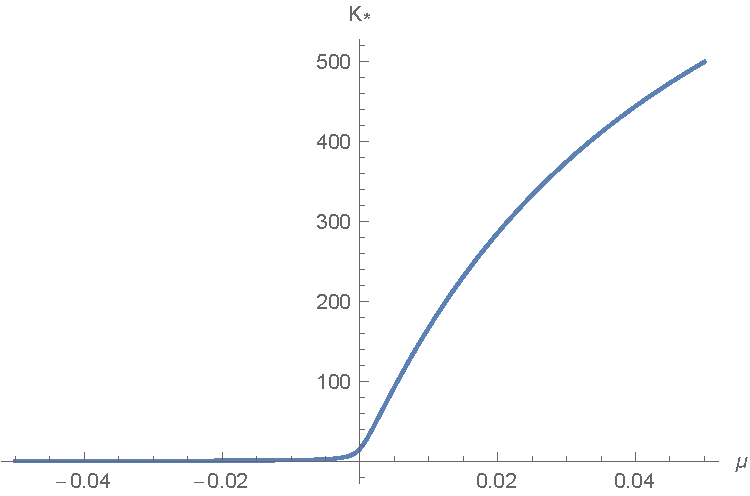
\includegraphics[width=0.45\textwidth]{Prob1_CapOpt/koptx_sigma005.pdf}}
		\subfigure[$\sigma \in (0,1)$]{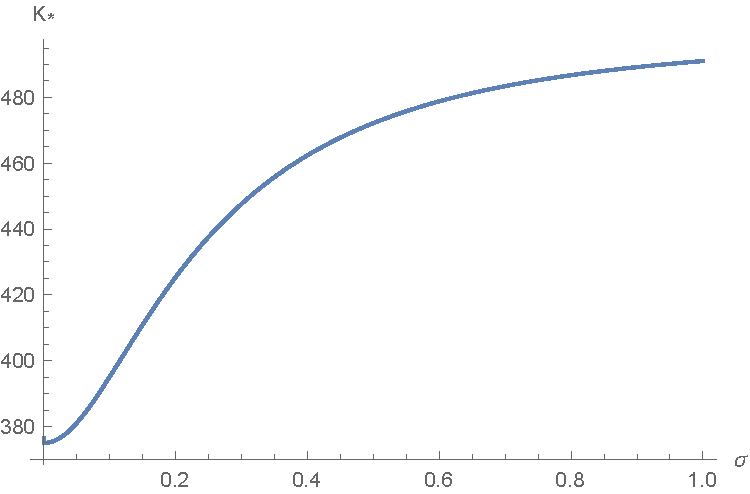
\includegraphics[width=0.45\textwidth]{Prob1_CapOpt/koptx_mu03.pdf}}
	\end{subfigmatrix}
	\caption{Optimal capacity regarding the threshold value $x^*_C$.}
	\label{fig:k1}
\end{figure}

Regarding discount rate $r$ and sensibility parameter $\alpha$, we have on Figure \ref{fig:k2} that $K^*_C$ decreases with them, as expected.
 
\begin{figure}[!htb]
	\begin{subfigmatrix}{2}
		\subfigure[$ r \in ( \mu, 1 )$]{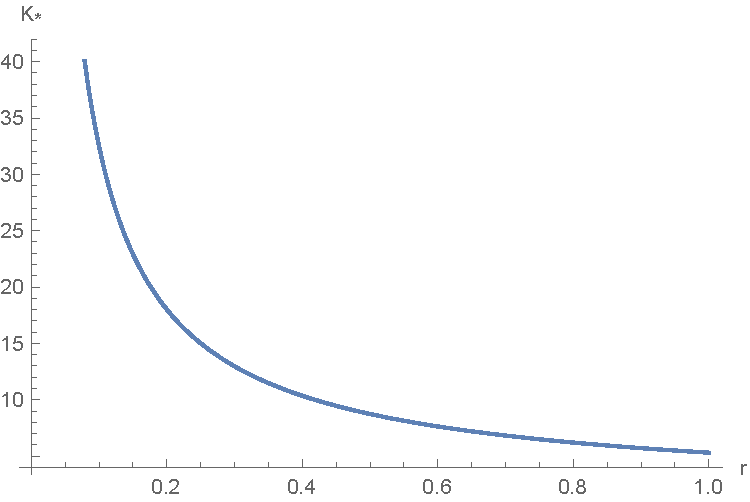
\includegraphics[width=0.45\textwidth]{Prob1_CapOpt/koptx_varr.pdf}}
		\subfigure[$ \alpha \in (0,1)$]{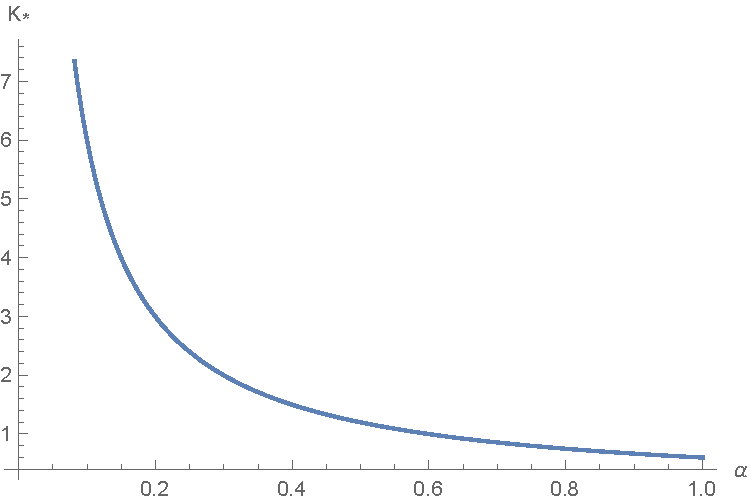
\includegraphics[width=0.45\textwidth]{Prob1_CapOpt/koptx_varalfa.pdf}}
	\end{subfigmatrix}
	\caption{Optimal capacity regarding the threshold value $x^*_C$.}
	\label{fig:k2}
\end{figure}









\subsection{R\&D and Capacity Optimization Model}
\label{subsec:RDcap1}

PASSOU PARA UM NOVO CAPÍTULO

As stated in section \ref{prob1max}, we are not able to solve analytically the polynomial presented in \eqref{} for every value $\gamma \in (0,1)$. However we considered some numerical approximations, using software \textit{Mathematica} and its function \texttt{Solve}. For the effect, we considered 
\begin{itemize}
	\item $r=0.05$;
	\item $F(X)=10$;
	\item $\gamma \in (0,1]$ incremented by 0.05.
\end{itemize}

Following results are implemented on script \texttt{RVopt.nb}.


\begin{figure}[!htb]
	\centering
	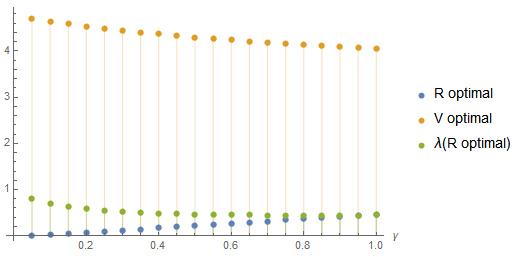
\includegraphics[width=0.6\textwidth]{Prob1_MaxProb/RVlambda_opt05.PNG}
	\caption{Optimal values of $R$ and $V(X)$ for fixed values of $F$ and $r$}
\end{figure}

We obtain that, although the optimal investment $R$ grows with exponent $\gamma$, the value function for the respective optimal $R$ decreases with exponent $\gamma$ (and in a different way from the decreasing of $\lambda(R)$). We get that the smaller value of $V(X)$ is approximately 4.05, corresponding to the optimal investment level $R=1$ and $\lambda(R)=0.45$ and the biggest value of $V(X)$ is approximately 4.69, corresponding to the optimal investment level $R=0.014$ and $\lambda(R)=0.05$ % file "Thesis_Background.tex"
\cleardoublepage

%%%%%%%%%%%%%%%%%%%%%%%%%%%%%%%%%%%%%%%%%%%%%%%%%%%%%%%%%%%%%%%%%%%%%%%%
%                                                                      %
%     File: Thesis_Results.tex                                         %
%     Tex Master: Thesis.tex                                           %
%                                                                      %
%     Author: Andre C. Marta                                           %
%     Last modified :  2 Jul 2015                                      %
%                                                                      %
%%%%%%%%%%%%%%%%%%%%%%%%%%%%%%%%%%%%%%%%%%%%%%%%%%%%%%%%%%%%%%%%%%%%%%%%

\chapter{Adding a new product when already producing one (Firm is already active before investing)}
\label{chapter:2}



%%%%%%%%%%%%%%%%%%%%%%%%%%%%%%%%%%%%%%%%%%%%%%%%%%%%%%%%%%%%%%%%%%%%%%%%
\section{Introduction}
\label{section:2_intro}

We consider now the case where, even before we decide to invest, the interested firm already produces a certain product. We also consider that the product is \textit{stable} in the market, in the sense that it's a recognized product, and so its demand function is not influenced by the demand level. Instead it's given by
$$p_0=1-\alpha K_0 $$
where $\alpha$ stands for a sensibility parameter and $K_0$ for the capacity of production of the \textit{old} product. 

However, the same is not valid for the new product. When the breakthrough takes place, the firm has the option to start to produce the new product. Since this one is a new product, susceptible to the consumers demand, its demand function is considered to be the same as in Section \ref{section:overview}, by the expression in \eqref{prob1:pi}, that is,
$$ p_1(X_t)=(\theta-\alpha K_1)X_t $$
where $\theta$ stands for the innovation level after the breakthrough, $\alpha$ for the same sensitivity parameter as in the \textit{old} product, $K_1$ for the capacity of production of the \textit{new} product and $X_t$ for the demand level at time $t$.

Recall that at the moment we decide to invest, we need to pay $\delta K_1$ related to sunk costs. 


As in the previous section, two models will be derived. The first one is the benchmark model. The second one consists in considering the maximized discount profit, associated with the investment decision, in terms of the capacity associated to the \textit{new} product.

%Here, as in Problem 1, we consider a unique possibly jump in the innovation process $\{ \theta_t, t \geq 0 \}$, that is denoted by $\theta$. 


%%%%%%%%%%%%%%%%%%%%%%%%%%%%%%%%%%%%%%%%%%%%%%%%%%%%%%%%%%%%%%%%%%%%%%%%
\section{Stopping Problem}
\label{section:2_theory}



\subsection{Benchmark Model}
\label{subsec:2_bm}

We want to find when is the best time to invest in the new product, knowing that the firm produces a \textit{stable}, that it's not influenced by the demand level and whose profit function is given by $\pi_0=p_0 K_0=(1-\alpha K_0)K_0$, and when the replacement happens, the firm will be immediately producing a product whose profit function is $\pi_1(X_t)=p_1(X_t) K_1 =(\theta-\alpha K_1)K_1 X_t$.

Thus our optimal stopping problem may be written as
\begin{equation}
\sup _\tau \textbf{E}^{X_0=x} \left[ \int_0^\tau \pi_0e^{-rs} ds + e^{-r\tau} \left( \int_\tau^\infty \pi_1(X_s)e^{-rs}ds -\delta K_1 \right) \right].
\label{eq:prob2}
\end{equation}

The first integral corresponds to the discounted profit obtain associated to the \textit{old} product from the time when the innovation level $\theta$ is reached until the time when the firm decides to invest in the \textit{new} product. The second integral corresponds to the discounted profit associated to the \textit{new} in the long term, after deciding to invest. Sutracting to it $\delta K_1)$, we obtain the profit associated to the investment decision, that to be evaluated in the precise time when the innovation breakthrough happens, must be discounted (multiplying the resultant expression by $e^{r \tau}$).

We can simplify this problem in order to have a standard optimal stopping problem with null running cost function.
Starting by conditioning \eqref{eq:prob2} to the time when the investment should happen and using Tower rule it follows that \eqref{eq:prob2} is equal to
\begin{equation}
\sup _\tau \textbf{E}^{X_0=x} \left[ \textbf{E}^{\tau=t} \left[  \int_0^\tau \pi_0e^{-rs} ds + e^{-r\tau} \left( \int_\tau^\infty \pi_1(x)e^{-rs}ds -\delta K_1 \right) \right] \right].
\label{eq:prob21}
\end{equation}

Since expectation is a linear operator, we can simplify each of the integrals separately.

Note that in the leftmost integral of \eqref{eq:prob21}, the instantaneous profit associated to the \textit{old} product does not depend on the demand level and all the parameters are deterministic. Then its expression can be simplified as
\begin{align}
\textbf{E}^{\tau=t} \left[\int_0^t \pi_0e^{-rs} ds \right] 
&= \textbf{E}^{\tau=t} \left[ \int_0^t p_0K_0e^{-rs} ds \right] \nonumber \\
&= \textbf{E}^{\tau=t} \left[ \int_0^t (1-\alpha K_0) K_0e^{-rs} ds \right] \nonumber \\
&= \textbf{E}^{\tau=t} \left[ (1-\alpha K_0) K_0 \frac{1-e^{-r t}}{r} \right] 
\label{g2}
\end{align}

Following a similar approach as in the previous section, when deducing \eqnref{prob1:h}, the leftmost expected value of the rightmost integral can also be simplified as

\begin{align}
\textbf{E}^{\tau=t} \left[  \int_t^\infty \pi_1(X_s)e^{-rs} ds -\delta K_1 \right]
&=  \textbf{E}^{\tau=t} \left[  \int_t^\infty p_1(X_s) K_1e^{-rs} ds -\delta K_1 \right] \nonumber \\
&= \textbf{E}^{\tau=t} \left[ \int_t^\infty (\theta-\alpha K_1)X_s K_1e^{-rs} ds -\delta K_1 \right] \nonumber \\
&= \textbf{E}^{\tau=t} \left[\frac{(\theta-\alpha K_1)K_1 x_\tau}{r-\mu} -\delta K_1 \right] 
\label{h2}
\end{align}
where $x_\tau$ is taken to be the observed demand level at the time when the \textit{new} product starts being produced. Recall, fromthe previous section, that expression \eqref{h2} only holds if the assumptions of Fubini's Theorem hold, that is $r-\mu>0$.

Denote $F$ as the value function solution to \eqref{eq:prob21}. Plugging expressions \eqref{g2} and \eqref{h2} in \eqref{eq:prob21}, getting rid of the expectation conditional to time when the investment decision is made, using (again) Tower rule, we obtain that $F$ may be written as

\begin{equation}
F(x)=\frac{\pi_0}{r}+ \sup _\tau \textbf{E}^{X_0=x} \left[ e^{-r\tau}\left(\frac{(\theta-\alpha K_1)K_1 X_\tau}{r-\mu} - \left( \delta K_1  +\frac{\pi_0}{r}\right)  \right) \right],
\label{prob235}
\end{equation}
which corresponds to the sum of a constant term with a standard optimal stopping problem with null running cost function, as we wanted. This is the effect of dealing with a very stable product, which doesn't depend on the current demand level, allowing us to simply this much its expression.

Note that the terminal cost function here, given by $h(x)=\frac{(\theta-\alpha K_1)x}{r-\mu} - \left( \delta K_1  +\frac{(1-\alpha K_0) K_0}{r}\right)$, is a non-decreasing function in $x$ of the type $h(x,\underline{\psi})=k(\underline{\psi})x-j(\underline{\psi})$ with $k(\underline{\psi})$ and $j(\underline{\psi}) > 0$ functions, $\underline{\psi}$  a vector corresponding to the deterministic arguments and $x$ corresponding to the stochastic argument.

Considering $V$ to be the optimal standard problem present in \eqref{prob235}, that is
\begin{equation}
V(x)=  \sup _\tau \textbf{E}^{X_0=x} \left[ e^{-r\tau}h(X_\tau) \right] 
=\sup _\tau \textbf{E}^{X_0=x} \left[ e^{-r\tau}\left(\frac{(\theta-\alpha K_1)K_1 X_\tau}{r-\mu} - \left( \delta K_1  +\frac{\pi_0}{r}\right)  \right) \right],
\end{equation} 
$V$ must verify the HJB variational inequality \eqref{HJB}. As was written in Section , $V$ must then be of the form
\begin{equation}
V(x)=\begin{cases} a_2(x^*)^{d_1} \ , \ x \in \mathcal{C} \\
\frac{(\theta-\alpha K_1)K_1 X_\tau}{r-\mu} - \left( \delta K_1  +\frac{\pi_0}{r}\right)=\frac{K(\theta-\alpha K)}{r-\mu} \ , \ x \in \mathcal{S}
\end{cases}
\end{equation}
and must verify value matching and smooth pasting conditions, leading to the system
\begin{equation}
\begin{cases} a_2(x^*)^{d_1}=\frac{(\theta-\alpha K_1)K_1 X_\tau}{r-\mu} - \left( \delta K_1  +\frac{\pi_0}{r}\right)=\frac{K(\theta-\alpha K)}{r-\mu} \\
a_2d_1(x^*)^{d_1-1}=\frac{K(\theta-\alpha K)}{r-\mu},
\end{cases}
\label{eq:sistema2}
\end{equation}
By the system above and according to \ref{satz}, the threshold  $x^*$ and the coefficient $a_2$ are respectively given by
\begin{align}
&x^*=\frac{d_1}{d_1-1} \frac{ \delta K_1  +\frac{1-\alpha K_0}{r}K_0 }{\theta-\alpha K_1} \frac{r-\mu}{K_1} \\
&a_2=\left( \delta K_1 +\frac{1-\alpha K_0}{r}K_0 \right) \frac{(x^*)^{-d_1}}{d_1-1} \nonumber.
\end{align}

Plugging the results stated above on the expression of $F$ \eqref{prob235}, it leads to
\begin{equation}
F(x)=\frac{\pi_0}{r}+\begin{cases} a_2(x^*)^{d_1} \ , \ x \in \mathcal{C} \\
\frac{(\theta-\alpha K_1)K_1 X_\tau}{r-\mu} - \left( \delta K_1  +\frac{\pi_0}{r}\right)=\frac{K(\theta-\alpha K)}{r-\mu} \ , \ x \in \mathcal{S},
\end{cases}
\end{equation}
where the continuation and stopping regions associated to this problem are given by
$$\mathcal{C}=\left\{ x \in \textbf{R}^+: x \leq x^* = \frac{d_1}{d_1-1} \frac{ \delta K_1  +\frac{1-\alpha K_0}{r}K_0 }{\theta-\alpha K_1} \frac{r-\mu}{K_1} \right\}$$
$$\mathcal{S}=\textbf{R}^+ \setminus \mathcal{C}= \left\{ x \in \textbf{R}^+: x > x^* =\frac{d_1}{d_1-1} \frac{ \delta K_1  +\frac{1-\alpha K_0}{r}K_0 }{\theta-\alpha K_1} \frac{r-\mu}{K_1} \right\}.$$
and the stopping time referred in \eqref{prob235}, corresponding the optimal time when the investment decision should be made, is formally defined as $\tau=\inf\{t\geq0: X(t) \in \mathcal{S} \}=\inf\{t\geq 0: X(t) \geq x^* \}$.




\subsection{Capacity Optimization Model}
\label{subsec:2_com}



%\section{Maximization Problem}


\section{Comparative Statics}
Since the obtained results cannot reduce to each other, as done in the previous section, we will treat each case separately, starting with the simplest one derived in \ref{subsec:2_bm}.
Comparisons between the benchmark and capacity optimization models will be made on subsection 3.4.2.\\

\subsection{Benchmark Model}
%In this section we study the behaviour of the decision threshold $x^*_B$ and $x^*_{C}$ and $K^*$ as described in \eqref{ass3}, with the different parameters.


\textbf{Proposition:}
Decision threshold $x^*_B$ increases with $ \delta, \ \sigma$ and $\alpha$ only when $\theta < \frac{K_1}{ K_0^2} (K_0+K_1 r \delta)$, decreases with $\theta$ and $\alpha$ only when $\theta > \frac{K_1}{ K_0^2} (K_0+K_1 r \delta)$ and does not have a monotonic behaviour with $K_0, \ K_1, \ r$.


\textbf{Proof:}

Regarding the formula obtained for  $x^*_B$, we immediately conclude that the decision threshold increases with $\delta$ and decreases with $\theta$.

Regarding $\sigma$, we observe that


$$    \frac{\partial x^*_B ( \sigma ) }{\partial \sigma}= 
\frac{(r-\mu )  \left(\delta  K_1+\frac{K_0(1-\alpha K_0)}{r}\right)}{(d_1-1) K_1 (\theta -\alpha  K_1)} \left(\frac{2 \mu }{\sigma ^3}+\frac{\frac{4 \mu  \left(\frac{1}{2}-\frac{\mu }{\sigma ^2}\right)}{\sigma ^3}-\frac{4 r}{\sigma ^3}}{2 \sqrt{\left(\frac{1}{2}-\frac{\mu }{\sigma ^2}\right)^2+\frac{2 r}{\sigma ^2}}}\right) \left( 1- \frac{d_1}{(d_1^2-1} \right).$$


Taking into account our initial assumptions about $r, \ \mu$ and profits associated to the old and the new product, it follows that the leftmost expression is always positive. Since $d_1^2-d_1+1>0 \ \ \forall d_1$, the rightmost expression is also positive. Now we need to analyse the expression in between. We chec

Problemas em mostrar quando é que a segunda derivada é positiva.

Regarding $K_0$, we observe that

\begin{align*}
\frac{\partial x^*_B ( K_0 ) }{\partial K_0}= 
\frac{d_1 (r-\mu )}{r (d_1-1)K_1(\theta-\alpha K_1)} (1-2\alpha K_0)
=
\begin{cases}
>0 &\ \text{for} \ K_0<\frac{1}{2 \alpha}\\
<0 &\ \text{for} \ K_0>\frac{1}{2 \alpha}
\end{cases}.
\end{align*}
since the expression represented in fraction is always positive.


Regarding $K_1$, we obtain that

\begin{align*}
\frac{\partial x^*_B ( K_1 ) }{\partial K_1}= 
\frac{d_1 (r-\mu )}{ (d_1-1)K_1(\theta-\alpha K_1)}  \left( \frac{\alpha (\frac{K_0(1-\alpha K_0)}{r}+K_1 \delta )}{\theta-\alpha K_1} -\frac{ \frac{K_0(1-\alpha K_0)}{r}+K_1 \delta )}{K_1}+ \delta \right)
\end{align*}


The leftmost expression is always positive. Thus we only need to evaluate the sign of the expression next to it. Manipulating mentioned expression, taking into account that the capacity level cannot be negative as well as the price function given by $\pi_0=K_0(1-\alpha K_0)$, it follows that

\begin{align*}
\frac{\partial x^*_B ( K_1 ) }{\partial K_1}= 
\begin{cases}
>0 &\ \text{for} \ K_1>\frac{-\pi_0+\sqrt{\alpha \pi_0 (\pi_0 + r \delta \theta)}}{ r\alpha \delta}\\
<0 &\ \text{for} \ K_1 \in \left[ 0, \frac{-\pi_0+\sqrt{\alpha \pi_0(\pi_0 + r \delta \theta)}}{ r\alpha \delta} \right]
\end{cases},
\end{align*}
from which we obtain that $x^*_B$ has no monotonic behaviour with $K_1$.


Regarding parameter $\alpha$, we obtain that

\begin{align*}
\frac{\partial x^*_B ( \alpha ) }{\partial \alpha}= 
\frac{d_1 (r-\mu )}{ (d_1-1)(\theta-\alpha K_1)}  \left( \frac{\frac{K_0(1-\alpha K_0)}{r}+ \delta K_1  }{\theta-\alpha K_1} -\frac{ K_0^2}{r K_1} \right),
\end{align*}
where the leftmost expression is always positive. Simplifying the expression in the biggest brackets to the same denominator, we obtain that
\begin{align*}
\frac{\partial x^*_B ( \alpha ) }{\partial \alpha}= 
\begin{cases}
>0 &\ \text{for} \ \theta < \frac{K_0 K_1 +K_1^2 r\delta}{K_0^2}\\
<0 &\ \text{for} \ \theta > \frac{K_0 K_1 +K_1^2 r\delta}{K_0^2}.
\end{cases}
\end{align*}

Note that the sign of the partial derivative does not depend on $\alpha$.

Regarding parameter $r$ we obtained complex derivates, from which we weren't able to deduce any analytical results. However, as it will be showed right after this proof, using Mathematica we obtained that $x^*_B$ behaves in a non-monotonic way with it.

\begin{flushright}
	$\square$
\end{flushright}

We weren't able to deduce any analytical result regarding the drift value $\mu$. However, after many numerical experiments, we observed that $x_B^*$ decreases with $\mu$, as it's showed on Figure \ref{fig:2_x3}.


\subsection{Capacity Optimization Model}

\textbf{Proposition:}
Decision threshold $x^*_C$ increases with $\delta$, decreases asymptotically with $\theta$ and do not have a monotonic behaviour with $\mu, \ r, \alpha, K_0$.


\textbf{Proof:}

For the sake of simplicity, we will denote, in this proof, 
$\phi:=\sqrt{\frac{4 \mu ^2}{\sigma ^4}-\frac{4 \mu }{\sigma ^2}+\frac{8 r}{\sigma ^2}+1}>0$ and
$\psi:=4 d_1^2 \pi_0  (\delta  \theta  r+\pi_0 )+\delta ^2 \theta ^2 r^2>0$.
Recall also that $\pi_0>0$ stands for the profit function associated to the new product.

Regarding $\delta$, we obtain that

\begin{align*}
\frac{\partial x^*_B ( \delta ) }{\partial \delta}= \frac{(r-\mu ) \left(\frac{4 d_1^2 \theta  r \pi_0 +2 \delta  \theta ^2 r^2}{2 \sqrt{\psi }}+d_1 \theta  r\right)}{(d_1-1) \theta ^2 r}>0
\end{align*}
from which the result holds.

Regarding $\theta$, we obtain that

\begin{align*}
\frac{\partial x^*_B ( \theta) }{\partial \theta}= \frac{ \theta (r-\mu ) \left(\frac{4 \delta  d_1^2 r \omega +2 \delta ^2 \theta  r^2}{2 \sqrt{\psi }}+\delta  d_1 r\right)- 2 (r-\mu ) \left(d_1 (\delta  \theta  r+2 \omega )+\sqrt{\psi }\right)}{(d_1-1) \theta ^3 r}.
\end{align*}

Manipulating the numerator, it simplifies to
$$
\frac{\delta  d_1 r \left(2 d_1 (1-4 \theta ) \omega +(1-2 \theta ) \sqrt{\psi }\right)-4 d_1 \omega  \left(2 d_1 \omega +\sqrt{\psi }\right)+\delta ^2 \theta ^2 \left(-r^2\right)}{\sqrt{\psi}}$$
which is always negative for innovation levels $\theta>1/2$. COMPLETAR: ARRANJAR SUPOSIÇÃO MAIS FORTE

Since we assume that innovation levels have no upper limit, we evaluated them asymptotically. Denoting $\theta_A:=\frac{(r-\mu )}{(d_1-1) r}  \left(\sqrt{\delta ^2 r^2}+\frac{\delta  r \left(\sigma ^2 (\phi +1)-2 \mu \right)}{2 \sigma ^2}\right)>0$ we obtain that $x^*_C$ decreases on order of $\frac{\theta_A}{\theta}$, that is,  

$$x^*_C(\theta) \sim \frac{\theta_A}{\theta} \ \Leftrightarrow \ \lim_{\theta \to \infty} \frac{x^*_C(\theta)}{\frac{\theta_A}{\theta}}=1.$$

Regarding parameters $\mu$, $r$ $\alpha$ and $K_0$, we obtained complex derivates, from which we couldn't deduce any analytical result. However, as it will be showed hereunder, $x^*_C$ behaves in a non-monotonic way with all of them.
\begin{flushright}
	$\square$
\end{flushright}


Although we couldn't obtain any analytical (strong) evidence, after different experiments done using \textit{Mathematica} and its function \texttt{Manipulate}, we obtained that decision thresholds $x^*_B$ and $x^*_C$ increase with volatility $\sigma$. An example is showed on Figure \ref{fig:2_x2}.



To illustrate results above mentioned we performed some numerical illustrations, using software \textit{Mathematica} and its function \texttt{Manipulate}. However here are only able to present static plots - we leave to the interested ones, to see the results achieved with \texttt{Manipulate}.

Unless it is written the opposite, following values were considered:
\begin{table*}[!htb]
	\centering
	%\label{my-label}
	\begin{tabular}{lllllll}
		$\bullet$ & $\mu=0.03$     &  & \hspace{7cm} &  &  $\bullet$ & $\alpha=0.01$ \\
		$\bullet$ & $\sigma=0.005$ &  & \hspace{7cm} &  &  $\bullet$ & $\theta=10$   \\
		$\bullet$ & $r=0.05$       &  & \hspace{7cm} &  &  $\bullet$ & $K_0=90$       \\
		$\bullet$ & $\delta=2$     &  & \hspace{7cm} & &  $\bullet$ & $K_1=100$                                   
	\end{tabular}
	%\caption{bjde}
\end{table*}

%\begin{itemize}
%		\item $\mu=0.03$
%		\item $\sigma=0.005$ 
%		\item $r=0.05$
%		\item $\delta=2$
%		\item $\alpha=0.01$
%		\item $\theta=10$
%		\item $K=100$	
%\end{itemize}


%We start by illustrating how does $x^*_B$ and $x^*_C$ are related by the capacity level $K$, on which $x^*_B$ is dependent. One can see on Figure \ref{fig:Kvar} that conclusions mentioned on the proof (including that $x^*_B(0)=x^*_C$) hold.


\begin{figure}[!htb]
	\begin{subfigmatrix}{2}
		\subfigure[$\delta \in (0,1)$]{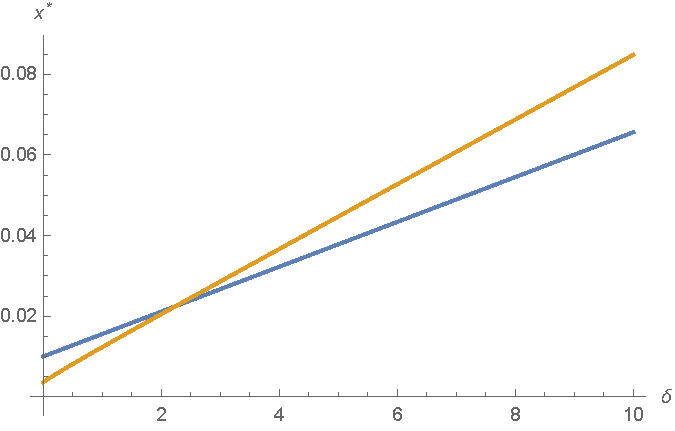
\includegraphics[width=0.45\textwidth]{Prob2_CapOpt/xopt_delta.pdf}}
		\subfigure[$\sigma \in (0,1)$]{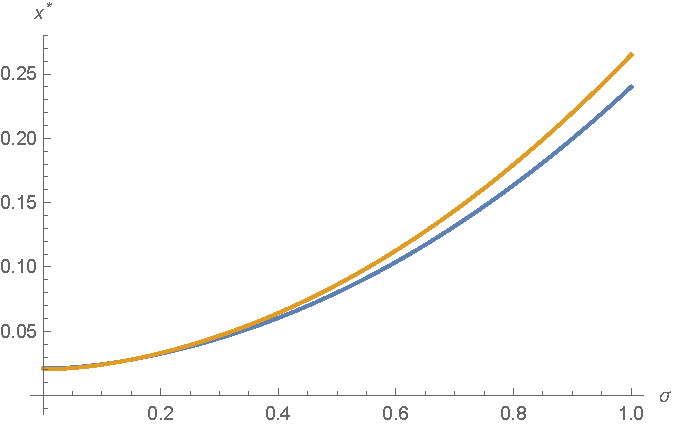
\includegraphics[width=0.45\textwidth]{Prob2_CapOpt/xopt_sigma.pdf}}
	\end{subfigmatrix}
	\caption{Threshold value with respect to the benchmark model (orange) and the capacity optimized model (blue) and parameters with which $x^*_B$ increases.}
	\label{fig:2_x2}
\end{figure}

On Figure \ref{fig:2_x2}, we obtained similar results to the ones on Section 2. Both threshold values increase with sensibility parameter $\delta$ and volatility $\sigma$. The first one is justified by the fact that a higher $\delta$ means a bigger investment, and thus it will only be made, if there's also a huge demand of the product. The second one is justified by the huge uncertainty of the demand. Since it has a high variance, the demand has a great amplitude of values, which delays the investment decision, only made when the demand reaches a high level. This is in accordance to what is described in \cite{dixit:book}.


\begin{figure}[!htb]
	\begin{subfigmatrix}{2}
		\subfigure[$\mu \in ( -r,r )$ ]{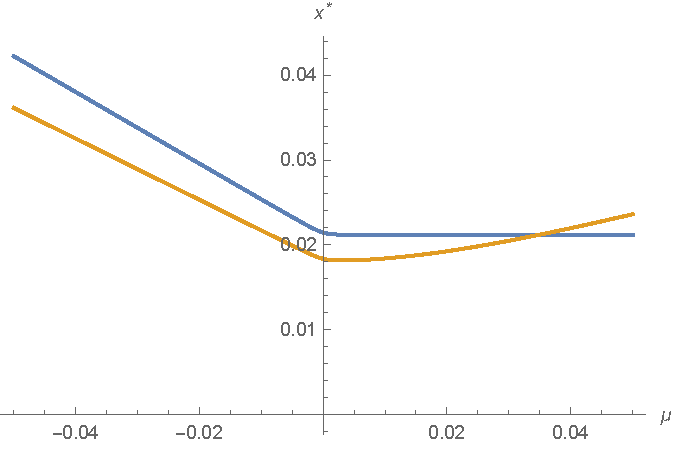
\includegraphics[width=0.45\textwidth]{Prob2_CapOpt/xopt_mu.pdf}}
		\subfigure[$\theta \in (1,10)$]{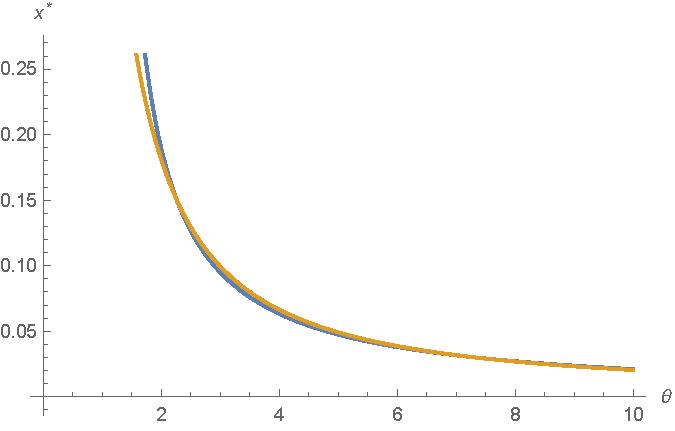
\includegraphics[width=0.45\textwidth]{Prob2_CapOpt/xopt_theta.pdf}}
	\end{subfigmatrix}
	\caption{Threshold value with respect to the benchmark model (orange) and the capacity optimized model (blue) and parameter with which  $x^*_B$ decreases.}
	\label{fig:2_x3}
\end{figure}

On Figure \ref{fig:2_x3} we see that similarly to what happened on Section 2, both threshold levels decrease with innovation level. Although the threshold level associated to the benchmark model decreases with $\mu$ in what seems to be a linear way for negative values of $\mu$ and almost negligible for positive values of $\mu$, the same doesn't happen to the threshold level associated to the capacity optimization model. This last one, seems to increase for positive values of $\mu$. The same happened considering other values for parameters $K_0, \ \alpha, \ \delta, \ \theta$. Regarding $\sigma$, we obtained that when increasing the volatility, the value of $\mu$ associated wityh the stationary point happens for values of $\mu$ greater than 0.

\begin{figure}[!htb]
	\begin{subfigmatrix}{2}
		\subfigure[$r \in (\mu,1)$, $\mu=0.01$ and $\sigma=0.9$]{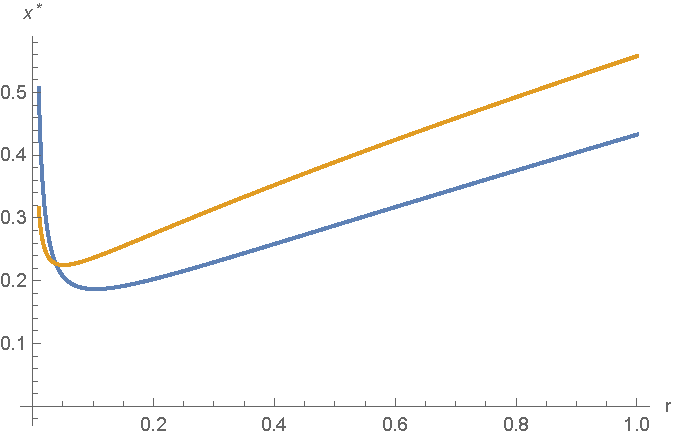
\includegraphics[width=0.45\textwidth]{Prob2_CapOpt/xopt_r.pdf}}
		\subfigure[$K_0 \in ( 0, \frac{1}{\alpha}=100 )$ ]{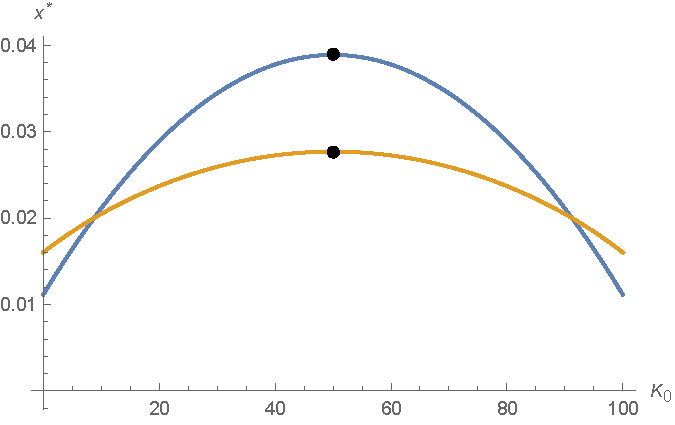
\includegraphics[width=0.45\textwidth]{Prob2_CapOpt/xopt_k0.pdf}}
		\subfigure[$K_1 \in (0, \frac{\theta}{\alpha}=1000 )$]{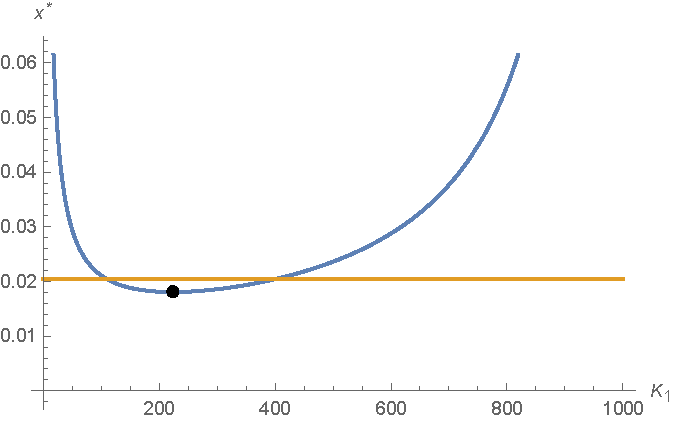
\includegraphics[width=0.45\textwidth]{Prob2_CapOpt/xopt_k1.pdf}}
	\end{subfigmatrix}
	\caption{Threshold value with respect to the benchmark model (orange) and the capacity optimized model (blue) and parameters with which  $x^*_B$ has a non-monotonic behaviour.}
	\label{fig:2_x1}
\end{figure}

On Figure \ref{fig:2_x1}, we observe that both threshold level behave in a non-monotonic way with $r$ and $K_0$.

Interestingly, a maximum value is observed when the capacity level of the \textit{older} product is exactly equal to $\frac{1}{2 \alpha}$, whose value comes from the expression $\alpha K_0 \pi_0=\alpha K_0 (1-\alpha K_0)$ included on both expressions of $x_B^*$ \eqref{} and $x^*_C$ \eqref{}.

Regarding parameter $K_1$, its value doesn't affect threshold $x^*_C$, since it takes into account the optimal capacity $K^*_C$. However, when it comes to the threshold $x^*_B$ we have that it achieves a minimum value at $K_1=\frac{\pi_0+\sqrt{\alpha \pi_0(\pi_0+\delta \theta r)}}{r\alpha \delta}$, as it's represented on the bottom plot.
	
	\begin{figure}[!htb]
		\begin{subfigmatrix}{2}
			\subfigure[$\alpha \in (0,1)$$\theta=10>\frac{K_1}{ K_0^2} (K_0+K_1 r \delta)$]{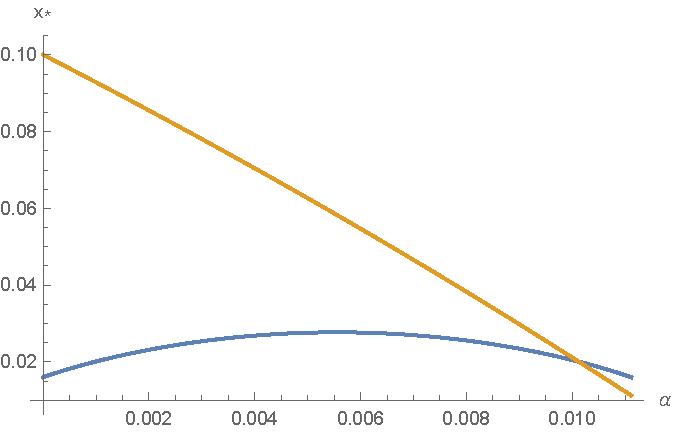
\includegraphics[width=0.45\textwidth]{Prob2_CapOpt/xopt_alpha.pdf}}
			\subfigure[$\alpha \in (0,1) $ and $\theta=1<\frac{K_1}{ K_0^2} (K_0+K_1 r \delta)$]{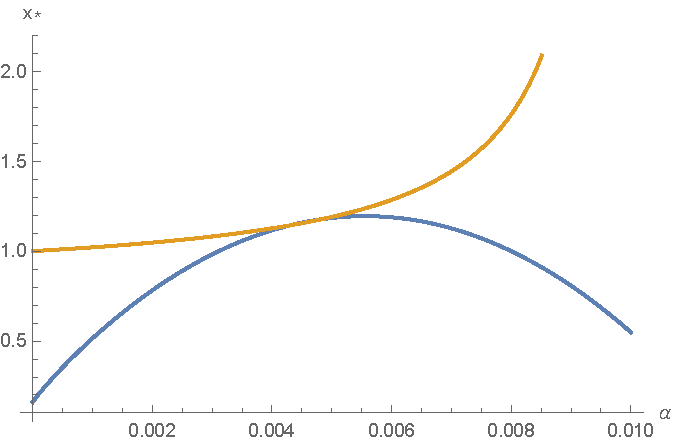
\includegraphics[width=0.45\textwidth]{Prob2_CapOpt/xopt_alpha_o1.pdf}}
		\end{subfigmatrix}
		\caption{Threshold value with respect to the benchmark model (orange) and the capacity optimized model (blue) and sensibility parameter $\alpha$.}
		\label{fig:2_x4}
	\end{figure}
	
	On Figure \ref{fig:2_x4} it's represented the behaviour of $x^*_B$ with $\alpha$, as written on Proposition (???). Considering fixed values mentioned in REFERIRRRR, we obtain a $\theta$-threshold equal to $\frac{K_1}{ K_0^2} (K_0+K_1 r \delta)=1.23457$. Testing for innovation levels smaller and greater than the mentioned threshold, we verify what was deduced: that $x^*_C$ behaves differently with $\alpha$ for certain levels of innovation.
	
	Note that on most of the plots you have that the threshold $x_C^*$ has an associated capacity level ($K^*(x_C^*)$) greater than the one considered ($K_1=100$), resulting in values $x^*_B$ smaller than $x_C^*$, contrarily to what happened on the previous section.
	\vspace{2cm}
	
	Now we analyse optimal capacity level $K^*_C$, that is given by evaluating $K^*$ as defined in \eqref{ass3} on demand level $x^*_C$, as done in \cite{huis:cap} and in the previous section. Its expression is given by
$$K^*_C=\frac{\theta }{2 \alpha }-\frac{\delta  (d_1-1) \theta ^2 r}{2 \alpha  \left(\sqrt{4 \alpha  d_1^2 \pi_0 (\alpha  \pi_0+\delta  \theta  r)+\delta ^2 \theta ^2 r^2}+d_1 (2 \alpha  \pi_0+\delta  \theta  r)\right)}.$$\\

\textbf{Proposition:}
Optimal capacity level $K^*_C$ increases asymptotically with $\theta$ and does not have a monotonic behaviour with $K_0$. Also, 

\textbf{Proof:}

Regarding innovation level $\theta$, assuming that it has no upper limit, it's possible to evaluate its behaviour asymptotically. Denoting $\theta_K:=\frac{\sigma ^2 \left(\sqrt{\delta ^2 r^2}+\delta  r\right)}{\alpha  \left(2 \sigma ^2 \sqrt{\delta ^2 r^2}+\delta  r \left(\sigma ^2 (\phi +1)-2 \mu \right)\right)}>0$, we obtain that $K^*_C$ increases on order of $\theta_K \theta$, that is,
$$K^*_C(\theta) \sim \theta_K \theta \ \Leftrightarrow \ \lim_{\theta \to \infty}  \frac{K^*_C}{\theta_K \theta}=1 $$


The non monotonic behaviour of $K^*_C$ with $K_0$ will be showed hereunder in the obtained plots.
\begin{flushright}
	$\square$
\end{flushright}

Although it wasn't possible to derive any (strong) analytical solution about te behaviour of the other parameters, numerically we obtain robust results. By manipulating each parameter, using command \texttt{Manipulate}, we obtained no different behaviours from the ones showed hereunder.

The results obtained regarding parameters $\mu, \ \sigma,\ r, \ \alpha$ and $\theta$  were similar to the ones obtain for the optimal capacity level on the previous section.  Since $K^*_C$ depends on value $x_C^*$, it is expected to observe similiar behaviours regarding the studied parameters. 

Starting with the capacity level of the \textit{old} product $K_0$ and respective considered parameters, on Figure \ref{fig:2_k0}, we obtained that the highest optimal capacity level $K^*_C$ happens for $K_0=\frac{1}{2 \alpha}$. This is motivated by the results obtained for $x^*_C$, as seen on Figure \ref{fig:},which also reaches its highest value at $\frac{1}{2 \alpha}$.

\begin{figure}[!htb]
	\centering
	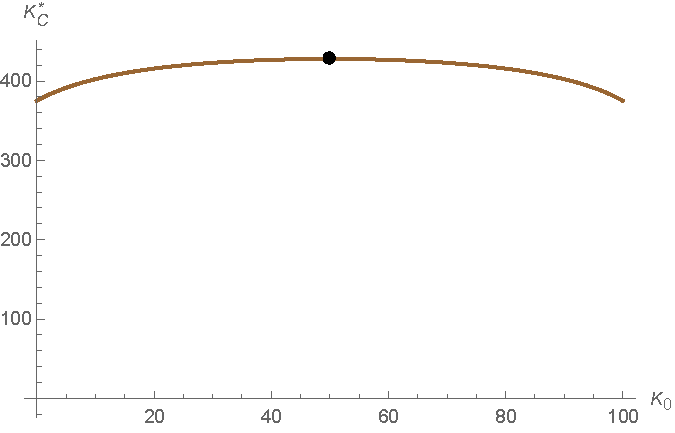
\includegraphics[width=0.45\textwidth]{Prob2_CapOpt/koptx_k0.pdf}
	\caption{Optimal capacity regarding the threshold value $x^*_C$ considering capacity levels $K_0 \in [0, 100)$ and its highest values at $\frac{1}{2 \alpha}=50$.}
	\label{fig:2_k0}
\end{figure}

On Figure \ref{fig:2_k1}, we obtain that $K^*_C$ increases with both drift and volatility, as it happened in the previous section. Note that again that, contrary to what happens for positive drift values, the growth of $K^*_C$ with $\mu$ is barely noticeable for negative values of $\mu$.
%Recall that the demand process evolves accordingly to a GBM and its expected value at time $t$ is given by $\textbf{E}^{X_0=x_0} [X_t]=x_0 e^{\mu t}$.

\begin{figure}[!htb]
	\begin{subfigmatrix}{2}
		\subfigure[$\mu \in ( -r,r )$ ]{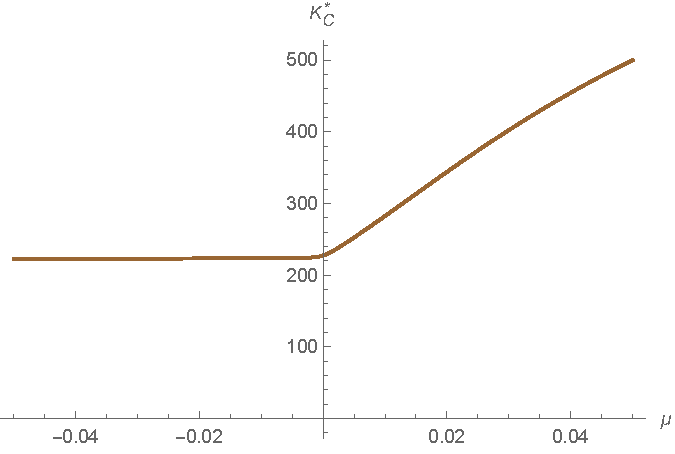
\includegraphics[width=0.45\textwidth]{Prob2_CapOpt/koptx_mu.pdf}}
		\subfigure[$\sigma \in (0,1)$]{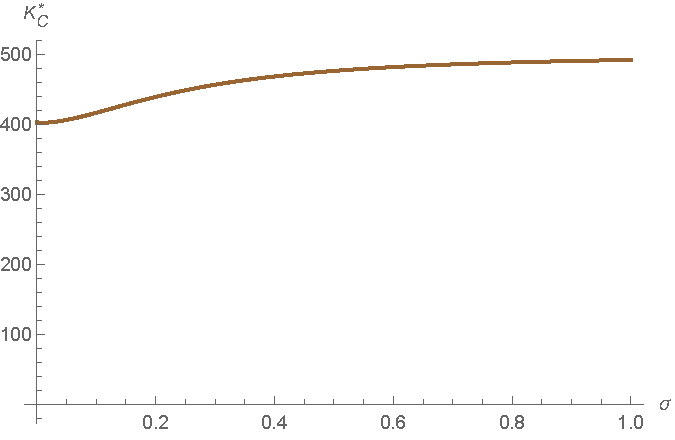
\includegraphics[width=0.45\textwidth]{Prob2_CapOpt/koptx_sigma.pdf}}
	\end{subfigmatrix}
	\caption{Optimal capacity regarding the threshold value $x^*_C$.}
	\label{fig:2_k1}
\end{figure}

Regarding innovation level $\theta$ and sensibility parameter $\delta$, we have on Figure \ref{fig:2_k3} that $K^*_C$ increases with them as well. Note that asymptotically, $K^*_C$ seems to increase linearly with $\theta$, as previously deduced.

\begin{figure}[!htb]
	\begin{subfigmatrix}{2}
		\subfigure[$ \theta \in ( 1, 10 )$]{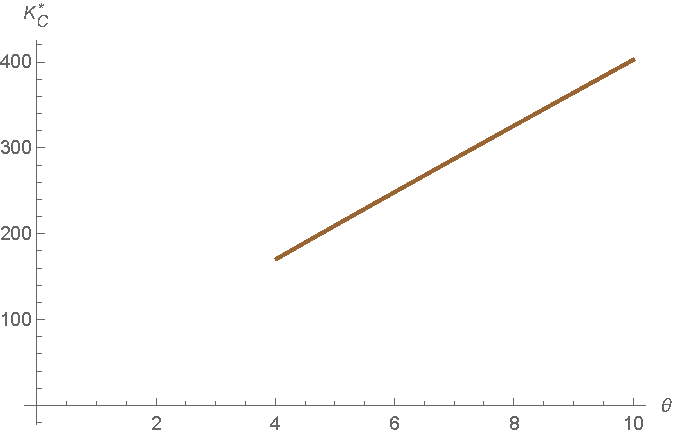
\includegraphics[width=0.45\textwidth]{Prob2_CapOpt/koptx_theta.pdf}}
		\subfigure[$ \delta \in (0,10)$]{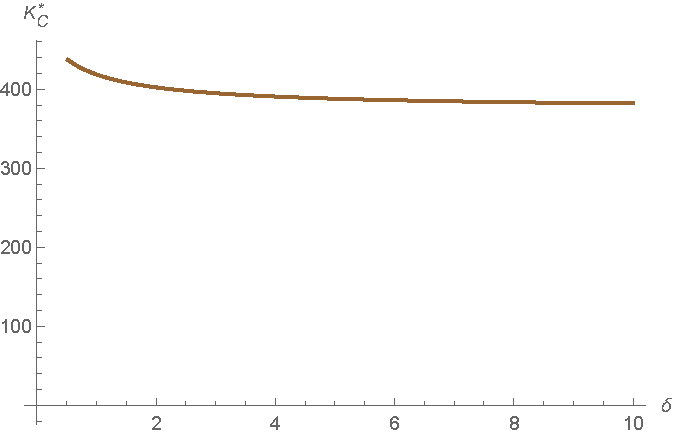
\includegraphics[width=0.45\textwidth]{Prob2_CapOpt/koptx_delta.pdf}}
	\end{subfigmatrix}
	\caption{Optimal capacity regarding the threshold value $x^*_C$.}
	\label{fig:2_k3}
\end{figure}

Regarding discount rate $r$ and sensibility parameter $\alpha$, we have on Figure \ref{fig:2_k2} that $K^*_C$ decreases with them, as happened in the previous section.

\begin{figure}[!htb]
	\begin{subfigmatrix}{2}
		\subfigure[$ r \in ( \mu, 1 )$]{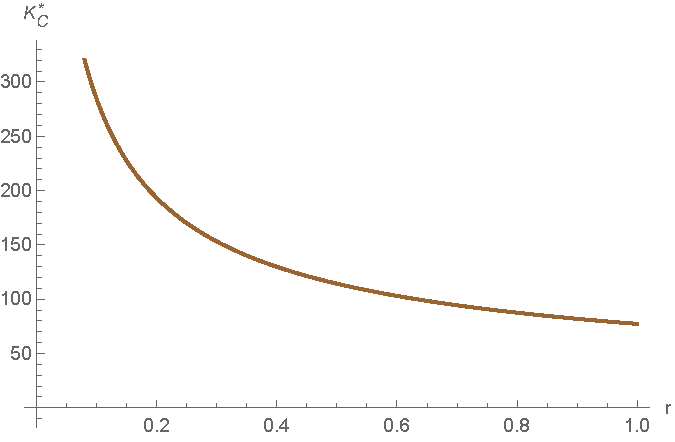
\includegraphics[width=0.45\textwidth]{Prob2_CapOpt/koptx_r.pdf}}
		\subfigure[$ \alpha \in (0,1)$]{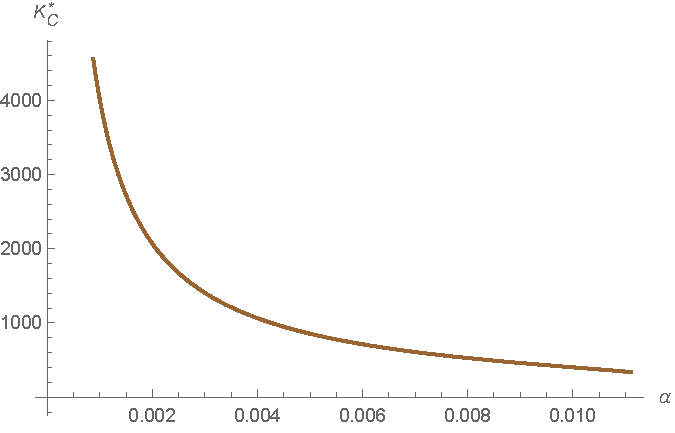
\includegraphics[width=0.45\textwidth]{Prob2_CapOpt/koptx_alpha.pdf}}
	\end{subfigmatrix}
	\caption{Optimal capacity regarding the threshold value $x^*_C$.}
	\label{fig:2_k2}
\end{figure} % file "Thesis_Implementation.tex"
\cleardoublepage

%\input{Thesis_new_file} % add new .tex files for new chapters
% \cleardoublepage

%\input{Thesis_new_file} % add new .tex files for new chapters
% \cleardoublepage

%\input{Thesis_new_file} % add new .tex files for new chapters
% \cleardoublepage
%%%%%%%%%%%%%%%%%%%%%%%%%%%%%%%%%%%%%%%%%%%%%%%%%%%%%%%%%%%%%%%%%%%%%%%%
%                                                                      %
%     File: Thesis_Results.tex                                         %
%     Tex Master: Thesis.tex                                           %
%                                                                      %
%     Author: Andre C. Marta                                           %
%     Last modified :  2 Jul 2015                                      %
%                                                                      %
%%%%%%%%%%%%%%%%%%%%%%%%%%%%%%%%%%%%%%%%%%%%%%%%%%%%%%%%%%%%%%%%%%%%%%%%

\chapter{Investing in a new product with cannibalisation when the firm is already active}
\label{chapter:3}


%Insert your chapter material here...

%%%%%%%%%%%%%%%%%%%%%%%%%%%%%%%%%%%%%%%%%%%%%%%%%%%%%%%%%%%%%%%%%%%%%%%%
\section{Introduction}
\label{section:3_intro}

%We increase the complexity of our problem by considering that the firm has three different states of production.

%In the first state, we consider that the firm only produces a (very) \textit{stable} product, that does not depend on the demand observe. We will call it \textit{old} product. Its demand function $p_0$ and instaneous profit function $\pi_0$ are the same as stated in Chapter \ref{chapter:2} and take the values of \eqref{p0} and \eqref{pi0}, respectively.

%In the second state, we consider the firm produces simultaneously the \textit{old} product and a new one. We will call it \textit{new} product. This \textit{new} product is inserted in the market since after the innovation process as achieved a certain innovation level, \textit{a priori} defined. Since it's based on a new technology and it's a product that is not know by people, we will consider that its profit depends on the demand level.

We extend the situation described on the previous chapter by considering a firm, which has an established product in the market, and wants to find the best time to:
\begin{enumerate}
	\item Invest and introduce in the market an innovative product with technology level $\theta$, allowing the possibility of a simultaneous production of both \textit{old} and \textit{new} products;
	\item Abandon the production of the \textit{old} product, maintaining the \textit{new} one in the market.
\end{enumerate}

Consequently, as showed on Figure \ref{3_time}, the firm faces 3 stages.

\vspace{4mm}
\begin{figure}[!htb]
	\centering
	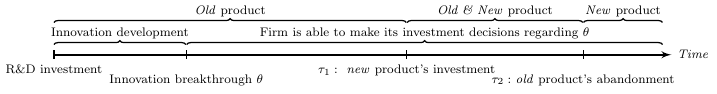
\includegraphics[width=\textwidth]{Prob3/3_timelinet.PNG}
	\caption{Timeline representing the three possible different stages of production and associated decisions. In this chapter time is set to start at the innovation breakthrough.}
	\label{3_time}
\end{figure}
On the first one only the established\&old product is produced, whose unitary price $p_0$ and profit functions $\pi_0$ are the same as stated in Chapter \ref{chapter:2} and take the values of \eqref{p0} and \eqref{pi0}, respectively.

During the second stage the firm produces both \textit{old} and \textit{new} products, leading to the follow profit functions
\begin{align}
\pi_0^A(X_t)&=(1-\alpha K_0-\eta K_1 X_t) K_0\\
\pi_1^A(X_t)&=(\theta-\alpha K_1-\eta K_0 X_t) K_1.
\end{align}

A \textit{cannibalisation} (or\textit{ horizontal differentiation}) parameter $\eta$ is introduced on both expressions to embody the crossed effect between the \textit{old} and the \textit{new} product. As we consider both products to be interacting in the same market, $\eta$ represents the penalty that the quantity
associated to a product will influence the price of the other. We consider here
that this influence is the same for both products, so we can have a unique cannibalisation parameter $\eta$.
By observing that $\eta\geq \alpha$ would imply a larger effect on the product price that on the quantity of production itself, we establish $\eta$ to be such that $\eta < \alpha$. 
By adding both profits $\pi^A_0$ and $\pi_1^A$ we attain the profit associated to this second stage, that is,
%Therefore the resultant profit function associated to this second state of production is denoted by $\pi_A$ and it is such that
\begin{equation}
\pi_A(X_t)=\pi_0^A(X_t)+\pi_1^A(X_t)=(1-\alpha K_0)K_0+(\theta-\alpha K_1)K_1X_t-2\eta K_0 K_1 X_t.
\end{equation}
%\begin{align}
%\pi_0^A(X_t)&=(1-\alpha K_0-\eta K_1 X_t) K_0\\
%\pi_1^A(X_t)&=(\theta-\alpha K_1-\eta K_0 X_t) K_1.
%\end{align}

%However this one cannot be greater than the sensibility parameter $\alpha$ ($\eta<\alpha$). Otherwise, the quantity of the other product would have a larger effect on the product price than the quantity of the product itself.




%The instantaneous profit functions associated to the \textit{old} and the \textit{new} product, during the simultaneous production, are given respectively by
%\begin{align}
%\pi_0^A(X_t)&=(1-\alpha K_0-\eta K_1 X_t) K_0\\
%\pi_1^A(X_t)&=(\theta-\alpha K_1-\eta K_0 X_t) K_1.
%\end{align}


%We need to consider a \textit{cannibalisation} (or\textit{ horizontal differentiation}) parameter $\eta$ that corresponds to the crossed effect between the \textit{old} and the \textit{new} product. As we consider both products to be interacting in the same market, $\eta$ represents the penalty that the quantity
%associated to a product will influence the price of the other. We consider here
%that this influence is the same for both products, so we can have a unique cannibalisation parameter $\eta$, however this one cannot be greater than the sensibility parameter $\alpha$ ($\eta<\alpha$). Otherwise, the quantity
%of the other product would have a larger effect on the product price than the quantity of the product itself.

%The instantaneous profit function associated to this second state of production is denoted by $\pi_A$ and it is such that
%\begin{equation}
%\pi_A(X_t)=\pi_0^A(X_t)+\pi_1^A(X_t)= \pi_0+\pi_1(X_t)-2\eta K_0 K_1 X_t=(1-\alpha K_0)K_0+(\theta-\alpha K_1)K_1X_t-2\eta K_0 K_1 X_t.
%\end{equation}


Finally, on the third state, we consider that the firm abandons the \textit{old} product and starts producing solely the \textit{new} product, which is not considered to be a stable product. Its demand function $p_1$ and profit function $\pi_1$, as stated in Chapter \ref{chapter:2} and take the values of \eqref{p1} and \eqref{pi1}, respectively.


Therefore we want to find two optimal times to make different (but maybe simultaneous) decisions. We want to find the best time $\tau_1$ to go from the first to the second state - that is, to invest in the \textit{new} product and start producing, simultaneously, the \textit{old} and the \textit{new} product - and we also want to find the best time $\tau_2$ to go from the second to the third state - that is, to replace the production of the \textit{old} product by the \textit{new} one. Note that $\tau_2 \geq \tau_1$ are both stopping times adapted to the natural filtration of the demand process $\{ X_t, \ t\geq0 \}$ and there is no chance on return the production of the \textit{old} product, once the firm had abandoned it in $\tau_2$. Thus these are irreversible choices. 

The strategy followed to calculate $\tau_1$ and $\tau_2$ is the one presented in \cite{dixit:book}. Dixit and Pindyck suggest to firstly
%calculate the value of the project, secondly 
calculate the value of the investment in the second stage and then the value of the investment in the first stage. Although the contexts were different, a similar strategy was used in \cite{rita} - but here having a decision threshold associated with the innovation process, not only the demand as we do - and in \cite{hagspiel:cap} - but considering an entering-or-exit the market situation.

%%%%%%%%%%%%%%%%%%%%%%%%%%%%%%%%%%%%%%%%%%%%%%%%%%%%%%%%%%%%%%%%%%%%%%%%
\section{Stopping Problem}
\label{section:2_theory}



As made in previous sections, we still consider that at the moment we adapt the new product, we need to pay $\delta K_1$ related to sunk costs and that at the precise moment we adapt the new product, we are totally able to produce it. 
%Once again, we set the instant $t=0$ to be the instant immediately after the desired innovation threshold $\theta$ happens.

Taking into account the different profits associated to each state of production, as described on Figure \ref{3_time}, our the optimal stopping problem may be formulated as finding the value function $F$ such that

\begin{align}
F(x)=\sup _{\tau_1} \mathds{E}^{X_0=x} \Bigl[ \int_0^{\tau_1} \pi_0e^{-rs} ds &+ \sup_{\tau_2} \mathds{E}^{X_{\tau_1}=x_{\tau_1}} \Bigl[ \int_{\tau_1}^{\tau_2}  \pi_A(X_s) e^{-rs}ds + \nonumber \\
& +\int_{\tau_2}^\infty \pi_1(X_s)e^{-rs}ds \ \mathds{1}_{ \{\tau_2<\infty \} } -e^{-r \tau_1}\delta K_1  \Bigr] \mathds{1}_{ \{\tau_1<\infty \} } \Bigr]
\label{eq:3_des}
\end{align}


Manipulating \eqref{eq:3_des} by changing the region of integration of the first integral and admitting taht both decisions are made in finite time (with probability 1), we obtain
\begin{align}
F(x)&=\sup _{\tau_1} \mathds{E}^{X_0=x} \Bigl[ \int_0^{\infty} \pi_0e^{-rs} ds +\sup_{\tau_2} \mathds{E}^{X_{\tau_1}=x_{\tau_1}} \Bigl[ \int_{\tau_1}^{\tau_2} \left( \pi_A(X_s)-\pi_0 \right) e^{-rs}ds +  \nonumber \\
&\hspace{4.35cm} +\int_{\tau_1}^\infty \left( \pi_1(X_s)-\pi_0 \right) e^{-rs}ds -e^{-r \tau_1}\delta K_1  \Bigr] \Bigr]   \\
&=\frac{\pi_0}{r}+\sup _{\tau_1} \mathds{E}^{X_0=x} \Bigl[  \sup_{\tau_2} \mathds{E}^{X_{\tau_1}=x_{\tau_1}} \Bigl[ \int_{\tau_1}^{\tau_2} \left( \pi_A(X_s)-\pi_0 \right) e^{-rs}ds + \int_{\tau_2}^\infty \left( \pi_1(X_s)-\pi_0 \right) e^{-rs}ds  \Bigr] -e^{-r \tau_1}\delta K_1 \Bigr] \nonumber
\label{eq:32} 
\end{align}

Changing integration variables of both integrals on the optimization problem related with $\tau_2$ we obtain
\begin{equation}
	\begin{split}
		F(x)=\frac{\pi_0}{r}+\sup _{\tau_1} \mathds{E}^{X_0=x} \Bigl[ e^{-r \tau_1} \Bigl(  \sup_{\tau_2} \mathds{E}^{X_{\tau_1}=x_{\tau_1}} \Bigl[ &\int_0^{\tau_2-\tau_1} \left( \pi_A(X_{\tau_1+s})-\pi_0 \right) e^{-rs}ds +\\
		+&\int_{\tau_2-\tau_1}^\infty \left( \pi_1(X_{\tau_1+s})-\pi_0 \right) e^{-rs}ds  \Bigr]-\delta K_1 \Bigr) \Bigr].
		%\right) \right].
	\end{split}
	\label{eq:3w}
\end{equation}
where since the term $e^{-r \tau_1}$ does not depend on $\tau_2$, it can be put in evidence as made above.


\subsubsection{$\tau_2 \ - $ Optimal Stopping Problem:}

Considering $F_2$ to be the value function associated to the optimal stopping problem related to $\tau_2$ we have that its expression is given by
\begin{equation}
F_2(x)=\sup_{\tau_2} \mathds{E}^{X_{\tau_1}=x_{\tau_1}} \left[ \int_0^{\tau_2-\tau_1} \left( \pi_A(X_{\tau_1+s})-\pi_0 \right) e^{-rs}ds + \int_{\tau_2-\tau_1}^\infty \left( \pi_1(X_{\tau_1+s})-\pi_0 \right) e^{-rs}ds  \right],
\label{eq:34}
\end{equation}
from which follows that our optimal stopping problem, initially given by \eqref{eq:31}, is now given by
\begin{equation}
F(x)=\frac{\pi_0}{r}+\sup _{\tau_1} \mathds{E}^{X_0=x} \left[ e^{-r \tau_1}(F_2(X_{\tau_1})-\delta K_1 )\right].
\label{eq:35}
\end{equation}

In view of $F$, we have two different optimal stopping problems in hands regarding $\tau_1$ and $\tau_2$. We start solving the one concerning the \textit{latest} stopping time, assuming that we know what happened until the
%We have two different optimal stopping problems that we should solve starting on the \textit{latest} stopping time, $\tau_2$, by considering that we know what happened until the 
instant that the firm invests, $\tau_1$. In order to do that, let $\{Y_t, \ t\geq0\}$ be the stochastic process that represents the demand level after occuring the investment at $\tau_1$ and which evolves stochastically accordingly to a GBM with the same drift $\mu$ and volatility $\sigma$ as $\{X_t, \ t\geq0\}$, that is $\{Y_t, \ t\geq0\} = \{X_{\tau_1+t}, \ t\geq0\}$. Note that it's initial value is the same as observed at the instant $\tau_1$, that is $Y_0=X_{\tau_1}$.

Consider as well $\tau$ to be the stopping time, adapted to the natural filtration of the process $\{Y_t, \ t\geq0\}$. Observe that $\tau$ represents the optimal time for which the firm should make the replacement of the \textit{old} product by the \textit{new} one, after having invested at time $\tau_1$. This means that  if $\tau=0$, then the old product is replaced by the new one at the precise instant when the investment happens $\tau_1$. Note that $\tau$ is also adapted to the natural filtration of $\{ X_{\tau+t},\ t\geq0 \}$ and that $\tau_2=\tau_1+\tau$. Thus, by knowing $\tau_1$ and finding $\tau$, we can calculate $\tau_2$.

Therefore, $F_2$, as written in \eqref{eq:34}, is equivalent to
\begin{equation}
F_2(x_{\tau_1})=\sup_{\tau} \mathds{E}^{Y_0=x_{\tau_1}} \left[ \int_0^{\tau} \left( \pi_A(Y_s)-\pi_0 \right) e^{-rs}ds + \int_{\tau}^\infty \left( \pi_1(Y_s)-\pi_0 \right) e^{-rs}ds  \right],
\label{eq:3s2}
\end{equation}
%In case we want to calculate $\tau_2$, we just need to add the stopping times $\tau_1$ and $\tau$.
meaning that, in accordance to Figure \ref{3_time}, from time 0 to time $\tau$, the firm is producing both products and that, from time $\tau$ on, the firm only produces the \textit{new} product, where the instant 0 corresponds to the instant when the firm decides to invest, $\tau_1$.

Fortunately we can simplify the notation of \eqref{eq:3s2}. Since the Strong Markov property states that after a stopping time, the future path of the GBM depends only on the value at the stopping time (knowing this one), it follows that 
$$\{(Y_t | Y_0=x_{\tau_1}), \ t\geq0 \} = \{(X_{\tau_1+t} | X_{\tau_1}=x_{\tau_1}),\ t\geq \tau_1 \} \overset{d}{=}  \{(X_{t}, | X_0=x_{\tau_1}), \ t\geq0 \}. $$

Therefore we can keep the same notation as before and thus from \eqref{eq:3s2} follows
\begin{equation}
F_2(x_{\tau_1})=\sup_{\tau} \mathds{E}^{X_0=x_{\tau_1}} \left[ \int_0^{\tau} \left( \pi_A(X_s)-\pi_0 \right) e^{-rs}ds + \int_{\tau}^\infty \left( \pi_1(X_s)-\pi_0 \right) e^{-rs}ds  \right].
\label{eq:3s3}
\end{equation}

%We haven't forgotten the term $e^{-r \tau_1}$. However since it's irrelevant for the current optimization problem, we will only proceed with it when writing the full problem. 

Using the fact that the expectation is a linear operator, we treat the expectation of the rightmost integral of \eqref{eq:3s3} separately, that is
\begin{equation}
\mathds{E}^{X_0=x_{\tau_1}} \left[  \int_{\tau}^\infty \left( \pi_1(X_s)-\pi_0 \right) e^{-rs}ds  \right] =  e^{-r\tau} \mathds{E}^{X_0=x_{\tau_1}} \left[  \int_{0}^\infty \left( \pi_1(X_{\tau+s})-\pi_0 \right) e^{-rs}ds  \right].
\label{eq:3s4}
\end{equation}

Conditioning to the stopping time $\tau$ and using Tower Rule we obtain from \eqref{eq:3s4}
\begin{equation}
e^{-r\tau} \mathds{E}^{X_0=x_{\tau_1}} \left[ \mathds{E}^{\tau}  \left[ \int_{0}^\infty \left( \pi_1(X_{t+s})-\pi_0 \right) e^{-rs}ds  \right] \right].
\label{eq:3s5}
\end{equation}

Using the similar arguments as in Section \ref{subsec:1_bm}, we interchange the integral with expectation using Fubini's theorem and the fact that $r-\mu>0$, obtaining
\begin{equation}
e^{-r\tau} \mathds{E}^{X_0=x_{\tau_1}} \left[  \int_{0}^\infty \mathds{E}^{\tau}  \left[ \pi_1(X_{t+s}) e^{-rs}  \right] ds - \frac{\pi_0}{r} \right]=  e^{-r\tau} \mathds{E}^{X_0=x_{\tau_1}} \left[    (\theta-\alpha K_1)K_1  \int_{0}^\infty \mathds{E}^{\tau}  \left[  X_{t+s} e^{-rs}  \right] ds - \frac{\pi_0}{r} \right],
\label{eq:3s6}
\end{equation}
where the term $ (\theta-\alpha K_1)K_1$ is constant over time.

%Since $\tau$ is a stopping time and that by knowing its value, we also know the observed value of GBM at time $\tau$, by the Strong Markov property it follows from \eqref{eq:3s6} 


We focus now on the expected value conditional to the stopping time $\tau$ above. 
Since the demand level evolves accordingly to a GBM, it follows 
%and, by knowing the instant $\tau$, we know its value at time $\tau$ - here denoted as $x_\tau$ -, it follows 
\begin{align}
\mathds{E}^{\tau}  \left[  X_{\tau+s}e^{-rs}  \right] 
&=\mathds{E}^{\tau}  \left[  X_{\tau} e^{\left( \mu- \frac{\sigma^2}{2}-r \right)   (\tau+s-\tau)+\sigma( W_{\tau+s}-W_\tau)}  \right]  \nonumber \\
&=\mathds{E}^{\tau}  \left[  X_{\tau} e^{\left( \mu- \frac{\sigma^2}{2}-r \right) s+\sigma W_{s}}   \right]  \nonumber \\
&= X_{\tau} e^{\left( \mu-r \right)s},
\label{eq:3s8}
\end{align}
where in the second equality we used the fact that Brownian Motion $\{ W_t, \ t \geq0 \}$ has stationary increments, that is 
$$W_{\tau+s}-W_\tau \overset{d}{=} W_{\tau+s-\tau}-W_0 \overset{d}{=} W_{s} \sim \mathcal{N}(0,s).$$



%Interchanging the integral with expectation using Fubini's theorem and the fact that $r-\mu>0$ we obtain
%\begin{equation}
%  e^{-r\tau} \mathds{E}^{X_0=x_{\tau_1}} \left[  \int_{0}^\infty \mathds{E}^{\tau=t}  \left[  \pi_1(X_{t})e^{-rs}  \right] ds -\frac{\pi_0}{r} \right]=e^{-r\tau} \mathds{E}^{X_0=x_{\tau_1}} \left[   (\theta-\alpha K_1)K_1 \int_{0}^\infty \mathds{E}^{\tau=t}  \left[  X_{t}e^{-rs}  \right] ds -\frac{\pi_0}{r} \right],
%    \label{eq:3s6}
%\end{equation}
%where the term $ (\theta-\alpha K_1)K_1$ is constant over time.

%We focus now in the expected value above. Recall that the demand level evolves accordingly with a GBM and thus
%\begin{align}
%    \mathds{E}^{\tau=t}  \left[  X_{t}e^{-rs}  \right] &=\mathds{E}^{\tau=t}  \left[  x_{\tau_1} e^{\left( \mu- \frac{\sigma^2}{2}-r \right)   (\tau+s-\tau)+\sigma( W_{\tau+s}-W_\tau)}  \right]\\
%    &=\mathds{E}^{\tau=t}  \left[  x_{\tau_1} e^{\left( \mu- \frac{\sigma^2}{2}-r \right) s+\sigma W_{s}}   \right] \\
%    &= x_{\tau_1} e^{\left( \mu-r \right)s},
%    \label{eq:3s7}
%\end{align}
%where in the second equality we used the fact that Brownian Motion has stationary increments, that is 
%$$W_{\tau+s}-W_\tau =^d W_{\tau+s-\tau}-W_0 =^d W_{s} \sim \mathcal{N}(0,s).$$
Plugging \eqref{eq:3s8} in \eqref{eq:3s6}, we obtain
\begin{equation}
e^{-r\tau} \mathds{E}^{X_0=x_{\tau_1}} \left[   (\theta-\alpha K_1)K_1 \int_{0}^\infty x_{\tau_1} e^{\left( \mu-r \right)s} ds -\frac{\pi_0}{r} \right] = e^{-r\tau} \mathds{E}^{X_0=x_{\tau_1}} \left[   \frac{(\theta-\alpha K_1)K_1}{r-\mu} x_{\tau} -\frac{\pi_0}{r} \right].
\label{eq:3s9}
\end{equation}

Therefore we have found the terminal function associated to the optimal stopping problem $F_2$. Denoting it by $h_2$, it's given by
$$h_2(x)=\frac{(\theta-\alpha K_1)K_1}{r-\mu} x -\frac{\pi_0}{r}.$$

Accordingly to \eqref{eq:3s3}, we may also denote $g_2$ as the running cost function associated to this problem, that is given by
$$g_2(x)=\pi_A(x)-\pi_0.$$

Thus, plugging expression of running and terminal functions on \eqref{eq:3s3}, we have that $F_2$ as initially written in \eqref{eq:34}, is equivalent to
\begin{align}
F_2(x)&=\sup_{\tau} \mathds{E}^{X_0=x} \left[ \int_0^{\tau} g(X_s) e^{-rs}ds + e^{-r\tau}h(X_\tau)  \right]\\
&=\sup_{\tau} \mathds{E}^{X_0=x} \left[ \int_0^{\tau} \left( \pi_0^A(X_s)+\pi_1^A(X_s)-\pi_0 \right) e^{-rs}ds + e^{-r\tau} \left(   \frac{(\theta-\alpha K_1)K_1}{r-\mu} X_{\tau} -\frac{\pi_0}{r} \right)  \right],
\label{eq:3s10}
\end{align}
being this a standard optimal stopping problem.

Since the HJB variational inequality associated to \eqref{eq:3s10}, implies that the non-homogeneous PDE 
\begin{equation}
\frac{\sigma^2}{2}x^2F_2''(x)+\mu x F_2'(x) - r F_2(x)+g(x) =0 
\label{3hjb}
\end{equation}
holds for any demand value in the continuation region, it follows that its solution $F_2$ takes the form of
\begin{equation}
F_2(x)=F_{2,h}(x)+F_{2,p} \quad \forall x \in \mathcal{C},
\end{equation}
where $F_{2,h}$ corresponds to the solution to the homogeneous version of the PDE in \eqref{3hjb}, $F_{2,p}$ to a particular solution of \eqref{3hjb} and $\mathcal{C}$ to the continuation region of the form $\{ x \in \mathds{R}: x< x_2^* \}$.

We first calculate the particular solution $F_{2,p}$. By considering $F''_{2,p}(x)=0$ and using expression \eqref{3hjb}, a particular solution is found to be 
\begin{equation}
F_{2,p}(x)=\frac{(\theta-\alpha K_1)K_1-2 \eta K_0 K_1}{r-\mu}x \  \   \xrightarrow[x \rightarrow 0 ]{ } \ 0
	\label{F2p}
\end{equation}

% Note that $\underset{x \to 0}{\text{lim}} F_{2,p}(x)=0$. This fact is an useful detail when it comes to calculate $F_2$.

Since there is no possibility of having a project having a negative value it follows $F_2(x) \geq 0 \ \forall x \in \mathcal{C}$. From \ref{F2p}, we obtain that $F_{2,h}=a_2 x^{d_1}+b_2 x^{d_2}$ simplifies to $F_{2,h}=a_2 x^{d_1}$ guaranteeing this way that $\underset{x \to 0}{\text{lim}} F_2(x)=\underset{x \to 0}{\text{lim}} F_{2,h}(x)+F_{2,p}(x)=0$.

Once again, the constant term $a_2$ and the demand level that triggers the abandonment of the \textit{old} product $x_2^*$ are found by value matching \eqref{valuematch} and smooth pasting \eqref{smoothpasting} conditions, expressed by
\begin{equation}
\begin{cases}
a_2(x_2^*)^{d_1}+\frac{(\theta-\alpha K_1)K_1-2 \eta K_0 K_1}{r-\mu}x_2^*=\frac{(\theta-\alpha K_1)K_1}{r-\mu} x_2^* -\frac{\pi_0}{r} \\
a_2 d_1(x_2^*)^{d_1-1}+\frac{(\theta-\alpha K_1)K_1-2 \eta K_0 K_1}{r-\mu}=\frac{(\theta-\alpha K_1)K_1}{r-\mu}
\end{cases},
\end{equation}
from which we obtain
\begin{align}
a_2 &= \left( \frac{2\eta K_0 K_1}{r-\mu}x^*-\frac{\pi_0}{r} \right)(x_2^*)^{-d_1} \nonumber \\
x_2^*&=\frac{d_1}{d_1-1} \frac{1-\alpha K_0}{2 \eta K_1} \frac{r-\mu}{r} \label{3:x2}
\end{align}
%Taking into account that the instantaneous profit associated to the time when both (\textit{old} and \textit{new}) products are being produced cannot be negative, that is $\pi_A(X_t) \geq 0 \ \forall t \geq 0$, we obtain that $F_2 \geq 0$ 

Taking into account that $F_2$ is also defined in the stopping region, we obtain that its expression is given by
\begin{equation}
F_2(x)=\left( a_2 x^{d_1} +\frac{(\theta-\alpha K_1)K_1-2 \eta K_0 K_1}{r-\mu}x \right) \mathds{1}_{ \{ x<x_2^* \} }+ \left( \frac{(\theta-\alpha K_1)K_1}{r-\mu} x -\frac{\pi_0}{r} \right)\mathds{1}_{ \{ x\geq x_2^* \} },
\label{eq:f2}
\end{equation}

\subsubsection{$\tau_1 \ - $ Optimal Stopping Problem:}

We are now in position to return to the main problem, as lastly described in \eqref{eq:35}. Re-evaluating with the expression deduced for $F_2$, it takes the form of
\begin{equation}
F(x)=\frac{\pi_0}{r}+\sup _{\tau_1} \mathds{E}^{X_0=x} \left[ e^{-r \tau_1} \left( \frac{(\theta-\alpha K_1)K_1}{r-\mu} X_{\tau_1}+ 
\left( a X_{\tau_1}^{d_1} -\frac{2 \eta K_0 K_1}{r-\mu} X_{\tau_1} \right) \mathds{1}_{ \{X_{\tau_1}<x_2^* \} } -\frac{\pi_0}{r}\mathds{1}_{ \{ X_{\tau_1} \geq x_2^* \} }
-\delta K_1 \right) \right],
\label{eq:f2x}
\end{equation}
which isagain an optimal problem with null running cost function, however this time with two terminal cost functions defined on disjoint domains. Thereat, we obtain two optimal times associated to the adoption of the innovative product, depending on whether we allow a simultaneous production period or not. These are depending on the following demand thresholds: 

%We still want to find the optimal time $\tau_1$ to make the investment decision. However as the problem is stated in \eqref{eq:f2x}, we obtain two different demand threshold levels:
\begin{itemize}
	\item $x_{1,A}^*$:
	this is the threshold that triggers the investment and the addition of the \textit{new} product to the market, starting a period of simultaneous production. Therefore it is associated to the region $X_{\tau_1} < x^*_2$ so as to the following stopping problem %we add the \textit{new} product and have a period of simultaneously production. It is associated to the region $$ and to the stopping problem
	\begin{equation}
	%\underset{\tau_1}{\text{sup}} 
	\sup_{\tau_1} \mathds{E}^{X_0=x} \left[ e^{-r \tau_1} \left( \frac{(\theta-\alpha K_1)K_1-2 \eta K_0 K_1}{r-\mu} X_{\tau_1}+
	 a_2 X_{\tau_1}^{d_1} - \delta K_1 \right) \right],
	 \label{3:add}
	 \end{equation}
	 where the decision is made on finite time $\tau$ with probability 1. Note that when the demand observes larger values than $x^*_2$ its respective value is given by the expression on the rightmost side of \eqref{eq:f2x}.
	\item $x_{1,R}^*$: this is the threshold associated to the region $X_{\tau_1} \geq x^*_2$ for which the firm invest in the new product by immediately replacing the one established in the market. Considering that the investment decision is made in finite time with probability 1, this situation leads to the following stopping problem
	%we add the \textit{new} product and immediately replace the old one. It is associated to the region $X_{\tau_1} \geq x^*_2$ and to the stopping problem
	\begin{equation}
	%\underset{\tau_1}{\text{sup}} 
	\sup_{\tau_1} \mathds{E}^{X_0=x} \left[ e^{-r \tau_1} \left( \frac{(\theta-\alpha K_1)K_1}{r-\mu} X_{\tau_1}-
	\frac{\pi_0}{r} - \delta K_1 \right) \right]
	\label{3:r}
	\end{equation}
\end{itemize}

We will deduce both thresholds $x_{1,A}^*$ and $x_{1,R}^*$ by its respective order.
\\
\textbf{$\bullet$ Demand threshold $x^*_{1,A}$:}

The optimal stopping problem stated in \eqref{3:add} is a standard optimal stopping problem, for which we don't have a solution (yet).
Denoting by $F_{1,A}$ its correspondent solution we have that $F_{1,A}$ verifies the HJB variational inequality \eqref{HJB}, where we take the terminal function to be $h(x)=\frac{(\theta-\alpha K_1)K_1-2 \eta K_0 K_1}{r-\mu} X_{\tau_1}+
a_2 X_{\tau_1}^{d_1} - \delta K_1$. Therefore it follows that $F_{1,A}$ takes the form
\begin{equation}
F_{1,A}(x)=\begin{cases} a_{1,A} x^{d_1}  &\ , \ x \in \mathcal{C}_{1,A} \\
\frac{(\theta-\alpha K_1)K_1-2 \eta K_0 K_1}{r-\mu} x+
a_2 x^{d_1} - \delta K_1 &\ , \ x \in \mathcal{S}_{1,A}
\end{cases},
\label{3_F1A}
\end{equation}
with $\mathcal{C}_{1,A}$ here considered to be the continuation region of the form $\{ x \in \mathds{R}: x<x^*_{1,A} \}$. The threshold value $x_{1,A}^*$ and coefficient $a_{1,A}$ are found by value matching \eqref{valuematch} and smooth pasting \eqref{smoothpasting} conditions, expressed by the corresponding system
\begin{equation}
\begin{cases} a_{1,A} (x_{1,A}^*)^{d_1}=\frac{(\theta-\alpha K_1)K_1-2 \eta K_0 K_1}{r-\mu} x_{1,A}^*+
a_2 (x_{1,A}^*)^{d_1} - \delta K_1\\
a_{1,A} d_1(x_{1,A}^*)^{d_1-1}=\frac{(\theta-\alpha K_1)K_1-2 \eta K_0 K_1}{r-\mu}+
a_2 d_1 (x_{1,A}^*)^{d_1-1}
\end{cases},
\label{eq:3_sistema}
\end{equation}
from which we obtain
\begin{align}
x_{1,A}^*&=\frac{d_1}{d_1-1} \frac{\delta K_1 (r-\mu )}{ (\theta -\alpha  K_1)K_1-2 \eta  K_0 K_1} \label{eq:3_x1A}\\
a_{1,A}&=
a_2 x^*_2+\frac{((\theta -\alpha  K_1)K_1-2 \eta  K_1 K_0) }{r-\mu }(x_{1,A}^*)^{1-d_1}-\delta K_1 (x_{1,A}^*)^{-d_1}.
\label{3:a1A} 
%&= \frac{2^{\text{dd1}} \eta  k \text{k0} \left(\frac{\text{dd1} (1-\alpha  \text{k0}) (r-\mu )}{(\text{dd1}-1) \eta  k r}\right)^{1-\text{dd1}}}{\text{dd1} (r-\mu )}
\end{align}
%with $d_1$ being the positive root of the polynomial described in \eqref{d1}.

Observe that since the threshold $x_{1,A}^*$ needs always to be positive, the following restriction must hold
\begin{equation}
	(\theta -\alpha  K_1)K_1-2 \eta  K_0 K_1>0 \ \Leftrightarrow \ K_1 < \frac{\theta}{\alpha + 2\eta K_0} \leq \frac{\theta}{\alpha},
	\label{3_cond}
\end{equation}
where the equality (in the last inequality) holds for $\eta=0$. 

Thus the solution associated to $\eqref{3:add}$ is given by 
\begin{equation}
F_{1,A}(x)= \left(  a_{1,A}x^{d_1} \mathds{1}_{ \{ x<x^*_{1,A}\}} +
\left(  \frac{(\theta-\alpha K_1)K_1-2 \eta K_0 K_1}{r-\mu} x+
a_2 x^{d_1} - \delta K_1 \right)  \mathds{1}_{ \{ x \geq x^*_{1,A} \}} \right)  \mathds{1}_{ \{   x < x_2^*  \}},
\label{3:Fadd}
\end{equation}
continuation and stopping regions are respectively described as in \eqref{c_region} and \eqref{s_region} and the optimal stopping time as in \eqref{stoptime}.


\textbf{$\bullet$ Demand threshold $x^*_{1,R}$:}

Note that the optimal stopping problem \eqref{3:r} is the same as the one explored and analysed in Chapter \ref{chapter:2}, consisting in the benchmark model (Section \ref{2_bm}).
Thus it follows that the threshold level is given by \eqref{2_xB}, that is,
\begin{equation}
x^*_{1,R}=\frac{d_1}{d_1-1} \frac{ \delta K_1  +\frac{\pi_0}{r} }{\theta-\alpha K_1} \frac{r-\mu}{K_1}.
\label{3_x1R}
\end{equation}
On the other side the solution associated to $\eqref{3:r}$ is given by \eqref{2:Fbm}, that is, (changing the name of the associated solution)
\begin{equation}
F_{1,R}(x)= \left(  a_{1,R}x^{d_1} \mathds{1}_{ \{ x<x^*_{1,R}\}} +
\left(  \frac{(\theta-\alpha K_1)K_1 x}{r-\mu} - \delta K_1  -\frac{\pi_0}{r}\right)  \mathds{1}_{ \{ x \geq x^*_{1,R}\}} \right) \mathds{1}_{ \{ x \geq x^*_2\}} ,
\label{3:Fr}
\end{equation}
with $a_{1,R}$ taking the same value as $a_2$ in \eqref{2_aB}.


Note that from \eqref{3:Fadd} it is impossible to observe a demand threshold $x_2^*$ smaller than $x_{1,A}^*$. This would mean that at the precise instant $x_{1,A}^*$ was reached, we should immediately replace the \textit{old} product by the \textit{new} one. However, this case is not related with thresholds $x_{1,A}$ or $x_2^*$, but with $x_{1,R}^*$.
Therefore we are able to constraint the domains of both functions $F_{1,A}$ and $F_{1,R}$ by analysing under which conditions $x_{1,A}^*<x^*_2$ holds:
\begin{align}
x_{1,A}^*<x_2^* \ &\Leftrightarrow \ \frac{d_1}{d_1-1} \frac{1-\alpha K_0}{2 \eta K_1} \frac{r-\mu}{r} = \frac{d_1}{d_1-1} \frac{\delta K_1 (r-\mu)}{(\theta-\alpha K_1)K_1-2\eta K_0 K_1} \nonumber \\
&\Leftrightarrow \ (1-\alpha K_0) ((\theta-\alpha K_1)K_1-2\eta K_0 K_1)=2 \eta \delta K_1^2 r 
 \nonumber \\
&\Leftrightarrow \ \eta <\frac{(1-\alpha K_0)(\theta-\alpha K_1)}{2(\delta K_1 r + \pi_0)}=: \eta^*, \label{3_eta*}
\end{align}
where we denoted $\eta^*$ to be the cannibalization threshold that states which value function stands.

Therefore we obtain that our problem, as stated in \eqref{eq:f2x}, may be written as

\begin{equation}
F(x)=\frac{\pi_0}{r} + \begin{cases}
a_{1,A}x^{d_1}  &, \ x<x_{1,A} \  \wedge \ \eta<\eta^*\\
a_2x^{d_1}+\frac{(\theta-\alpha K_1)K_1-2 \eta K_0 K_1}{r-\mu} x - \delta K_1 &, \ x_{1,A} \leq x < x_2^* \ \wedge \ \eta<\eta^*\\
a_{1,R}x^{d_1} &, \ x<x_{1,R}^*  \ \wedge \ \eta\geq \eta^* \\
\frac{(\theta-\alpha K_1)K_1 x}{r-\mu} -\frac{\pi_0}{r} - \delta K_1   &, \ ( x>x_2^* \ \wedge \ \eta<\eta^*) \ \overset{.}{\vee} \ (x>x_{1,R}^* \ \wedge \ \eta \geq \eta^*) \\
\end{cases}
	\label{3_madzbigboy}
\end{equation}
with $a_{1,A}$ as described in \eqref{3:a1A}, $a_{1,R}$ as described in \eqref{2_aB}, $x^*_{1,A}$ as described in \eqref{eq:3_x1A}, $x^*_{1,R}$ as described in \eqref{2_xB}, $x^*_2$ as described in \eqref{3:x2} and $\eta^*$ as described in \eqref{3_eta*} (and $\pi_0$ as described in \eqref{pi0}).


\section{Comparative Statics}

%Before we start to analyse how parameters influence the three different threshold levels, we will show how one should interpret the results obtained in \eqref{3_madzbigboy}.

On this chapter, for a better understanding of numerical experiments' results, we consider different values from the ones stated so far. These are given by:
\begin{table*}[!htb]
	\centering
	\begin{tabular}{lllllll}
		$\bullet$ & $\mu=0.45$     &  & \hspace{7cm} &  &  $\bullet$ & $\alpha=0.015$ \\
		$\bullet$ & $\sigma=0.6$ &  & \hspace{7cm} &  &  $\bullet$ & $\theta=1.5$   \\
		$\bullet$ & $r=0.85$       &  & \hspace{7cm} &  &  $\bullet$ & $K_0=51.5$       \\
		$\bullet$ & $\delta=0.95$     &  & \hspace{7cm} & &  $\bullet$ & $K_1=2.5$                              
	\end{tabular}
\end{table*}

On Figure \ref{fig:3_F} we assess the cannibalization threshold $\eta^*$ and how value functions relate to it. In each column we can find a different $\eta$ tested. On the first row we plot all subfunctions possible (respecting the order as they appear in \eqref{3_madzbigboy}) and associated to the value function $F$, without considering the constant term $\frac{\pi_0}{r}$. The final version of it is represented on the first row.
%and playing with the cannibalization parameter $\eta$, we obtain the six plots represented on Figure \ref{fig:3_F}.

%Each column corresponds a different value of $\eta$ set. In each plot of the first row it's represented the different possible parts associated to the value function $F$ \eqref{3_madzbigboy}, accordingly to the respective legend, being the red dashed line corresponding to the valid value function associated to the parameters considered. It is also represented the three possible thresholds: $x_{1,A}^*$ by the yellow dot, $x^*_2$ by the orange dot and $x_{1,R}^*$ by the black dot. Finally on the second row it's represented solely the value function $F$ associated (the same as showed in the respective plot above) and respective threshold values.

\begin{figure}[!htb]
	\begin{subfigmatrix}{6}
		\subfigure[$\eta=0.007$ ]{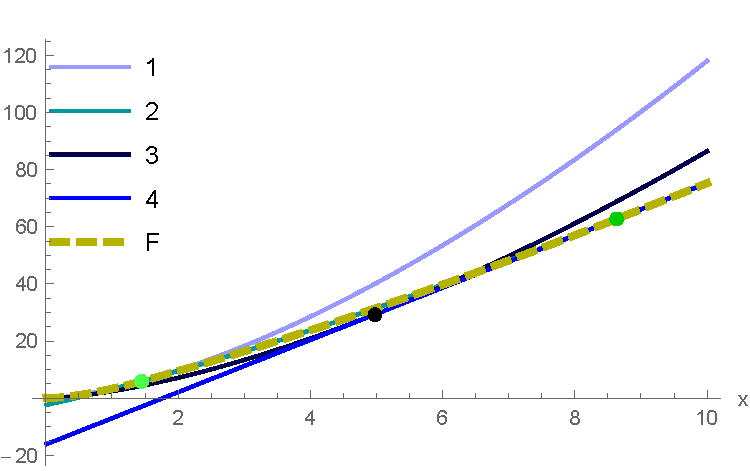
\includegraphics[width=0.32\textwidth]{Prob3/eta007_1.pdf}}
		\subfigure[$\eta=0.012$ ]{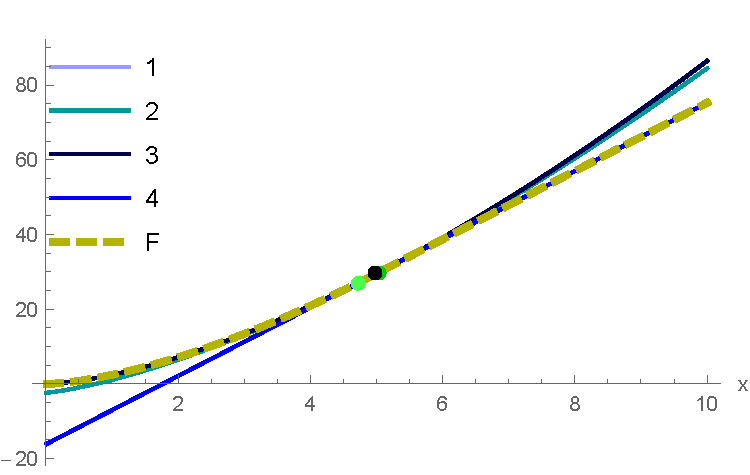
\includegraphics[width=0.32\textwidth]{Prob3/eta0121_1.pdf}}
		\subfigure[$\eta=0.013$ ]{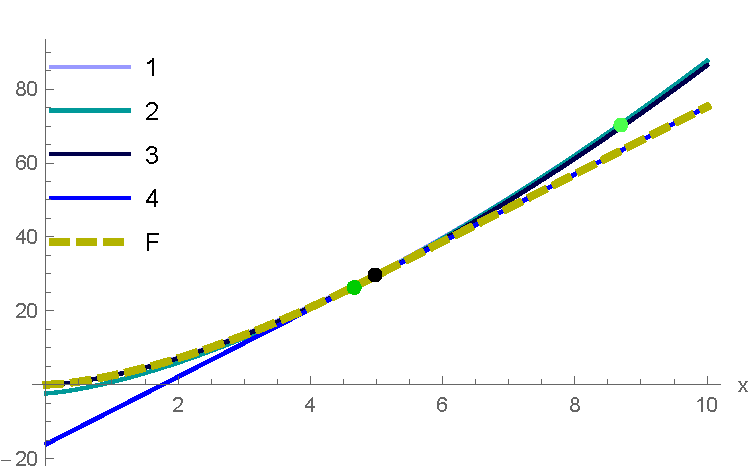
\includegraphics[width=0.32\textwidth]{Prob3/eta013_1.pdf}}
		\subfigure[$\eta=0.007$]{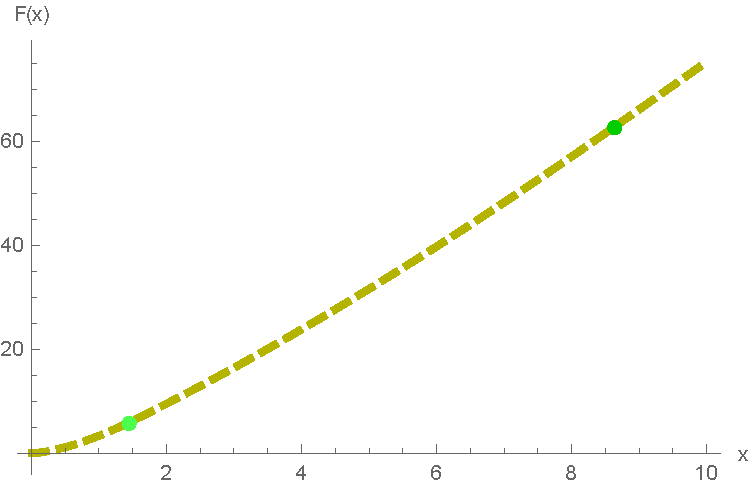
\includegraphics[width=0.32\textwidth]{Prob3/eta007dash_1.pdf}}
		\subfigure[$\eta=0.012$]{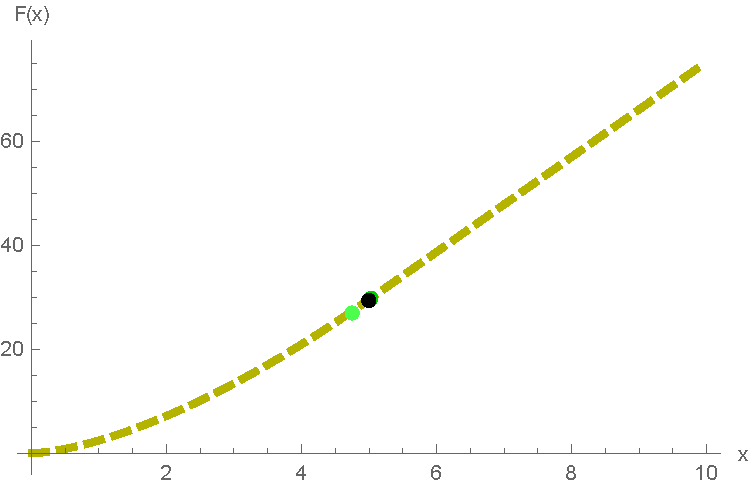
\includegraphics[width=0.32\textwidth]{Prob3/eta012dash_1.pdf}}
		\subfigure[$\eta=0.013$]{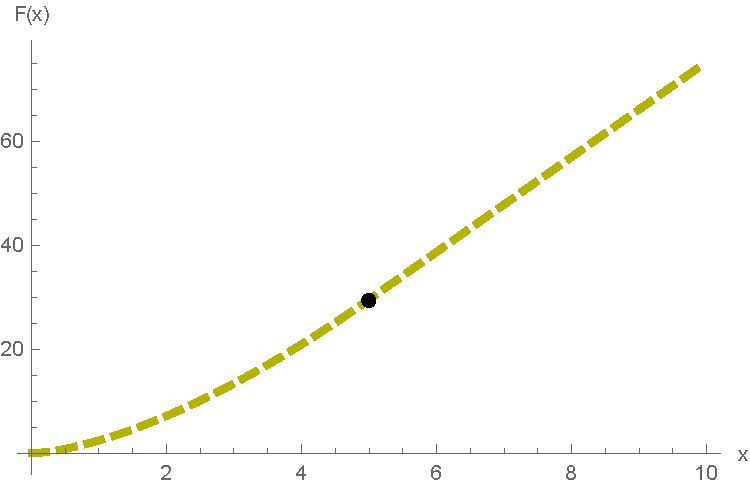
\includegraphics[width=0.32\textwidth]{Prob3/eta013dash.pdf}}
	\end{subfigmatrix}
	\caption{Value function $F$ and respective subfunctions, given the order in \eqref{3_madzbigboy}, associated to different settings of parameter $\eta$.}
	\label{fig:3_F}
\end{figure}

First, note that regarding this set of values, we obtain a cannibalisation threshold $\eta^*\simeq 0.0121$. Therefore in the situations represented on the first and second rows the firm is recommended to 
%we have, for the plots in the first and second columns, that it's better to 
invest and have a period of simultaneous production and to produce solely the \textit{new} product when the demand is observed to be $x^*_2$.
%only after the second threshold being reached, we change to produce solely the \textit{new} product.
On the other side, in the third column, it's represent the situation for which a firm should invest and replace immediately the \textit{old} established prooduct by the \textit{new} one as soon as $x^*_{1,R}$ is observed.
%when we invest, we should immediately produce solely the \textit{new} product.

In the first column, we observe that the thresholds to be considered are $x_{1,A}^*$ and $x_2^*$. The first one states upon which demand level we should invest in the \textit{new} product and start the simultaneous production. The second one states upon which demand level we should produce only the \textit{new} product. The respective value function associated is defined by 3 parts, being given by 
\begin{equation}
\begin{split}
F(x)=\frac{\pi_0}{r}+
	a_{1,A}x^{d_1}  \mathds{1}_{ \{x<x^*_{1,A} \}}&+
	\left( a_2x^{d_1}+\frac{(\theta-\alpha K_1)K_1-2 \eta K_0 K_1}{r-\mu} x - \delta K_1 \right)  \mathds{1}_{ \{ x_{1,A} \leq x < x_2^* \}}\\
	&+
	\left(  \frac{(\theta-\alpha K_1)K_1 x}{r-\mu} -\frac{\pi_0}{r} - \delta K_1 \right)   \mathds{1}_{ \{ x>x_2^*  \} }.
\end{split}
	\label{3_F2t}
\end{equation}	

In the second column, we are in a similar situation as in the first column, where we have two thresholds and the value function is also defined in three parts, as in \eqref{3_F2t}.
Observe also that as $\eta \to \eta^*$, the three thresholds tend to admit the same value. This is accordance with the analytical result that replacing $\eta$ by $\eta^*$ in $x^*_{1,A}$ \eqref{eq:3_x1A} and in $x^*_{1,R}$ \eqref{2_xB} we get
$$x^*_{1,A}(\eta^*)=x_2^*(\eta^*)=x^*_{1,R}.$$


In the third column, we observe that the threshold to be considered is $x_{1,R}^*$. In this case the value function is only defined by two parts, being given by
$$F(x)=\frac{\pi_0}{r}+
	a_{1,R}x^{d_1} \mathds{1}_{ \{ x<x_{1,R}^* \} }+
	\left(  \frac{(\theta-\alpha K_1)K_1 x}{r-\mu} -\frac{\pi_0}{r} - \delta K_1 \right)  \mathds{1}_{ \{ x>x_{1,R}^* \} }$$

\vspace{3mm}
On the next sections we analyse derived thresholds and how they are influenced by the parameters, first analytically and then numerically. 
Taking into account that the threshold regarding the immediate replace of the established product by the innovative when the investment is incurred ($x^*_{1,R}$) is the same as the one studied in the benchmark model of Chapter \ref{chapter:2}, we won't go further on it - analysis and conclusion were already stated on Section \ref{subsec:2_bm}.

The set of parameters now considered is the same as in previous chapters (more precisely Chapter \ref{chapter:2}). Additionally we choose $\eta=0.007$, guaranteeing that we are at the situation where $\eta <\eta^*$, that is, the firm relies on $x^*_{1,A}$ and $x^*_2$, since it's optimal to have a simultaneous production period.
\subsection{Demand threshold $x_{1,A}^*$}
\label{3_dmx1A}


\begin{prop}
	\label{3_propx1A}
	The decision threshold $x_{1,A}^*$ increases with $\eta, \ \delta, \ \sigma, \ \alpha, \ K_0$ and $K_1$ and decreases with $\theta$.
\end{prop}

\textbf{Proof:}

The results regarding parameters $\eta, \ \delta, \ \alpha $ and $\theta$ come immediately by the expression of $x_{1,A}^*$  \eqref{eq:3_x1A}.

Regarding $\sigma$, we obtain that
\begin{align*}
\frac{\partial x_{1,A}^* ( \sigma) }{\partial \sigma}=\frac{2 \delta  (\mu -r) \left(-2 \mu ^2+\mu  \sigma ^2 \left(\phi+1\right)-2 r \sigma ^2\right)}{(d_1-1)^2 \sigma ^5 \phi (\theta -\alpha  K_1 -2 \eta  K_0)}>0,
\end{align*}
From condition \eqref{3_cond} and the sign of the numerator in \eqref{1_xBs}, it follows, respectively, that the denominator and the numerator are positive.   %the denominator is positive since $d_1>1$, $\phi>0$ and the denominator is positive since $r>\mu$ and by noting that $-2 \mu ^2+\mu  \sigma ^2 \left(\phi+1\right)-2 r \sigma ^2<0 \Leftrightarrow \mu d_1-r<0$, which holds always, as previously showed in \eqref{mud1-r}.

Regarding $K_0$ and $K_1$, we obtain that
\begin{align*}
\frac{\partial x_{1,A}^* ( K_0) }{\partial K_0}&=\frac{2 \delta d_1 \eta  (r-\mu )}{(d_1-1) (-\theta +\alpha  K_1+2 \eta  K_0)^2}>0\\
\frac{\partial x_{1,A}^* ( K_1) }{\partial K_1}&=\frac{\alpha \delta d_1 \eta  (r-\mu )}{(d_1-1) (-\theta +\alpha  K_1+2 \eta  K_0)^2}>0,
\end{align*}
from which the result holds.
%Regarding parameters $\mu$ and $r$, we obtained complex derivates, from which we couldn't deduce any analytical result. However, as it will be showed hereunder, $x^*_C$ behaves in a non-monotonic way with all of them.
\begin{flushright}
	$\square$
\end{flushright}


We performed numerical experiments to assess the changes of $x^*_{1,A}$ with the different parameters. The results obtained are presented on Figures \ref{fig:2_x1Ai} and \ref{fig:2_x1Ad}.


\begin{figure}[!htb]
	\begin{subfigmatrix}{7}
		\subfigure[$\eta \in (0, \alpha )$ ]{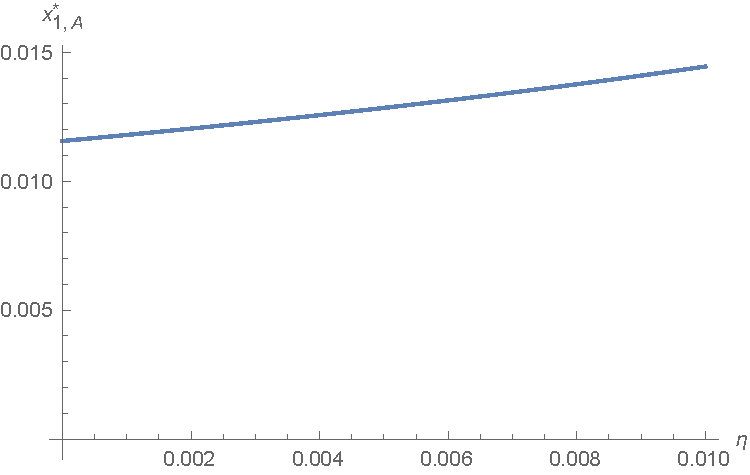
\includegraphics[width=0.32\textwidth]{Prob3/x1Aeta.pdf}}
		\subfigure[$\delta \in (1,2)$]{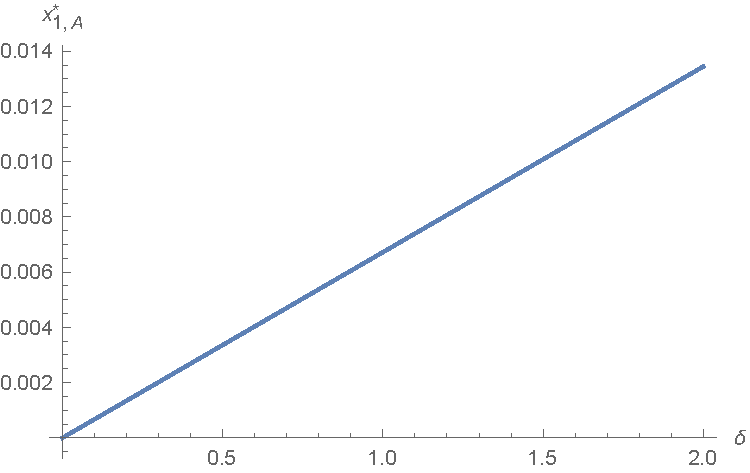
\includegraphics[width=0.32\textwidth]{Prob3/x1Adelta.pdf}}
		\subfigure[$\alpha \in (0, \min \{ 1/K_0, \theta/K_1 \} )$ ]{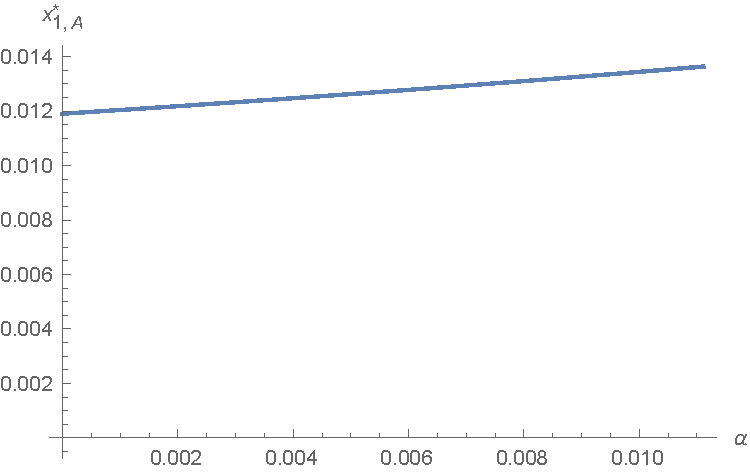
\includegraphics[width=0.32\textwidth]{Prob3/x1Aalpha.pdf}}
		\subfigure[$K_0 \in (0,1/\alpha)$]{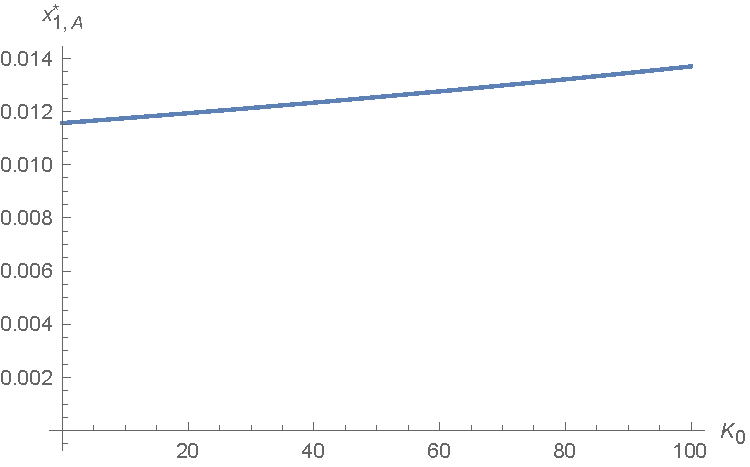
\includegraphics[width=0.32\textwidth]{Prob3/x1Ak0.pdf}}
		\subfigure[$K_1 \in (0,\theta/\alpha)$]{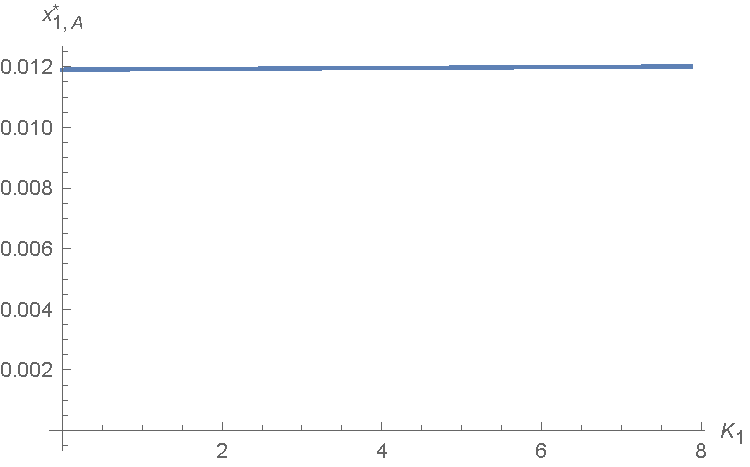
\includegraphics[width=0.32\textwidth]{Prob3/x1Ak1.pdf}}
		\subfigure[$\sigma \in (0,1)$]{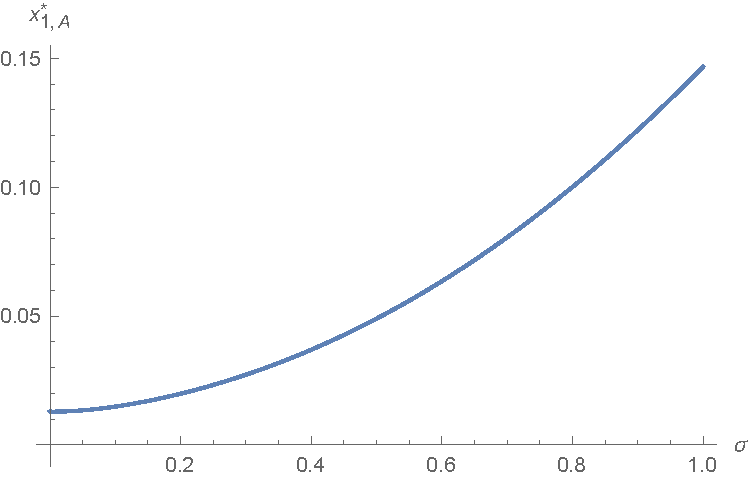
\includegraphics[width=0.32\textwidth]{Prob3/x1Asigma.pdf}}
		\subfigure[$r \in (0,\mu)$]{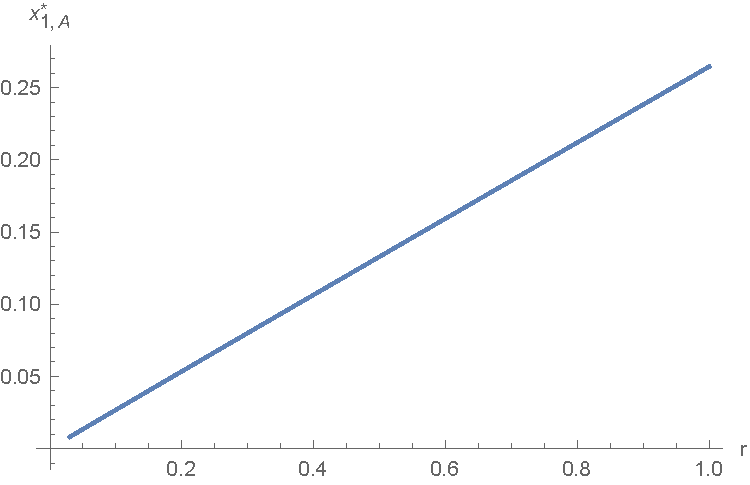
\includegraphics[width=0.32\textwidth]{Prob3/x1Ar.pdf}}
	\end{subfigmatrix}
	\caption{Threshold value $x^*_{1,A}$ with respect to the parameters with which it increases.}
	\label{fig:2_x1Ai}
\end{figure}

On Figure \ref{fig:2_x1Ai} (a) we observe that the larger the cannibalisation parameter, the later the firm is expected to adopt the new product, since a high demand needs to be observed such that the investment and associated costs of the simultaneous production are overcome. Recall that for quite large values of $\eta$, we are in the situation where is preferable to invest on the \textit{new} product, replacing immediately the \textit{old} one.

The linear relationship between $\delta$ and $x_{1,A}^*$, as presented on Figure \ref{fig:2_x1Ai} (b), comes immediately  by the threshold's expression. This is financially justified by the fact that a larger $\delta$ results on larger investmnet (sunk) costs and, therefore, the firm only invests when it could profit. 






Once again we observe on Figure \ref{fig:2_x1Ai} (f) that a growth uncertainty on the demand lead to the reprieve of the investment decision. 

Although we weren't able to deduce any analytical result concerning the interest rate, we obtain on Figure \ref{fig:2_x1Ai} (g) that, as already stated, its growth delays the investment decision.

%On Figure \ref{fig:2_x1Ai} we present numerical  comprove what was stated on Proposition \ref{3_propx1A}. We also add another one, regarding the discount rate $r$, for which we couldn't derive any analytical solution, but studying the behaviour of $x^*_{1,A}$ we conclude that it also increases with $r$.

\begin{figure}[!htb]
	\begin{subfigmatrix}{2}
		\subfigure[$\mu \in (0,r)$]{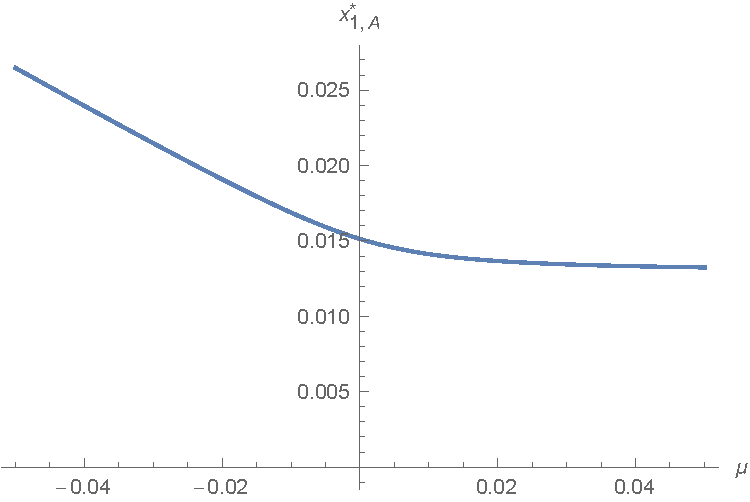
\includegraphics[width=0.32\textwidth]{Prob3/x1Amu.pdf}}
		\subfigure[$\theta \in (1,10)$]{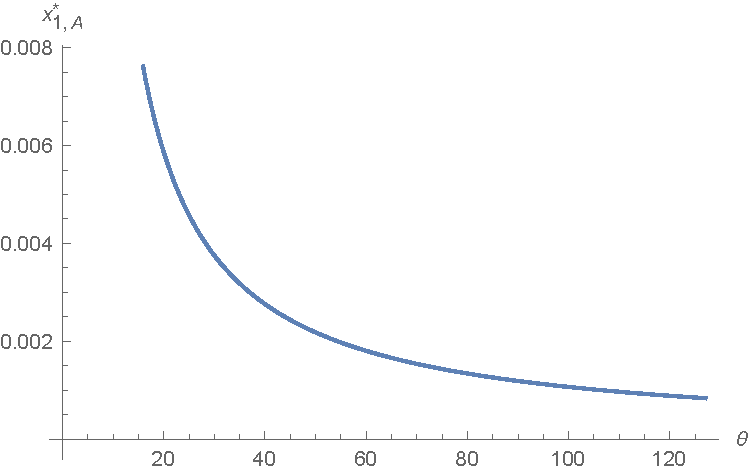
\includegraphics[width=0.32\textwidth]{Prob3/x1Atheta.pdf}}
	\end{subfigmatrix}
	\caption{Threshold value $x^*_{1,A}$ with respect to parameters with which it decreases.}
	\label{fig:2_x1Ad}
\end{figure}

On Figure \ref{fig:2_x1Ad} we present some plots that also comprove what was stated on Proposition \ref{3_propx1A}, but with respect to the parameters with which $x_{1,A}^*$ increases. Again, we add the plot concerning the drift parameter $\mu$, for which we couldn't derive any analytical solution, but studying the behaviour of $x^*_{1,A}$ we conclude that it also decreases with $\mu$.


\subsection{Demand threshold $x_{1,R}^*$}
\label{3_dmx1R}

All results come from Section \ref{2_bm} and thus they won't repeated here.



\subsection{Demand threshold $x_2^*$}
	\label{3_dmx2}
	
\begin{prop}
	\label{3_propx2}
	Decision threshold $x_2^*$ increases with $\sigma$ and decreases with $\eta, \ \alpha, \ K_0$ and $K_1$.
\end{prop}

\textbf{Proof:}

The results regarding parameters $\eta, \ \alpha, \ K_0$ and $K_1$ come immediately by the expression of $x_2^*$  \eqref{3:x2}.

Regarding $\sigma$, we obtain that
\begin{align*}
\frac{\partial x_2^* ( \sigma) }{\partial \sigma}=
\frac{(\alpha  K_0-1) (r-\mu) \left(-2 \mu ^2+\mu  \sigma ^2 \left(\phi+1\right)-2 r \sigma ^2\right)}{(d_1-1)^2 \eta  K_1 r \sigma ^5 \phi}>0
\end{align*}
where the denominator is positive since $d_1>1$, $\phi>0$  and the denominator is positive since $r>\mu$, $1-\alpha K_0>0$ and by noticing (again) that $-2 \mu ^2+\mu  \sigma ^2 \left(\phi+1\right)-2 r \sigma ^2<0 \Leftrightarrow \mu d_1-r<0$, which holds always, as previously showed in \eqref{mud1-r}.

%Regarding parameters $\mu$ and $r$, we obtained complex derivates, from which we couldn't deduce any analytical result. However, as it will be showed hereunder, $x^*_C$ behaves in a non-monotonic way with all of them.
\begin{flushright}
	$\square$
\end{flushright}

Considering the same parameters as in Section \ref{3_dmx1A}, we perform some numerical approximations concerning $x_2^*$.

\begin{figure}[!htb]
	\begin{subfigmatrix}{1}
		\subfigure[$\eta \in (0, \alpha )$ ]{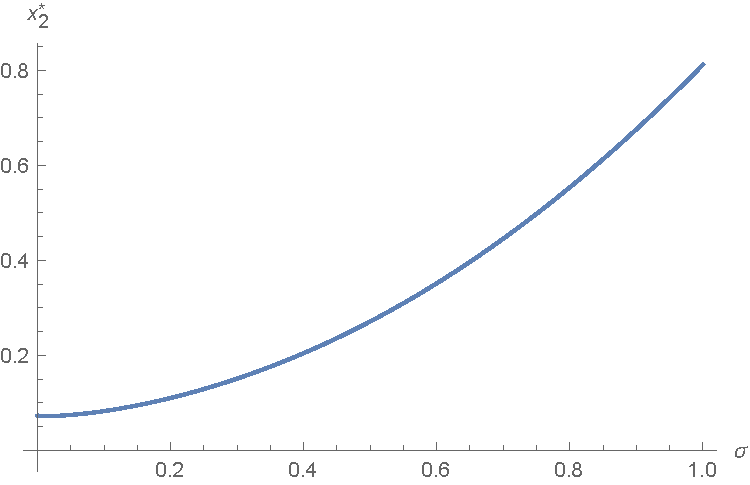
\includegraphics[width=0.45\textwidth]{Prob3/x2sigma.pdf}}
	\end{subfigmatrix}
	\caption{Threshold value $x^*_2$ with respect to parameters with which it increases.}
	\label{fig:2_x2i}
\end{figure}

From Figure \ref{fig:2_x2i} we comprove what was stated on Proposition \ref{3_propx2} regarding $\sigma$. 

We also obtained that the volatility $\sigma$ was the unique parameter we found to increase both thresholds $x_{1,A}^*$ and $x_2$. Note that by Section \ref{2_bm}, that the same holds for the threshold $x_{1,R}$. Thus we conclude that a situation where the demands shows to have a high volatility, both investment and replacement decisions tend to be postponed.

\begin{figure}[!htb]
	\begin{subfigmatrix}{6}
		\subfigure[$\eta \in (0, \alpha )$ ]{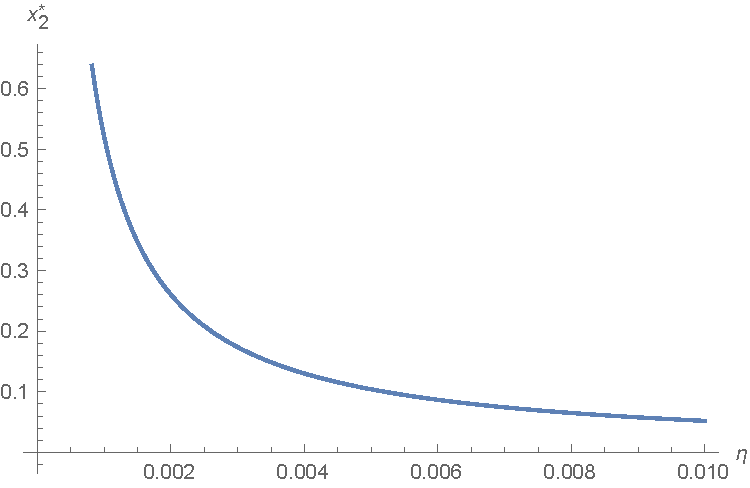
\includegraphics[width=0.32\textwidth]{Prob3/x2eta.pdf}}
		\subfigure[$\alpha \in (0, \min \{ 1/K_0, \theta/K_1 \} )$ ]{\includegraphics[width=0.32\textwidth]{Prob3/x2alpha.pdf}}
		\subfigure[$K_1 \in (0,\theta/\alpha)$]{\includegraphics[width=0.32\textwidth]{Prob3/x2k.pdf}}
		\subfigure[$K_0 \in (0,1/\alpha)$]{\includegraphics[width=0.32\textwidth]{Prob3/x2k0.pdf}}
		\subfigure[$r \in (0,\mu)$]{\includegraphics[width=0.32\textwidth]{Prob3/x2r.pdf}}
		\subfigure[$\mu \in (0,r)$]{\includegraphics[width=0.32\textwidth]{Prob3/x2mu.pdf}}
	\end{subfigmatrix}
	\caption{Threshold value $x^*_{1,A}$ with respect to parameters with which it decreases.}
	\label{fig:2_x2d}
\end{figure}

On Figure \ref{fig:2_x2d} we show how the threshold $x_2$ decreases with parameters stated on Proposition \ref{3_propx2}. We also add plots concerning the drift parameter $\mu$ and the discount rate $r$, for which we couldn't derive any analytical solution, but studying how $x^*_2$ behaves with them, we conclude that it also increases with $\mu$ and $r$, from which the behaviour showed may be generalized.
 % file "Thesis_Implementation.tex"
\cleardoublepage

\chapter{Sensibility analysis of optimal investment times}
\label{chapter:stoptime}



%%%%%%%%%%%%%%%%%%%%%%%%%%%%%%%%%%%%%%%%%%%%%%%%%%%%%%%%%%%%%%%%%%%%%%%%
\section{Introduction}
\label{section:stoptime_intro}

In this section we will analyse the optimal times to invest regarding the three different models developed on previous sections.

First, we will analyse some relevant measures - such as estimated mean, median and standard deviation - concerning the behaviour of optimal investment times with different initial demand values.

Secondly, we will analyse how the estimated mean of optimal investment times behaves with volatility and assess its relation with changes  either on the associated threshold value or optimal capacity level.

\section{Initial demand values $x_0$}
\label{section:x0}

\subsubsection{Methodology}










































%%%%%%%%%%%%%%%%%%%%%%%%%%%%%%%%%%%%%%
We analyse model by model, initially fixing relevant parameters to the considered situation, with the exception of the initial point $x_0$ - which is changed.

On the first and second situations, discussed on Chapters \ref{chapter:1} and \ref{chapter:2}, respectively, we consider $x_0$ to be incremented by \texttt{xStep}=0.0002 and to take values between 0.0002 and $3 \times  \texttt{xStep} + \lfloor \max{ \{ x_B^*, x_C^* \} } \rfloor]$. Such small values are considered due to the low investment triggering values associated to each of the models.


On the other side, since the magnitude of thresholds analysed on Chapter \ref{chapter:3}, is quite larger than the ones on previous two chapters, we consider the demand to be incremented by a larger step: \texttt{xStep}=0.002.
Recall that the most interesting situation on this chapter was obtained by considering $\eta<\eta^*$ \eqref{3_eta*} \footnote{For values $\eta \geq \eta^*$, we are in the same case as described on Chapter \ref{chapter:2}: we have an unique threshold which sets the transition from the production of the established product to the \textit{new} one.}, from which we would get an optimal investment time regarding the simultaneous production of established and \textit{new} products. Regarding the analysis of the optimal stopping time associated to $x_2^*$, we evaluate for a single initial demand value $x_{1,R}^*$, since this is the first instant, after investing when the demand reaching $x_{1,R}^*$.
%Considering the case when we invest on the \textit{new} product for a demand level $x$ greater than $x_{1,R}^*$, we would set the initial instant until it re



% on the analysis of the optimal investment time associated to $x^*_{1,A}$, we consider now $x_0$ to start at 0.002 and to be incremented, by \texttt{xStep}=0.002, until it achieves the value $3 \times  \texttt{xStep} + x_1,R^*$ and then

Note that $x_0$ is also taken to be greater than the correspondent thresholds. Considering those values, we numerically show that, whenever a firm is interested to invest in a market on which high demand levels are observed, it should immediately invest - obtaining a null expected waiting time.

%Regarding the first and second models, discussed on Chapters \ref{chapter:1} and \ref{chapter:2}, respectively, we consider $x_0 \in [0.0002, 3 \times  \texttt{xStep} + \lfloor \max{ \{ x_B^*, x_C^* \} } \rfloor]  ]$, in particular, values $x_{0_i}$ which are incremented $i$-th times by \texttt{xStep}=0.0002. Due to the noticeable difference of the order of magnitude of the thresholds on Chapter \ref{chapter:3}, we consider the interval of possible initial values to be $[0.002, 10 \times \texttt{xStep} +  \lfloor  x_{1,A}^* \rfloor] ]$, in particular, values $x_{0_i}$ which are incremented $i$-th times \texttt{xStep}=0.002.
		
%By fixing the firm's situation to analyse, we fix as well the respective demand threshold, for which, higher demand values, state that the investment should be done.



Using as input fixed initial demand values, steps and also demand's volatility and drift, function \texttt{generalStopTime} returns optimal investiment times' measures of interest. To a better understanding, outputs are plotted hereunder.
%We execute function \texttt{generalStopTime}, which, per each initial value, returns the measures we are interested on (mean, median or standard deviation) along with the initial demand value considered. To a better understanding, outputs are plotted hereunder.


The time step here can be chosen taking into account how drift and volatility of the demand process are estimated or in view of a certain time window.
Since these are mere illustrations concerning deduced models, we are able to choose an arbitrary time step. However, for the sake of a better understanding, we consider it to be one time unit.



%The time step we fix a time step of 1 time unit, but this value can be chosen to be in the same time scale as the estimated drift $\mu$ and volatility $\sigma$ of the GBM or regarding a certain time window. 


\subsubsection{Results}


For all the analysis performed, we consider the same set of parameters used on respective Comparative Statics sections. The only exception stands for volatility, which we increase to $\sigma=0.1$, in order to obtain results within a larger variability.


%Despite $\sigma$, these are the same values used on Chapter \ref{chapter:3}. Note that by choosing $\eta=0.007$, we have that $\eta< \eta^*$ and thus we are in the situation where the firm has two decisions to make: when it should invest and start the simultaneous production; when it should stop  the simultaneous production and produce solely the \textit{new} product.
%On Figure \ref{fig:stoptime_1} we can find the results obtained.

Results are presented on Figure \eqref{fig:stoptime_1}.
First we state that in every plot, the demand level that triggers the investment it is represented by a dashed line. As expected, for any initial value higher than the threshold,
% there is no waiting time until it's optimal to make the investment decision 
the firm is not expected to wait to decide
- not only the mean and median are null, so it is the standard deviation.


Observe that the smaller the initial value $x_0$, the higher (all) its respective measures are. 

Also, the higher threshold level, the longer (in average and median) the firm will need to wait until it should invest. This situation is particularly noticeable on results regarding Chapter \ref{chapter:1}.

The results concerning the mean and the median of the optimal investment times have an intuitive explanation: when starting with a small demand level (or considering an higher threshold), one expects to wait more time until the demand level reaches the threshold demand level, than when starting with an higher level (or with a smaller threshold). However the result concerning the standard deviation is not that obvious. It can arise due to the randomness of the GBM and its time increasing variance, respectively given by $Var(X_t)=X_0^2 e^{2\mu t}(e^{\sigma^2 t} -1), \ \forall t\geq0, \mu \geq 0$, which allows the sample path to be more diverse (either in observed states as in running lenght) and thus obtain also more distinct stopping times.
%Also, observe that for higher threshold levels, in average and median, the firm will need to wait more time until it is able to invest. This fact is particularly noticeable on the first two rows, whose results are taken with respect to the first situation (Section \ref{chapter:1}).
\pagebreak

\begin{figure}[!ht]
	\begin{subfigmatrix}{6}
		\subfigure[Mean \& Median of $\tau_B^*$ w.r.t. \eqref{eq:sistema} ]{\includegraphics[width=0.35\textwidth]{StopTime/1_BMtau.pdf}}
		\subfigure[Standard Deviation of $\tau_B^*$ w.r.t. \eqref{eq:sistema} ]{\includegraphics[width=0.35\textwidth]{StopTime/1_BMsd.pdf}}
		\subfigure[Mean \& Median of $\tau_C^*$ w.r.t. \eqref{eq:prob1_xC}]{\includegraphics[width=0.35\textwidth]{StopTime/1_COMtau.pdf}}
		\subfigure[Standard Deviation of $\tau_C^*$ w.r.t. \eqref{eq:prob1_xC}]{\includegraphics[width=0.35\textwidth]{StopTime/1_COMsd.pdf}}
		\subfigure[Mean \& Median of $\tau_B^*$ w.r.t. \eqref{2_xB} ]{\includegraphics[width=0.35\textwidth]{StopTime/2_BMtau.pdf}}
		\subfigure[Standard Deviation of $\tau_B^*$ w.r.t. \eqref{2_xB} ]{\includegraphics[width=0.35\textwidth]{StopTime/2_BMsd.pdf}}
		\subfigure[Mean \& Median of $\tau_C^*$ w.r.t. \eqref{eq:prob2_xC} ]{\includegraphics[width=0.35\textwidth]{StopTime/2_COMtau.pdf}}
		\subfigure[Standard Deviation of $\tau_C^*$ w.r.t. \eqref{eq:prob2_xC} ]{\includegraphics[width=0.35\textwidth]{StopTime/2_COMsd.pdf}}
		\subfigure[Mean \& Median of $\tau_{1,A}^*$ w.r.t. \eqref{eq:3_x1A}]{\includegraphics[width=0.35\textwidth]{StopTime/3_BMtau.pdf}}
		\subfigure[Standard Deviation of $\tau_{1,A}^*$ w.r.t. \eqref{eq:3_x1A} ]{\includegraphics[width=0.35\textwidth]{StopTime/3_BMsd.pdf}}
	\end{subfigmatrix}
	\caption{Sensibility analysis of estimated mean and median (leftmost column) and standard deviation (rigthmost column) of the optimal investment time for each of the three situations studied, regarding different initial values $x_0$.}
	\label{fig:stoptime_1}
\end{figure}

We highlight here, as well, the fact that the mean and the median of investment times is approximately equal, suggesting that the distribution of investment times is approximately symmetric.

On the last row we find the results concerning the optimal time to invest in a \textit{new} product and start to produce, simultaneously, the \textit{old} and \textit{new} products, as studied on Section \ref{chapter:3}. This result appears to be sparser (regarding the median) and more oscillated (regarding the standard deviation) than the others, due to the raise on the increment of the initial value (\texttt{xStep}), while the range of waiting times metrics isn't as wide as the ones obtained on previous situations. This might be seen also as a \textit{zoom} of the behaviour presented on previous plots.


Now, regarding the optimal time to stop the production of the established product, studied on Chapter \ref{chapter:3}, we obtain results presented on Table \ref{stoptime_t}.
\begin{table}[!htb]
	\caption{Sensibility analysis of estimated mean, median and standard deviation of optimal time to decide stop the production of the established product when considering an observed demand $x_{1,A}^*$.}
	\centering
	\begin{tabular}{ccc}
		Mean & Median & Standard Deviation \\ \hline
		5.49 & 5.00 & 0.77
	\end{tabular}
\label{stoptime_t}
\end{table}

Here we only consider the demand process to start at $x_{1,A}^*$, since this is the instant after which we are able to make the mentioned decision. Therefore, mean and median are taken considering as \textit{initial instant} the time at which the firm decides to invest in the new product and start the simultaneous production, that is, $\tau^*_{1,A}=\inf \{ t\geq 0: X_t \geq x^*_{1,A} \}$. Thus, the mean/median presented should be read as the mean/median time after the investment on the \textit{new} product was done. To obtain the estimated mean/median time for which the firm produces solely the \textit{new} product, one should add the value presented on Table \ref{stoptime_t} to the one obtained as the mean/median time to invest in the \textit{new} product, for a given initial demand value $x_0$.    

We obtain similar results as the ones stated above, in particular, that the mean and median of investment times is similar, suggesting that they have a symmetric distribution.


\section{Volatility sensibility analysis}

In this section we are interested to observe how optimal investment times behave with volatility.

\subsubsection{Methodology}

The results are mainly obtained recurring to function \texttt{estTau}, which has function \texttt{stopTimemod} included.

Considering a model and respective parameters fixed, \texttt{stopTimemod} simulates \texttt{NsamplePaths}=500 demand sample paths, recording the instant at each of them either reaches the demand threshold considered or reaches time \texttt{horizon}. Since it's not deterministic that all sample paths will reach the threshold, this last condition is crucial to assure that the algorithm runs in \textit{human-time}. On the results showed hereunder we consider \texttt{horizon}=1500 time units.

Function \texttt{estTau} calculates the mean of the investment times obtained by \texttt{stopTimemod} per each volatility level $\sigma_i$, which starts in 0.01 and it is incremented $i$-th times 0.01, until reaches \texttt{$\sigma$ Max}=0.5, that is $\sigma_i=0.01+i \times 0.01 \in [0.01,0.5]$.

We run \texttt{estTau} for each of the models studied - either benchmark or capacity optimization model - and considering two initial points $x_0 \in \{0.001, \ 0.01 \}$. We also evaluate as well the respective threshold values and optimal capacity in order to compare results obtained, based on their absolute value and variation.

In order to calculate the variation, we consider a partition of (0,0.5] with $0.5/0.01=50$ subintervals of the form $I_n=(\sigma_n, \sigma_{n-1}],\ n \in \{2,...,50\}$. Denoting the percentage of variation associated to the $I_n$ interval by $\triangle_n \%$, it follows that for $n \in \{2,...,50\}$ it is given by
$$\triangle_n \% = \frac{f(\sigma_n)-f(\sigma_{n-1})}{\sigma_n-\sigma_{n-1}} \times 100 \%,$$
with $f$ being any of the measures of interest - mean of investment times, demand threshold or optimal capacity -, which only depends on the volatility considered.




\subsubsection{Results}

Despite the initial demand value and volatility, the set of parameters considered, regarding each model, was the same as chosen in the previous section. We consider here as well a \texttt{timeStep} of one time unit. For each of the three situations studied, we present the graphical result and a table in which are numerically presented the diverse measures analysed regarding volatility increments of 0.05.

$\bullet$ \textbf{Situation on Chapter \ref{chapter:1}: firm has no products in the market and wants to introduce a new one}

On Figure \ref{fig:vol_1} we observe that both optimal investment times have a non-monotonic behaviour with the volatility. Even when the threshold level and the optimal capacity level increase with it.

One can also note that the optimal investment times for both benchmark and capacity optimization models increase significantly for volatilities $\sigma>0.35$. This effect is more significant when considering a smaller initial value $x_0$.

\begin{figure}[!ht]
	\begin{subfigmatrix}{3}
		\subfigure[(Estimated) mean of optimal investment times. ]{\includegraphics[width=0.32\textwidth]{StopTime/1_meantauSP500H1500.pdf}}
		\subfigure[Demand threshold. ]{\includegraphics[width=0.32\textwidth]{StopTime/1_x.pdf}}
		\subfigure[Optimal capacity level.]{\includegraphics[width=0.32\textwidth]{StopTime/1_k.pdf}}
	\end{subfigmatrix}
	\caption{Sensibility analysis of the (estimated) mean of optimal investment time, the threshold level and the optimal capacity level (referred on Chapter \ref{chapter:1}) with the volatility, regarding different initial values $x_0 \in \{0.001, \ 0.01\}$.}
	\label{fig:vol_1}
\end{figure}

Besides previous conclusions, on Table \ref{tab:vol_1}, we observe that the difference between $\tau_B^*$ and $\tau_C^*$, for $x_0=0.01$, is more noticeable than what it seems in Figure \ref{fig:vol_1}.

We found no relation between the behaviour of optimal investing times and threshold levels or optimal capacity. However it seems to exist an optimal volatility level such that the optimal investment time is the lowest. In this case, this optimal volatility level $\sigma^*$ seems to be $0.15 < \sigma^* < 0.25$ for $x_0=0.001$ and $\sigma^*<0.15$ for $x_0=0.01$.

\textcolor{red}{Referir esta parte do nível optimal de volatilidade? É verdade que a empresa não tem controlo sobre a volatilidade do nível de procura, contudo poderá escolher entre mercados com diferentes níveis de volatilidade. Mesma pergunta para todas as análises de volatilidade.}

\textcolor{red}{Manter tabela?}

\begin{table}[!ht]
	\centering
	\caption{Sensibility analysis of the (estimated) mean of optimal investment time, the threshold level and the optimal capacity level (referred on Chapter \ref{chapter:1}) with the volatility, regarding different initial values $x_0 \in \{0.001, \ 0.01\}$.}
	\begin{tabular}{c|ccccccccl}
		\hline
		\text{ $\sigma $ } & 0.05 & 0.1 & 0.15 & 0.2 & 0.25 & 0.3 & 0.35 & 0.4 \\ \hline
		$K^*$ & 381.04 & 395.08 & 410.92 & 425.39 & 437.62 & 447.66 & 455.80 & 462.41 \\
		$x_B^*$ & 0.012 & 0.013 & 0.015 & 0.017 & 0.020 & 0.023 & 0.027 & 0.032 \\
		$x_C^*$ & 0.017 & 0.019 & 0.022 & 0.027 & 0.032 & 0.038 & 0.045 & 0.053 \\ \hline
	   $\overline{\tau _B}$ & 67.64 & 58.71 & 53.64 & 52.22 & 52.46 & 57.49 & 63.97 & 106.98 & \rdelim\}{2}{0.05mm}[$x_0=0.001$]  \\
		$\overline{\tau _C}$ & 78.21 & 68.43 & 63.82 & 63.94 & 65.55 & 70.66 & 90.09 & 193.65 \\ \hline
		$\overline{\tau _B}$ & 4.29 & 5.26 & 6.48 & 7.81 & 9.53 & 10.25 & 11.90 & 14.154 &	\rdelim\}{2}{0.05mm}[$x_0=0.01$] \\
		$\overline{\tau _C}$ & 13.88 & 12.89 & 13.40 & 14.92 & 15.53 & 16.93 & 19.77 & 23.11
	 \\ \hline
	\end{tabular}
\label{tab:vol_1}
\end{table}


Regarding the observed variation of considered parameters, on Figure \ref{fig:var_1}, we verify what was already stated. 
For volatility values bigger than 0.35, we observe changes up to 140\% on the variation of optimal investment times' mean, making the growth of all other parameters to seem despicable, as can be seen in the leftmost side. 
However when we focus on volatility values smaller than 0.35, the mean of optimal investment times doesn't vary significantly, having a variation in magnitude smaller than 4\%, as can be seen in the rightmost side.



\begin{figure}[!ht]
	\begin{subfigmatrix}{2}
		\subfigure[Variation of parameters of interest for volatilities $\sigma \in (0,0.5)$. ]{\includegraphics[width=0.4\textwidth]{StopTime/1_varSP500H1500.pdf}}
		\subfigure[Variation of parameters of interest for volatilities $\sigma \in (0,0.35)$. ]{\includegraphics[width=0.4\textwidth]{StopTime/1_varSP500H1500_35.pdf}}
	\end{subfigmatrix}
	\caption{Variation of (estimated) mean of optimal investment time, the threshold level and the optimal capacity level (referred on Chapter \ref{chapter:1}) with the volatility, regarding different initial values $x_0 \in \{0.001, \ 0.01\}$.}
	\label{fig:var_1}
\end{figure}





$\bullet$ \textbf{Situation on Section \ref{chapter:2}: firm has an established product and want to introduce a new one, replacing the other one}


On Figure \ref{fig:vol_2} we can observe that conclusions stated before hold. Optimal investment times have a non-monotonic behaviour with the volatility and they seem not to be related neither with threshold values or the optimal capacity level. 

\begin{figure}[!ht]
	\begin{subfigmatrix}{3}
		\subfigure[(Estimated) mean of optimal investment times. ]{\includegraphics[width=0.32\textwidth]{StopTime/2_meantauSP500H1500.pdf}}
		\subfigure[Demand threshold. ]{\includegraphics[width=0.32\textwidth]{StopTime/2_x.pdf}}
		\subfigure[Optimal capacity level.]{\includegraphics[width=0.32\textwidth]{StopTime/2_k.pdf}}
	\end{subfigmatrix}
	\caption{Sensibility analysis of the (estimated) mean of optimal investment time, the threshold level and the optimal capacity level (referred on Chapter \ref{chapter:2}) with the volatility, regarding different initial values $x_0 \in \{0.001, \ 0.01\}$.}
	\label{fig:vol_2}
\end{figure}

Once again, confronting the results on Figure \ref{fig:vol_2} with the ones presented on Table \ref{tab:vol_2}, we observe that the idea of having an optimal volatility level might be also valid again.  In this case, the optimal volatility level $\sigma^*$ seems to be $0.15 < \sigma^* < 0.25$ for both initial values $x_0=0.001$ and $x_0=0.01$.


\begin{table}[!ht]
	\centering
	\caption{Sensibility analysis of the (estimated) mean of optimal investment time, the threshold level and the optimal capacity level (referred on Chapter \ref{chapter:2}) with the volatility, regarding different initial values $x_0 \in \{0.001, \ 0.01\}$.}
	\begin{tabular}{c|ccccccccl}
		\hline
		\text{ $\sigma $ } & 0.05 & 0.1 & 0.15 & 0.2 & 0.25 & 0.3 & 0.35 & 0.4 \\ \hline
		$K^*$ & 406.62 & 416.81 & 428.59 & 439.60 & 449.10 & 457.01 & 463.51 & 468.84  \\
		$x_B^*$ & 0.022 & 0.024 & 0.028 & 0.033 & 0.038 & 0.045 & 0.052 & 0.060  \\
		$x_C^*$ & 0.021 & 0.024 & 0.028 & 0.033 & 0.039 & 0.047 & 0.055 & 0.064 \\ \hline
		$\overline{\tau _B}$ & 86.86 & 76.4 & 71.57 & 65.01 & 68.18 & 73.59 & 84.79 & 203.85  & \rdelim\}{2}{0.05mm}[$x_0=0.001$]  \\
		$\overline{\tau _C}$ & 86.45 & 75.33 & 69.36 & 67.75 & 71.57 & 76.08 & 99.44 & 194.35 \\ \hline
		$\overline{\tau _B}$ & 20.94 & 18.04 & 18.04 & 17.19 & 17.37 & 19.55 & 22.19 & 25.88  &	\rdelim\}{2}{0.05mm}[$x_0=0.01$] \\
		$\overline{\tau _C}$ & 20.34 & 18.69 & 18.18 & 17.94 & 19.88 & 21.21 & 22.04 & 23.02  \\ \hline
	\end{tabular}
\label{tab:vol_2}
\end{table}


Regarding the observed variation of considered parameters, on Figure \ref{fig:var_2}, we find a similar situation to the one described above.
This time, the mean of optimal investment times vary up to 160\%  for volatility values bigger than 0.35, and vary up to 4\%, for volatility values smaller than 0.35.


\begin{figure}[!ht]
	\begin{subfigmatrix}{2}
		\subfigure[Variation of parameters of interest for volatilities $\sigma \in (0,0.5)$. ]{\includegraphics[width=0.4\textwidth]{StopTime/2_varSP500H1500.pdf}}
		\subfigure[Variation of parameters of interest for volatilities $\sigma \in (0,0.35)$. ]{\includegraphics[width=0.4\textwidth]{StopTime/2_varSP500H1500_35.pdf}}
	\end{subfigmatrix}
	\caption{Variation of (estimated) mean of optimal investment time, the threshold level and the optimal capacity level (referred on Chapter \ref{chapter:2}) with the volatility, regarding different initial values $x_0 \in \{0.001, \ 0.01\}$.}
	\label{fig:var_2}
\end{figure}




$\bullet$ \textbf{Situation on Chapter \ref{chapter:3}: firm has an established product and want to introduce a new one, allowing a phase of simultaneous production}


On Figure \ref{fig:vol_3}, there are represented both estimated means of optimal investment times upon which the firm should invest in the \textit{new} product and start the simultaneous production of the \textit{old} and \textit{new} products, given initial demand values $x_0 \in \{ 0.001, \ 0.01 \}$, and the estimated mean of optimal time to suppress the production of the old product and start solely to produce the \textit{new} product, considering the starting demand value to be $x_{1,A}^*$. We observe that this time none of the estimated means seem to vary significantly with the volatility level considered.


\begin{figure}[!ht]
	\begin{subfigmatrix}{3}
		\subfigure[(Estimated) mean of optimal investment times.]{\includegraphics[width=0.32\textwidth]{StopTime/3_meantau.pdf}}
		\subfigure[Demand threshold.]{\includegraphics[width=0.32\textwidth]{StopTime/3_x.pdf}}
		\subfigure[Variation of parameters of interest for volatilities $\sigma \in (0,0.5)$.]{\includegraphics[width=0.32\textwidth]{StopTime/3_var.pdf}}
	\end{subfigmatrix}
	\caption{Sensibility analysis of the (estimated) mean of optimal investment time, the threshold level and the optimal capacity level (referred on Chapter \ref{chapter:3}) with the volatility, regarding different initial values $x_0 \in \{0.001, \ 0.01\}$.}
	\label{fig:vol_3}
\end{figure}

Confronting both results present on Figure \ref{fig:vol_3} and Table \ref{tab:vol_3}, we note that none of the estimated means seem to vary with the value of the correspondent threshold level for any level of volatility considered. In this situation, there is no evidence of an optimal volatility level that evidences a minimum investment time, as it happened in previous analysis.


\begin{table}[!ht]
	\centering
	\caption{Sensibility analysis of the (estimated) mean of optimal investment time, the threshold level and the optimal capacity level (referred on Chapter \ref{chapter:3}) with the volatility, regarding different initial values $x_0 \in \{0.001, \ 0.01\}$.}
	\begin{tabular}{c|ccccccccc}
		\hline
		\text{ $\sigma $ } & 0.05 & 0.1 & 0.15 & 0.2 & 0.25 & 0.3 & 0.35 & 0.4 \\ \hline
		$x_{1,A}^*$ & 1.092 & 1.101 & 1.116 & 1.136 & 1.161 & 1.190 & 1.224 & 1.261   \\
		$x_2^*$ & 6.518 & 6.572 & 6.659 & 6.779 & 6.928 & 7.104 & 7.306 & 7.530  \\ \hline
		$\overline{\tau _{1,A}}$ & 16.08 & 16.18 & 16.13 & 16.07 & 16.06 & 16.34 & 16.34 & 16.64  & \rdelim\}{1}{0.05mm}[$x_0=0.001$] \\
		$\overline{\tau _{1,A}}$ & 10.92 & 11.00 & 11.01 &  11.08 & 11.10 & 1.10 & 11.27 & 11.53 & \rdelim\}{1}{0.05mm}[$x_0=0.001$]  \\ \hline
		$\overline{\tau _2}$ & 4.48 & 4.50 & 4.54 & 4.56 & 4.65 & 4.55 & 4.49 & 4.63   \\ \hline
	\end{tabular}
\label{tab:vol_3}
\end{table}






 We tried different values, in particular, bigger, of \texttt{NsamplePaths} and \texttt{horizon}. However, by results obtained, by considering bigger values for referred parameters, we raise (considerably) the computational running time but it doesn't seem to bring more precise results.
 
\cleardoublepage

\chapter{Value of the project: the influence of the number of innovation jumps}
\label{chapter:max}



%%%%%%%%%%%%%%%%%%%%%%%%%%%%%%%%%%%%%%%%%%%%%%%%%%%%%%%%%%%%%%%%%%%%%%%%
\section{Introduction}
\label{section:max_intro}

On all previous chapters we kept our focus on a timeline starting at the instant a desired innovation level $\theta$ was achieved and hence, ignoring all what happened before it, we 
studied the value function and the demand value that triggers the investment associated to three different contexts - entering the market with an innovative product; introducing a new product with the immediate replacement of the \textit{old} one; introducing of a \textit{new} product with the possibility of immediate replacement of the \textit{old} one or simultaneous production followed by the replacement of the \textit{old} product).
% -, by setting time to start when
% while considering a fixed level of innovation $\theta$.

On this chapter we are interested to calculate the maximized expected value function, associated to each of the three contexts, with respect to the R\&D investment made and taking into account the waiting time until the innovation breakthrough takes place.
This allows us to state a relation between the R\&D investment and the time a firm needs to wait until it is in a favourable situation to invest.
%give a weight depending on the time we need to wait until we are able to introduce the \textit{new} product.

%Here we will consider the case when $\theta$ is achieved at the next jump and, the generalization of it, when only at the $n$-th jump ($n \in \mathds{N}$) we obtain the desired threshold $\theta$.


Innovation levels are assumed to increase by jumps. Therefore the innovation process
%As stated in Introduction, recall that the innovation process 
$\Theta=\{ \theta(t), \ t \geq 0 \}$ is defined as an homogenous Compound Poisson Process with constant rate given by $\lambda(R)=R^\gamma$ with $R$ corresponding to the investment in the R\&D department, and $\gamma$ a sensibility parameter taking values in $(0,1]$.

%The higher the R\&D investment, the smaller the expected waiting time until the desired level $\theta$ occurs is, so the higher the value function will be.

Note that R\&D investment (R) is different from investment costs ($\delta K$): the first influences directly the innovation $\Theta$, while the second is related with costs the firm needs to incur to adapt its production to the new technology level.
For example, R\&D costs can be related with scientist wages and laboratory equipment while investment costs can be related to new equipment the firm needs to purchase or formation necessary to its employees, in order to adapt to the new technology level.



The innovation process can be then expressed as
$$\theta_t=\theta_0+uN_t, \ t\geq 0.$$ 
with $\theta_0$ denoting the state of technology at the initial point in time, $u>0$ a fixed jump size and $\{ N_t, \ t \geq 0 \}$ the jump process which follows a Poisson Process with rate $\lambda(R)$. 
%Note that the higher the innovation threshold $\theta$ desired, the later the innovation will occur (in average), but the higher the demand for the \textit{new} product will be.

Considering now $S_n$ to be the random variable that represents the waiting time until the $n$-th jump is observed, accordingly to \cite{ross}, $S_n$ follows an Erlang distribution with shape parameter $n$ and rate parameter $\lambda(R)$, the same as in the jump process, that is,
$$S_n=\min \{t\geq 0: N(t)=n \} \sim Erlang(n,\lambda(R)).$$

It immediately follows that the expected waiting time for the $n$-th jump to be reached is given by $\mathds{E}(S_n)=\frac{n}{\lambda(R)}$, meaning that the larger the R\&D investment, the sooner the $n$-th jump is expected to be observed. Also, note that, if there is no investment on R\&D, the jumps are supposed to occur at a null rate ($\lambda(0)=0$), resulting in a infinite expected waiting time.
%Accordingly to \cite{ross}, we have that $S_n$ is distributed according to Erlang distribution with shape parameter $n$ and rate parameter being the same as the Poisson Process, that is, $\lambda(R)$. From this it follows that the expected waiting time for the $n$-th jump to be reached is given by $\mathds{E}(S_n)=\frac{n}{\lambda(R)}.$ Thus, the higher the investment, the bigger the quantity of jumps observed is. Note that, in the situation in which there is no R\&D investment, there is also no evolution in the innovation process, since it implies a null rate $\lambda(0)=0$ followed by an infinite waiting time for any amount of jumps wanted to be observed.

%Note from previous deduced expressions of value function that none of them depend on the R\&D investment $R$. This one only influences the innovation process. Therefore, as it will be showed in the next sections, this is a standard maximization problem, in which we will want to maximize the expected value function with respect to the R\&D investment $R$.
% the work made in the last chapter of \cite{rita}, since our investment decision is not done based on a certain optimal innovation level, but, instead, based on optimal demand level(s), only after a threshold innovation level $\theta$ is reached.



Therefore, in this chapter we are interested to study how the complete value of the project - reflecting R\&D investment so as the innovative product investment - is affected by the R\&D investment and the number of jumps needed until it is favourable to invest on the innovative product. First we focus on the situation when the innovation breakthrough happens within one innovation jump and then we generalise this scenario, by considering the breakthrough to occur within $n\in\mathds{N}$ jumps.


We close this introduction, highlighting the fact that every investment value function previously deduced is independent of the R\&D investment, solely on the technology level $\theta$.

%%%%%%%%%%%%%%%%%%%%%%%%%%%%%%%%%%%%%%%%%%%%%%%%%%%%%%%%%%%%%%%%%%%%%%%%
\section{One jump}
\label{section:max_1jump}

We start with the simplest case: the desired innovation level $\theta$ is reached within one jump.
Therefore $S_1$ denotes the random variable associated to the waiting time until the jump occurs and it is such that
$$S_1 \sim \text{Erlang}(1,\lambda(R)) \overset{d}{=} \text{Exponential}(\lambda(R)).$$

We also will denote here $F$ to be the value function associated to an investment situation and $V$ to be the maximized value of the investment project given by
\begin{equation}
	V(x)=\max_R \mathds{E} [ e^{-rS_1}F(x)-R]\geq 0
	\label{max_V}
\end{equation}

It consists on the maximized expected value of the investment on a new technology minus R\&D costs associated. Note that, since we assumed the timeline of $F$ to start when the innovation breakthrough occurs ($S_1$), we discount its value to the time the R\&D investment is made and consider $x$ to be the demand value expected to observe at $S_1$.

Note that, having calculated $F$, all terms are deterministic with the exception of the waiting time until the breakthrough occurs. Therefore, we need to calculate the expected value of the whole investment.
%and corresponding to the maximized expected discounted value function minus the R\&D investment needed to be made. Recall that, in the previous sections, we deduced all the value functions by setting the initial time to be the time at the innovation threshold $\theta$ is reached. Therefore in order to have the real value, we need to discount it to the time when the jump happens, that is, $S_1$. Also, since the jumps are governed by a stochastic process (and thus they are random), we need to calculate the expected value of the discounted value function. Since the R\&D investment $R$ is deterministic, it could be inside or outside the expected value (but for the sake of simplicity we decided to include it when calculating the expectation).

In order to estimate the function $V$, one could have made it directly through stochastic simulations, using Monte Carlo methods for instance. However we here we deduced an analytical result, which is stronger than any estimation made.
%preferred to deduce an analytical result, since its stronger than any estimation made. 


Taking into account tht the epxectation is with respect to $S_1$, we obtain
%Coming back to the expression of $V$ in \eqref{max_V}, and by considering the expectation with respect to $S_1$ we obtain that it follows
\begin{align}
 V(x)&=\max_R  \left\{ \int_0 ^\infty f_{S_1}(t) e^{-rt} F(x) dt -R \right\} \nonumber \\
 &=\max_R  \left\{ \int_0 ^\infty \lambda(R) e^{-\lambda(R)t} e^{-rt} F(x) dt -R \right\} \label{max_V2}
\end{align}
where $f_{S_1}$ corresponds to the probability density function of an Exponential distribution with parameter $\lambda(R)$. %, associated to the random variable $S_1$.

Since, as previously written (and deduced), none of the value functions studied depend on the R\&D investment or the time at they are evaluated, only on the demand level observed at the breakthrough, $F$ never depends on $R$ or $t$. Therefore the integral on \eqref{max_V2} can be solved, leading to
\begin{equation}
V(x)=\max_R \left\{ \frac{\lambda(R)}{\lambda(R)+r} F(x) -R \right\}=\max_R \left\{ \frac{R^\gamma}{R^\gamma+r} F(x) -R \right\},
\label{max_V3}
\end{equation}
which is a maximization problem with respect to the R\&D investment $R$. Since by \eqref{max_V}, $V$ cannot be negative it follows that the restriction
\begin{equation}
R^\gamma F(x) - (R^\gamma+r)R \geq 0 \ \Leftrightarrow  F(x) \geq \frac{R^\gamma+r}{R^{\gamma-1}}
	\label{max_rest}
\end{equation}
must always be verified.

The optimal value of the investment to be made, from now on denoted by $R^*$, is found by analyzing the first and the second partial derivatives of the expression to maximize, that is,
\begin{align}
\frac{\partial}{\partial R} \left( \frac{R^\gamma}{R^\gamma+r} F(x) -R \right) &= \frac{\gamma R^{\gamma-1}F(x)r-(R^\gamma+r)^2}{(R^\gamma+r)^2} \label{max_ddR}\\
\frac{\partial^2}{\partial R^2} \left( \frac{R^\gamma}{R^\gamma+r} F(x) -R \right) &=
-\frac{F(x) \gamma r R^{-2+\gamma}(r-\gamma r+(1+\gamma)R^\gamma)}{(R^\gamma+r)^3}\leq 0.
\label{max_d2dR2}
\end{align}

Note that, since $\gamma \in (0,1]$, $F(x)\geq0 \ \forall x$ and $r, \ R >0$, the second partial derivative with respect to $R$ \eqref{max_d2dR2} is always negative. Hence the expression to be maximized in \eqref{max_V3} corresponds to a concave function, meaning that we are always able to find a value $R^*=\arg \underset{R}{\max} \left\{ \frac{R^\gamma}{R^\gamma+r} F(x) -R \right\}$.

Regarding the set of possible values for $\gamma$ and their interest, we consider two different cases.

Firstly we analyse the solution considering $\gamma=1$, meaning that jumps happen at a rate equal to the investment made. This is the only case for which
% although this implies that the jump's rate is equal to $R$, it is, nevertheless, an important case since it was the only one for which
we were able to obtain an analytical solution. Secondly we analyse other possible values $\gamma \in (0,1)$, whose results are only able through a numerical solver and software \texttt{Mathematica}.

The case $\gamma=0$ is not here considered due to its lack of relevance for the problem.
% , regarding the problem in hands. Note that 
Since $\gamma=0 \ \Rightarrow \ \lambda(R)=1,$ the innovation rate is not influenced by the R\&D investment made.

%that is, considering $\gamma=0$, the innovation rate is not influenced by the size of the R\&D investment made (which is not compatible with the real life).

$\bullet$ \textbf{Case I:} $\gamma=1 \Leftrightarrow \lambda(R)=R$

Analysing the roots of the first partial derivative in order to investment parameter $R$, we get a quadratic polynomial, whose zeros are given by
%which we can calculate obtain the expression of the zeros, obtaining
%$$   \frac{\partial}{\partial R} \left( \frac{R}{R+r} F(X) -R \right) = \frac{ F(X)r-(R+r)^2}{(R+r)^2}=0 $$
%$$   \Rightarrow F(X)r-(R^2+2rR+r^2)=0$$
$$  R=-\sqrt{F(x)r}-r \  \vee \ R=\sqrt{F(x)r}-r$$

Since it is not possible to have negative investment, we discard the leftmost solution.
%The first solution is not admissible, since it's not possible to have negative investment ($R>0$).

The second solution is admissible, since it is always true that
\begin{align}
 \sqrt{F(x)r}-r  \ &\underset{\eqref{max_rest}}{\geq} \ \sqrt{(R+r)r}-r \geq 0 \nonumber \\
 &\Leftrightarrow rR+r^2-r^2=rR\geq 0.
 %= \sqrt{rR+R^2}-r  \ \underset{\triangle}{\geq} \ \sqrt{rR}+\sqrt{R^2}-r=\sqrt{rR},
\end{align}

%On account of the negativity 
%Concerning the second partial derivative \eqref{max_d2dR2}, we obtain that, if \eqref{max_rest} holds, then the optimal R\&D investment to be made corresponds to
Thus, if condition \eqref{max_rest} holds, the optimal investment is given by
\begin{equation}
R^*=\max_R V(x)= \sqrt{F(x)r}-r.
\end{equation}


$\bullet$ \textbf{Case II:} $\gamma \in (0,1) $

Considering now $\gamma \in (0,1) $ and taking into account expression \eqref{max_ddR}, potential maximizers of $V$, %stationary points 
will be found by calculating the roots of the following polynomial
\begin{equation}
R^{\gamma-1}F(x)r-R^{2\gamma}-2rR^\gamma-r^2=0.
 \label{max_root}
\end{equation}


From condition \eqref{max_d2dR2} it follows that the maximizer $R^*$ is such that it verifies \eqref{max_rest} and \eqref{max_root}.

Unfortunately, we are not able to solve \eqref{max_root} analytically for any value $\gamma \in (0,1) $. However, using software \texttt{Mathematica}, we performed some numerical illustrations for values $\gamma \in (0,1)$ presented in Section \ref{maximexp_cs}.


\section{Multiple jumps}
\label{section:max_jumps}

Now we it take another step and generalize previous idea by considering that the desired innovation level $\theta$ is reached at the $n$-th innovation jump.
Therefore we consider $S_n$ to be the random variable associated to the waiting time until the $n$-th jump occurs and it is such that
$$S_n \sim \text{Erlang}(n,\lambda(R)).$$

Note that by considering $n=1$, we are at the situation analysed in the previous section.

For the sake of simplicity we keep the same notation as before, where $F$ denotes the value function associated to a certain investment situation and $V$ the maximized expected discounted value function minus the R\&D investment needed to be made, is now given by
\begin{align}
V_n(x)&=\max_R \mathds{E} [ e^{-rS_n}F(x)-R] \nonumber \\
&=\max_R  \left\{ \int_0 ^\infty f_{S_n}(t) e^{-rt} F(x) dt -R \right\} \nonumber \\
&=\max_R  \left\{ \int_0 ^\infty \frac{\lambda(R)^n t^{n-1}}{(n-1)!} e^{-\lambda(R)t} e^{-rt} F(x) dt -R \right\}
\label{max_2V}
\end{align}
where $f_{S_n}$ corresponds to the probability density function of an Erlang with shape parameter $n$ and rate parameter $\lambda(R)$.
%, associated to the random variable $S_n$.

Considering $W$ to be a random variable such that $W \sim \text{Erlang}(n, \lambda(R)+r)$ and $f_W$ the correspondent probability density function, the integral above can be simplified as it follows
\begin{align}
\int_0 ^\infty \frac{\lambda(R)^n t^{n-1}}{(n-1)!} e^{-\lambda(R)t} e^{-rt} F(x) dt &=
\frac{\lambda(R)^n}{(\lambda(R)+r)} F(x) \int_0 ^\infty \frac{(\lambda(R)+r)^n t^{n-1}}{(n-1)!} e^{-t(\lambda(R)+r)^n)} dt \nonumber \\
&=\left( \frac{\lambda(R)}{\lambda(R)+r}\right)^n F(x)  \int_0 ^\infty f_W(t) \ dt \nonumber \\
&=\left( \frac{\lambda(R)}{\lambda(R)+r}\right)^n F(x). \label{max_2V2}
\end{align}

Plugging the resultant expression \eqref{max_2V2} in \eqref{max_2V}, we obtain that $V_n$ corresponds to a standard maximization problem given by
\begin{equation}
V_n(x)=\max_R \left\{ \left( \frac{\lambda(R)}{\lambda(R)+r}\right)^n F(x)-R \right\}=\max_R \left\{ \left( \frac{R^\gamma}{R^\gamma+r}\right)^n F(x)-R \right\}.
	\label{max_2V3}
\end{equation}

Since $V_n$ is expected to be greater or equal to 0 $\forall n \in \mathds{N}$, the following restriction must hold
\begin{align}
R^{\gamma n} F(x)-R(R^\gamma + r)^n \geq 0 \  \Leftrightarrow \ F(x) \geq \frac{(R^\gamma+r)^n}{R^{\gamma n -1}}.
\label{max_2rest}
\end{align}


The optimal investment to be made, considering that at the $n$-th jump we achieve the desired breakthrough level $\theta$ and from now on denoted by $R^*_n$, is found by analysing the first and the second partial derivatives of the expression to maximize, that is,
\begin{align}
\frac{\partial}{\partial R} \left( \left( \frac{R^\gamma}{R^\gamma+r}\right)^n F(x)-R \right) &= \frac{\gamma  F(x) n r \left(\frac{R^{\gamma }}{r+R^{\gamma }}\right)^n-r R+R^{\gamma +1}}{r R+R^{\gamma +1}} \label{max_2ddR}\\
\frac{\partial^2}{\partial R^2} \left( \left( \frac{R^\gamma}{R^\gamma+r}\right)^n F(x)-R\right) &=
\frac{\gamma  F(x) n r \left(\frac{R^{\gamma }}{r+R^{\gamma }}\right)^n \left(r (\gamma  n-1)-(\gamma +1) R^{\gamma }\right)}{R^2 \left(r+R^{\gamma }\right)^2}.
\label{max_2d2dR2}
\end{align}

Due to the high complexity of both expressions above represented, we are not able to deduce an expression for stationary points neither to assess if the second partial derivative is negative.

Thus stationary points are numerically calculated. If, when evaluated at \eqref{max_2d2dR2}, they return a negative value, they are relative maximums (otherwise they are relative minimums on which we are not interested). The optimal investment $R^*$ is selected among all relative maximums as the one which maximizes $V_n$.
%This time we are not able to deduce if the second partial derivative is negative. Thus, in order to check if a stationary point is a minimum or a maximum, we will replace its value on expression \eqref{max_2d2dR2}. If it leads to a negative value, it will be considered as a relative maximum. $R^*$ will be selected among all these values to be one that maximizes the most $V_n$.

%We are not even able to find any stationary point analytically, due to the complexity of \eqref{max_2ddR}.













\section{Comparative Statics}
\label{maximexp_cs}

In this Section we assess how optimal investment $R^*$, its associated rate jump $\lambda(R^*)$ and optimal value function $V_n$ behave with the number of jumps considered $n$ and sensibility chosen $\gamma$.


Since we are not abe to deduce any analytical expression regarding the optimal R\&D investment, we develop a function that returns an approximation to the optimal R\&D investment, for a fixed situation. This function is presented in Appendix under the name \texttt{calcR}.

In view of the numerical experiments, by the independence of $F$ on parameters $R$ and $\gamma$, we consider it to be fixed and to take the value of 10. The discount rate is fixed at $r=0.05$ and $\gamma$ is considered to start at $0.05$ and incremented $0.05$ until it reaches 1.

%As stated in Section \ref{section:max_jumps}, we are not able to find an analytical expression regarding the roots of expression \eqref{max_2ddR} and hence we are not able to derive ana analytical expression for the optimal R\&D investment $R^*$. However, we developed a function that, given a certain parameter $\gamma$ and an amount of jumps $n$ and considering a fixed discount rate $r$ and the value function evaluated for an initial demand level $x$ $F(x)$, calculates numerically the R\&D investment that optimizes expression \eqref{max_ddR}, that leads to function $V_n$. This function is presented in Appendix by the name \texttt{calcR}. All of the next results were obtained using it.

%%The following parameters were considered regarding all the next results:
%\begin{itemize}
%	\item $r=0.05$;
%	\item $F(X)=10$;
%\end{itemize}
%We also considered different values of $\gamma \in (0,1]$, starting in 0.05 and, incremented by 0.05, until 1.

%Note on expression \eqref{max_2V3}, since $F(x)$ is not influenced by $\gamma$ or $R$, it can be seen as a constant term representing the value of the project assuming an innovation level $\theta$, which is yet to come. Hence we are able to proceed with our numerical approximations.

We start analysing the case when a firm is in a favourable position to invest after an innovation jump (this is the case when $n=1$).

\begin{figure}[!htb]
	\begin{subfigmatrix}{2}
		\subfigure[$R \in {(0,1]} $ and $\gamma \in {(0,1]} $. ]{\includegraphics[width=0.45\textwidth]{Jumps/RgammaV.pdf}}
		\subfigure[A particular case: $\gamma=0.5$.
		]{\includegraphics[width=0.45\textwidth]{Jumps/RVgamma5.pdf}}
	\end{subfigmatrix}
	\caption{Function to be maximized in \eqref{max_V} with respect to parameters $\gamma$ and $R$ and corresponding maximum values $V_1$ regarding each $\gamma$ (black)}
	\label{fig:max_n1}
\end{figure}

On the leftmost side of Figure \ref{fig:max_n1} we observe that the function to be maximized is concave w.r.t. the R\&D investment $R$. This seems to be related with the balance achieved between the linear decay of $V$ with the R\&D investment made and the greater jump rate and, consequently, sooner expected level of innovation, and smaller discount weight on $F$, both influenced by the investment $R$. 
Furthermore, we observe the smaller the $\gamma$, the larger optimal R\&D investment $R^*$ is.


%This seems to be related with the fact that a smaller $\gamma$ leads to higher jump rate, which implies a higher expected time. Thus, to balance this increasing on the expected waiting time, one increases the R\&D investment.

On the rightmost side of Figure \ref{fig:max_n1} we have the particular case when $\gamma=0.5$ and the associated optimal R\&D investment (corresponding to 4.3). %For $n=1$ we are able to obtain all $R^*$, but same doesn't hold for bigger values of $n$.

Now we increase the complexity and analyse the behaviour of $R^*$, $\lambda(R^*)$ e $V_n$, regarding the occurrence of 1 to 5 innovation jumps.

\begin{figure}[!htb]
	\begin{subfigmatrix}{2}
		\subfigure[3D view. ]{\includegraphics[width=0.45\textwidth]{Jumps/gammanR.pdf}}
		\subfigure[2D view.
		]{\includegraphics[width=0.45\textwidth]{Jumps/jump.pdf}}
	\end{subfigmatrix}
	\caption{Optimal R\&D values $R^*$ regarding parameter $\gamma$ and the occurrence of $n\in \{1,...,5\}$ innovation jumps with corresponding numerical approximations (black). }
	\label{fig:max_nR}
\end{figure}

By results presented on Figure \ref{fig:max_nR}, we conclude that the optimal R\&D investment increases with both sensibility $\gamma$ and number of jumps $n$. Note that we weren't able to obtain the optimal value $R^*$ (for instant for $\gamma=0.45$ and $\forall n\geq 3$). However using the values obtained in their neighborhood, we are able to estimate its tendency, as represented on both figres above.
%by connecting the values that we were able to calculate, we are able to check the (mentioned) increasing tendency.

\begin{figure}[!htb]
	\begin{subfigmatrix}{2}
		\subfigure[Jump rate $\lambda(R^*)$. ]{\includegraphics[width=0.45\textwidth]{Jumps/gammanlambda.pdf}}
		\subfigure[$V_n$
		]{\includegraphics[width=0.45\textwidth]{Jumps/gammanV.pdf}}
	\end{subfigmatrix}
	\caption{Effect of parameters $\gamma$ and the occurrence of $n\in \{1,...,5\}$ innovation jumps on jump rate $\lambda(R^*)$ and project's value $V_n$ with corresponding numerical approximations (black). }
	\label{fig:max_n}
\end{figure}


We observe on the leftmost side of Figure \ref{fig:max_n} that the jump rate $\lambda(R^*)$ increases with the number of jumps considered $n$. However, the same doesn't hold for parameter $\gamma$: we observe that the jump rate has a non-monotonic behaviour with $\lambda$, a consequence of the exponentiation $R^\gamma$.

%We suspect this is related with the optimal value $R^*$ and its exponentiation with $\gamma$, necessary to calculate $\lambda(R^*)$.


On the rightmost side of Figure \ref{fig:max_n} one can notice that the non-monotonic behaviour of $\lambda(R^*)$ seems not to influence (strongly) the tendency of $V_n$, since $V_n$ decreases with both $n$ and $\gamma$.

We suspect that the higher the number of jumps until the firm is able to invest, the greater is the amount of time the firm is expected to wait to be in a favourable position to invest, leading to a larger discount on the value function $F$ and, therefore, to a smaller the value of the project $V$ is. 

On the other side, the larger the sensibility $\gamma$, the larger the optimal investment $R^*$ and the smaller the jump rate are, conducting to a smaller value of the project.


%The first is explained due to the fact that if the higher the number of jumps we need to wait, before being able to think about the investment, the lower is the value of the project we have in hands (when compared with one of same value $F$ and same parameter $\gamma$). 
\cleardoublepage


%%%%%%%%%%%%%%%%%%%%%%%%%%%%%%%%%%%%%%%%%%%%%%%%%%%%%%%%%%%%%%%%%%%%%%%%
%                                                                      %
%     File: Thesis_Conclusions.tex                                     %
%     Tex Master: Thesis.tex                                           %
%                                                                      %
%     Author: Andre C. Marta                                           %
%     Last modified :  2 Jul 2015                                      %
%                                                                      %
%%%%%%%%%%%%%%%%%%%%%%%%%%%%%%%%%%%%%%%%%%%%%%%%%%%%%%%%%%%%%%%%%%%%%%%%

\chapter{Conclusions}
\label{chapter:conc}

This chapter summarizes the relevant achievements of the work carried out in this thesis.

On Chapter \ref{chapter:1}, in the view of the case when a firm wants to enter the market with a new product, we conclude that:
\begin{itemize}
	\item In the benchmark model, the demand value that triggers the investment increases with the interest rate $r$, the market's uncertainty $\sigma$, the production capacity $K$ and the parameter $\alpha$; it decreases with the innovation level $\theta$ and the drift value $\mu$;
	\item In the capacity optimization model, the demand value that triggers the investment increases with the interest rate $r$, the market's uncertainty $\sigma$ and the parameter $\delta$; it decreases with the innovation level $\theta$; it has a non-monotonic behaviour with the drift value $\mu$.
	Moreover, the optimal capacity level increases with the drift value $\mu$; decreases with the interest rate $r$ and the parameter $\alpha$.
\end{itemize}

On Chapter \ref{chapter:2}, considering the case when an active firm wants to enter the market with a new product, replacing the old one, we conclude that:
\begin{itemize}
	\item In the benchmark model, the demand value that triggers the investment increases with the parameter $\delta$, the market's uncertainty $\sigma$ for $d_1 \in \left(1, \frac{1}{2} (3+\sqrt{5}) \right)$ and the parameter $\alpha$ for $\theta < \frac{K_1}{K_0^2}(K_0+K_1 r \delta)$; it decreases with the innovation level $\theta$, the market's uncertainty $\sigma$ for $d_1 >  \frac{1}{2} (3+\sqrt{5}) $ and the parameter $\alpha$ for $\theta > \frac{K_1}{K_0^2}(K_0+K_1 r \delta)$; it has a non-monotonic behaviour with the capacity of the old and new products $K_0$ and $K_1$, respectively, and the interest rate $r$.
	
	\item In the capacity optimization model, the demand value that triggers the investment increases with the parameter $\delta$; it decreases asymptotically with the innovation level $\theta$; it has a non-monotonic behaviour with the capacity of the old product $K_0$, the interest rate $r$, the drift value $\mu$ and the parameter $\alpha$.
	Moreover, the optimal capacity level increases in a linear rate with the innovation level $\theta$; it has a non-monotonic behaviour with the capacity of the old product $K_0$.
\end{itemize}




%Due to the independence of the contents presented along the thesis, the main conclusions were already pointed out on each chapter. Therefore, hereunder the most relevant achievements are summarized.

%Regarding both benchmark and capacity optimization models on chapters \ref{chapter:1} and \ref{chapter:2} we obtain similar results to the ones mentioned in the literature, particularly in \cite{dixit:book}: markets with larger volatility tend to delay the investment decision, while higher innovation levels tend to anticipate it.

On Chapter \ref{chapter:3} we conclude that the cannibalisation has a crucial role on the investment decision. For larger values of it, the firm is recommended to invest and immediately replace the \textit{old} by the \textit{new} product, being in the case treated on Chapter \ref{chapter:2}. On the other side, for smaller values of cannibalisation, a simultaneous production period followed by the total replacement of the \textit{old} product is more favourable that the immediate replacement. We conclude:
\begin{itemize}
	\item The demand value that triggers the introduction of the new product increases with the cannibalisation parameter $\eta$, the parameters $\alpha$ and $\delta$, the market's uncertainty $\sigma$ and the capacity of the old and new products $K_0$ and $K_1$; it decreases with the innovation level $\theta$;
	\item The demand value that triggers the removal of the old product increases with the market's uncertainty $\sigma$; it decreases with the cannibalisation parameter $\eta$, the parameter $\alpha$ and the capacity of the old and new products $K_0$ and $K_1$.
\end{itemize}
  
We extend the usual sensitivity analysis, that is narrowed to the comparative statics of the investment thresholds, by analysing the expected waiting times until the investment through numerical simulations. We observe that the investment waiting time follows an approximate symmetric distribution and decreases in a logarithmic rate with the initial demand value. Furthermore, the expected waiting time is observed to have a non-monotonic behaviour with the market's uncertainty, which indicates that volatility has a different impact on the waiting time and on the investment threshold.

Lastly, when analysing the impact of R\&D investment on the overall investment decision (by considering that we know the value of the demand at the instant the innovation breakthrough occurs), we conclude that it has no direct influence on the investment decision. Nevertheless, we are able to maximize the value function associate to the project by finding its optimal R\&D investment.

% ----------------------------------------------------------------------
\section{Suggestions for Future Work}
\label{section:future}

Although on this thesis many situations were explored from different perspectives, further studies can be carried out, by exploring the following aspects:
\begin{itemize}
	\item The demand evolves accordingly to a mean-revarting process (such as a Cox-Ingersoll-Ross or an Ornstein-Uhlenbeck process);
	
	\item The innovation process is modelled by a non-homogenous compound Poisson process or even a more general renewal process;
	
	\item Only the demand level at the time the R\&D investment is made is known and we (still) want to deduce the optimal amount to invest in R\&D as well as the best time to initiate the production of the innovative product, by exploring the situation referred on chapters \ref{chapter:1}, \ref{chapter:2} and \ref{chapter:3};
	
	\item We are able to estimate the parameters of proposed models with data provided from a real firm and, therefore, to help the firm in its investment decisions.
\end{itemize}

%Among many other suggestions, these are realist settings in the context of investment decisions upon innovative technological products relevant to nowadays IT firms' situation.

The above suggestions are feasible and natural continuation of this work and we believe that can contribute to improve the prediction accuracy of the optimal investment time, similarly to what was developed on this thesis.
 % file "Thesis_Conclusions.tex"
\cleardoublepage

% ----------------------------------------------------------------------
%  Bibliography
% ----------------------------------------------------------------------

% Add entry in the table of contents as chapter
\phantomsection
\addcontentsline{toc}{chapter}{\bibname}
\nocite{*}
% Include all references in .bib file, even non-cited ones...
%\nocite{*} % this should be used carefully because it is not correct!

% Produces the bibliography section when processed by BibTeX
%
% Bibliography style
% > entries ordered alphabetically
%\bibliographystyle{plain}
% > unsorted with entries appearing in the order in which the citations appear.
%\bibliographystyle{unsrt}
% > entries ordered alphabetically, with first names and names of journals and months abbreviated
%\bibliographystyle{abbrv}
% > entries ordered alphabetically, with reference markers based on authors' initials and publication year
%\bibliographystyle{alpha}
%
% Replacement bibliography styles provided by 'natbib' package
% (plainnat.bst, abbrvnat.bst, unsrtnat.bst )
% > entries ordered alphabetically
%\bibliographystyle{plainnat}
% > unsorted with entries appearing in the order in which the citations appear.
%\bibliographystyle{unsrtnat}
% > entries ordered alphabetically, with first names and names of journals and months abbreviated
%\bibliographystyle{abbrvnat} % <<<<< SELECT IF USING REFERENCES BY AUTHOR/YEAR
% > entries ordered alphabetically, with reference markers based on authors' initials and publication year
%\bibliographystyle{alpha}
%
% Custom bibliography style adapted from 'natbib' package
%   (based on http://tex.stackexchange.com/questions/5053/is-it-possible-to-get-unsrt-abbrv-bibliography)
%   (unsrtnat.bst + abbrvnat.bst -> abbrvunsrtnat.bst)
%   (original files copied from:
%   http://tug.ctan.org/macros/latex/contrib/natbib/abbrvnat.bst
%   http://tug.ctan.org/macros/latex/contrib/natbib/unsrtnat.bst
% > unsorted with entries appearing in the order in which the citations appear, with first names and names of journals and months abbreviated.
\bibliographystyle{abbrvunsrtnat} % <<<<< SELECT IF USING REFERENCES BY NUMBER (CITATION ORDER)

% External bibliography database file in the BibTeX format
\bibliography{Tese_bib_DB} % file "Thesis_bib_DB.bib"
\cleardoublepage

% ----------------------------------------------------------------------
%  Appendix (optional)
%
%  CAUTION: 1) the main document (up to the conclusions) shall not exceed 80 pages
%           2) the document shall not exceed a total of 100 pages (per IST regulations)
% ----------------------------------------------------------------------
\appendix

% add page number prefix according to apendix chapter (optional)
%\renewcommand{\thepage}{\thechapter.\arabic{page}}

% re-set arabic numbering (A.1,A.2,...) (optional, use only if chapter prefix is added)
%\setcounter{page}{1}

%%%%%%%%%%%%%%%%%%%%%%%%%%%%%%%%%%%%%%%%%%%%%%%%%%%%%%%%%%%%%%%%%%%%%%%%
%                                                                      %
%     File: Thesis_Appendix_A.tex                                      %
%     Tex Master: Thesis.tex                                           %
%                                                                      %
%     Author: Andre C. Marta                                           %
%     Last modified :  2 Jul 2015                                      %
%                                                                      %
%%%%%%%%%%%%%%%%%%%%%%%%%%%%%%%%%%%%%%%%%%%%%%%%%%%%%%%%%%%%%%%%%%%%%%%%

\chapter{\texttt{Mathematica} code to assess the influence of changes on initial demand values and volatility on the optimal decision time}
\label{chapter:appendixVectors}

In this appendix we present the code used to make the assessments presented on Chapter \ref{chapter:stoptime}.

% ----------------------------------------------------------------------
\section{Sensibility analysis w.r.t. to initial demand values}
	\label{section:saidv}

 $\bullet$ Simulation of a value of the demand process at time $t$ knowing value at time $t=0$:
\begin{lstlisting}
demandProcess[x0_,t_,mu_,sigma_]:=x0 Exp[(mu-sigma^2/2)t+
	sigma RandomVariate[NormalDistribution[0,Sqrt[t]]]];
\end{lstlisting}

\vspace{3mm}
$\bullet$ Simulation of a sample path of the demand process (starting at $x_0$) until it reaches the threshold stipulated:
\begin{lstlisting}
stopTime[timeStep_, xthreshold_, x0_, mu_, sigma_] := Module[{stop, t, X},
	stop = 0; (* hasn't stopped *)
	t = 0.001;
	X = {x0};
	While[Last[X] < xthreshold,
		X = Append[X, demandProcess[x0, t, mu, sigma]];
		t = t + timeStep];
	t
];
\end{lstlisting}


\vspace{3mm}
$\bullet$ Simulation of a number of \texttt{NsamplePaths} demand processes, w.r.t. each initial value tested between \texttt{xMin} and \texttt{xMax}:
\begin{lstlisting}
generalStopTime[Xmin_,Xmax_, xStep_,NsamplePaths_,timeStep_,xthreshold_,mu_,sigma_]:=
	Module[{x0=Xmin,
	stop={},
	X={}
	},
	While[x0<=Xmax,
		stop=Append[stop,Table[stopTime[timeStep,xthreshold,x0,mu,sigma],
			{i,1,NsamplePaths}]];
		X=Append[X,Table[x0,{i,1,NsamplePaths}]];
		x0=x0+xStep;
	];
{X,stop}
];
\end{lstlisting}


\section{Sensibility analysis w.r.t. to volatility}
\label{section:sav}

Besides function \texttt{demandProces} stated hereunder, we also defined the following functions:

\vspace{3mm}
$\bullet$ Simulation of a sample path of the demand process (starting at $x_0$) until it reaches the threshold stipulated, returning the stopping time and the whole sample path:
\begin{lstlisting}
stopTimemod[timeStep_,xthreshold_,x0_,mu_,sigma_,horizon_]:=Module[{stop,t,X},
	t=0;
	X={x0};
	While[Last[X]<xthreshold &&t <=horizon,
		t=t+timeStep;
		X=Append[X,demandProcess[x0,t,mu,sigma]];
	];
	X=Append[X,Table[demandProcess[x0,t+timeStep*i,mu,sigma],{i,horizon-t}]];
{t,Flatten@X}];
\end{lstlisting}


\vspace{3mm}
$\bullet$ Estimation of the investment waiting time w.r.t. changes in market's uncertainty:
\begin{lstlisting}
estTau[x0_, threshold_] := Module[{b},
	Table[
		b = Table[stopTimemod[timeStep, threshold@sigma, x0, mu, sigma,
		horizon], {i, NsamplePaths}];
		(*Print["Tempos de paragem=",First/@b];*)
		If[Count[First /@ b, horizon + timeStep] > 0,
		  Print[ "(sigma, # unended sample paths) = ", {sigma, 
		    Count[First /@ b, horizon + timeStep]}]
		];
	Mean[First /@ b],
{sigma, 0.01, sigmaMax, 0.01}]
];
\end{lstlisting} % file "Thesis_Appendix_A.tex"
\cleardoublepage

% re-set arabic numbering (B.1,B.2,...) (optional, use only if chapter prefix is added)
%\setcounter{page}{1}

%%%%%%%%%%%%%%%%%%%%%%%%%%%%%%%%%%%%%%%%%%%%%%%%%%%%%%%%%%%%%%%%%%%%%%%%
%                                                                      %
%     File: Thesis_Appendix_B.tex                                      %
%     Tex Master: Thesis.tex                                           %
%                                                                      %
%     Author: Andre C. Marta                                           %
%     Last modified :  2 Jul 2015                                      %
%                                                                      %
%%%%%%%%%%%%%%%%%%%%%%%%%%%%%%%%%%%%%%%%%%%%%%%%%%%%%%%%%%%%%%%%%%%%%%%%

\chapter{Technical Datasheets}
\label{chapter:appendixDatasheets}

It is possible to add PDF files to the document, such as technical sheets of some equipment used in the work.

% ----------------------------------------------------------------------
\section{Some Datasheet}
\label{section:datasheet}

% See more options to include PDF files in
% http://mirror.unl.edu/ctan/macros/latex/contrib/pdfpages/pdfpages.pdf
\includepdf[pages={1-2},nup=1x2,landscape=true]{Figures/SolarCell_Sunpower_C60.pdf}

 % file "Thesis_Appendix_B.tex"
\cleardoublepage

% ----------------------------------------------------------------------
\end{document}
% ----------------------------------------------------------------------

